\documentclass[a4paper,11pt]{book}
%\usepackage[total={6in, 9.5in}]{geometry}
\usepackage[left=2cm,right=2cm,top=2cm,bottom=2cm]{geometry} %Seitenaufbau
\usepackage[ngerman]{babel}
\usepackage[utf8]{inputenc}
\usepackage{longtable}
\usepackage{amsmath}
\usepackage{enumerate}
\usepackage{graphicx}
\usepackage[hidelinks]{hyperref}
\usepackage{verbatim}
\usepackage{color}
\definecolor{airforceblue}{rgb}{0.36, 0.54, 0.66}
\definecolor{darkairforceblue}{rgb}{0.28, 0.4, 0.5}
\definecolor{darkblue}{rgb}{0.10, 0.15, 0.4}
\usepackage{setspace}
%\usepackage{scrpage2}
%\pagestyle{scrheadings}
%\ofoot{MDA-Vorlesung, WS 2019/20 ~~-~~ iprom, TU-BS und PTB}
%-----------------Kopf/Fuß-------------------------
\usepackage{fancyhdr}
 
\pagestyle{fancy}
\fancyhf{}
%E for even page
%O for odd page
%L for left side
%C for centered
%R for right side
\fancyhead[RE]{\rightmark}
\fancyhead[LO]{\leftmark}
\fancyhead[LE,RO]{\thepage}
%
\fancyfoot[LE,RO]{MDA, WS 2019/20}
\fancyfoot[RE,LO]{iprom, TU-BS und PTB}
%
\renewcommand{\headrulewidth}{2pt}
\renewcommand{\footrulewidth}{1pt}
%--------------------------------------------------
\usepackage{titlesec}
\titleformat{\chapter}[display]
  {\normalfont\sffamily\huge\bfseries\color{airforceblue}}
  {\chaptertitlename\ \thechapter}{20pt}{\Huge}
\titleformat{\section}
  {\normalfont\sffamily\Large\bfseries\color{darkairforceblue}}
  {\thesection}{1em}{}
%--------------------------------------------------

%--------------------------------------------------
\onehalfspacing
\setlength{\parskip}{10pt} 
\setlength{\parindent}{0pt}
\title{\normalfont\sffamily\bfseries{\Huge{Messdatenauswertung und Messunsicherheit (MDA)}}}
\author{Dr.\ habil.\ Dorothee Hüser und Dr.-Ing.\ Gerd Ehret\\
Physikalisch-Technische Bundesanstalt\\
Modulverantwortlicher: Prof. Dr.-Ing. R. Tutsch\\
iprom, TU Braunschweig}
\begin{document}
\frontmatter                            % only in book class (roman page #s)
\maketitle                              % Print title page.
\tableofcontents                        % Print table of contents
\mainmatter                             % only in book class (arabic page #s)

\chapter{Einführung: Messtechnik und Statistik}

\section{Grundlegende Begriffe}
Um über einen Sachverhalt kommunizieren zu können, müssen seine Gegenstände, Inhalt und Vorgänge
\textbf{bezeichnet} werden. Damit die Kommunikationspartner sich gegenseitig verstehen, muss zuvor
festgelegt sein, welche Begriff / welcher Bezeichner / welche Vokabel welchen Bedeutungsinhalt darstellt.
Deshalb müssen wir auch die Begrifflichkeiten der Bereiche Messtechnik und Statistik lernen und ihren
Bedeutungsinhalt verstehen.

Die statistischen Begriffe und Sprachkonventionen sind in manchen Teilen nicht einheitlich.
Beim Literaturstudium wird man feststellen, dass verschiedene Fachgebiete dieselben statistischen und
systemtheoretischen Sachverhalte unterschiedlich darstellen und auch mit teilweise recht unterschiedlichen
Ansätzen behandeln.

\begin{raggedright}
Im folgenden werden die Vokabeln der in Messtechnik und Statistik verwendeten Sprache aufgeführt:
\begin{enumerate}
\item Messen - vergleichen; Messvorgang
	\begin{itemize}
	\item \textbf{Messung} (engl.\ \textsl{measurement}): Prozess, bei dem ein Größenwert oder mehrere Grö\-ßen\-werte, die
	vernünftigerweise einer Größe zugewiesen werden können, experimentell ermittelt werden. [VIM2.1]
	\item Messprinzip (engl.\ \textsl{measuerement principle}): Phänomen, das als Grundlage einer 
	Messung dient. [VIM2.4]
	\end{itemize}
	Beispiele: Länge eines Werkstücks mit Maßstab vergleichen, Temperatur darstellen über 
	die Ausdehnung einer Quecksilbersäule in einem Röhrchen

	Die Abkürzung VIM steht für \textsl{Vocabulaire international de m{\'e}trologie} 
	und bezeichnet das internationale Wörterbuch der Metrologie
	\textsl{International vocabulary of metrology - 
	Basic and general concepts and associated terms}, das auf folgender Webseite als zweisprachige
	Version (Englisch und Französisch) frei erhältlich ist:
	\begin{verbatim}
	https://www.bipm.org/en/publications/guides/vim.html
	\end{verbatim}
	Die nachstehende Zahl, hier 2.1 und 2.4, gibt den jeweiligen Absatz an. Die deutschsprachige
	Version ist kostenpflichtig im Beuthverlag erschienen.

\item Physikalische Größe und Größengleichung
	\begin{itemize}
	\item Eine \textbf{physikalische Größe} ist eine quantitativ bestimmbare Eigenschaft
	eines physikalischen Objektes, Vorgangs oder Zustands.
	Ihr Wert (Größenwert) wird als Produkt aus einem Zahlenwert (der Maßzahl) und
	einer Maßeinheit angegeben. Vektorgrößen werden durch Größenwert und Richtung angegeben.
	\item Eine \textbf{Größengleichung} ist die mathematische Darstellung eines physikalischen Gesetzes,
	das Zustände eines physikalischen Systems und deren Änderungen beschreibt.\\
	Sie stellt den dabei geltenden Zusammenhang zwischen verschiedenen physikalischen Größen dar,
	wobei in der Regel für jede dieser Größen ein Formelzeichen steht. Größengleichungen gelten unabhängig
	von den gewählten Maßeinheiten.
	\item Diejenigen physikalischen Größen, die als Basis eines Größensystems festgelegt sind,
	heißen \textbf{Basisgrößen}.
	\item Im Jahr 1960 wurde das Internationale Einheitenystem SI (franz.\
	\textsl{Syst{\`e}me international d'unit{\'e}s}) basierend auf dem metrischen System
	von der Generalkonferenz für Maß und Gewicht eingeführt. Dieses liefert die
	Struktur für die Einheiten im (gesetzlichen) Messwesen.
	\item Das \textsl{Bureau international des poids et mesures} (BIPM) ist eine internationale
	Organisation, die vom internationalen Metervertrags-Bündnis, der Meterkonvention (\textsl{Metre Convention}), eingerichtet wurde.
	Durch das BIPM können die Mitgliederstaaten gemeinsam in Angelegenheiten des Messwesens und
	Standardisierung im Messwesen handeln.
	% The BIPM is an international organization established by the Metre Convention,
	% through which Member States act together on matters
	% related to measurement science and measurement standards.
	\item Die Basisgrößen im SI-System sind folgende
		\begin{enumerate}[1.)]
		\item \textbf{Zeit}: Einheit \textbf{Sekunde}, Formelzeichen der Einheit: s
			\begin{itemize}
			\item von 1983 bis 2019:\\
			Die Sekunde ist das 9~192~631~770fache der Periodendauer
			der dem Übergang zwischen den beiden
			Hyperfeinstrukturniveaus des Grundzustandes von
			Atomen des Nuklids $^{133}\mathrm{Cs}$ entsprechenden Strahlung.
			\item seit Mai 2019:\\
      Die Sekunde ist definiert, indem für die Cäsiumfrequenz
      $\Delta \nu_\mathrm{Cs}$, der Frequenz des ungestörten Hyperfeinübergangs
      des Grundzustandes der
      Atome des Nuklids $^{133}\mathrm{Cs}$ der
      Zahlenwert 9~192~631~770 festgelegt wird, ausgedrückt in der
      Einheit \textbf{Hertz},
      die gleich Sekunde$^{-1}$ ist.
			\end{itemize}
		\item \textbf{Länge}: Einheit \textbf{Meter}, Formelzeichen der Einheit: m
			\begin{itemize}
			\item von 1983 bis 2019:\\
			Der Meter ist die Länge der Strecke, die Licht im Vakuum
			während der Dauer von (1/299~792~458) Sekunden durchläuft.
			\item seit Mai 2019:\\
      Der Meter ist definiert, indem für die Lichtgeschwindigkeit in
      Vakuum $c$ der Zahlenwert 299~792~458 festgelegt wird, ausgedrückt in der 
      Einheit Meter $\cdot$ Sekunde$^{-1}$,
      wobei die Sekunde mittels der Cäsiumfrequenz
      $\Delta \nu_\mathrm{Cs}$ definiert ist.
			\end{itemize}
		\item \textbf{Masse}: Einheit \textbf{Kilogramm}, Formelzeichen der Einheit: kg
			\begin{itemize}
			\item von 1983 bis 2019:\\
			Das Kilogramm ist die Einheit der Masse;
			es ist gleich der Masse des Internationalen Kilogrammprototyps.
			\item seit Mai 2019:\\
       Das Kilogramm ist definiert, indem für die Planckkonstante $h$ der
       Zahlenwert 6,62607015 $\cdot$ 10$^{-34}$ festgelegt wird,
       ausgedrückt in der Einheit Joule $\cdot$ Sekunde, die gleich der Einheit
       Kilogram $\cdot$ Meter$^2$ $\cdot$ Sekunde$^{-1}$ ist, wobei der Meter mittels
       der Lichtgeschwindigkeit und die Sekunde mittels der Cäsiumfrequenz
       definiert sind.
			\end{itemize}
		\item \textbf{elektrische Stromstärke}: Einheit \textbf{Ampere}, Formelzeichen der Einheit: A
			\begin{itemize}
			\item von 1983 bis 2019:\\
			Das Ampere ist die Stärke eines konstanten elektrischen
			Stromes, der, durch zwei parallele, geradlinige, unendlich lange
			und im Vakuum im Abstand von einem Meter voneinander
			angeordnete Leiter von vernachlässigbar kleinem, kreisförmigem
			Querschnitt fließend, zwischen diesen Leitern je einem Meter
			Leiterlänge die Kraft $2 \cdot 10^{-7}$ Newton hervorrufen würde.
			\item seit Mai 2019:\\
      Das Ampere ist definiert, indem für die Elementarladung
      $e$ der Zahlenwert 1,602176634 $\cdot$ 10$^{-19}$ festgelegt wird,
      ausgedrückt in der Einheit Coulomb, gleich dem
      Produkt Ampere $\cdot$ Sekunde ist,
      wobei die Sekunde über die Cäsiumfrequenz definiert ist.
			\end{itemize}
		\item \textbf{Temperatur}: Einheit \textbf{Kelvin}, Formelzeichen der Einheit: K
			\begin{itemize}
			\item von 1983 bis 2019:\\
			Das Kelvin, die Einheit der thermodynamischen Temperatur,
			ist der 273,16te Teil der thermodynamischen Temperatur des
			Tripelpunktes des Wassers. Diese Definition bezieht sich auf
			Wasser, dessen Isotopenzusammensetzung durch folgende
			Stoffmengenverhältnisse definiert ist: 0,000~155~76 Mol $^2\mathrm{H}$ pro
			Mol $^1\mathrm{H}$, 0,000~379~9 Mol $^{17}\mathrm{O}$ pro Mol $^{16}\mathrm{O}$
			und 0,002~005~2 Mol $^{18}\mathrm{O}$ pro Mol $^{16}\mathrm{O}$
			\item seit Mai 2019:\\
      Das Kelvin ist die SI Einheit der thermodynamischen Temperatur.\\
      Das Kelvin ist definiert, indem für die Boltzmannkonstante $k_\mathrm{B}$
      der Zahlenwert 1,380649 $\cdot$ 10$^{-23}$ festgelegt wird, ausgedrückt in der
      Einheit Joule $\cdot$ Kelvin$^{-1}$, die gleich dem Produkt
      Kilogram $\cdot$ Meter$^2$ $\cdot$ Sekunde$^{-2}$ $\cdot$ Kelvin$^{-1}$ ist und
      wobei das Kilogram über die Planckkonstante, der Meter über die
      Lichtgeschwindigkeit und die Sekunde über die Cäsiumfrequenz definiert sind.
			\end{itemize}
		\item \textbf{Stoffmenge}: Einheit \textbf{Mol}, Formelzeichen der Einheit: mol
			\begin{itemize}
			\item von 1983 bis 2019:\\
			Das Mol ist die Stoffmenge eines Systems, das aus ebenso vielen
			Einzelteilchen besteht, wie Atome in 0,012 Kilogramm des
			Kohlenstoffnuklids $^{12}\mathrm{C}$ enthalten sind. Bei Benutzung des Mol
			müssen die Einzelteilchen spezifiziert sein und können Atome, Moleküle,
			Ionen, Elektronen sowie andere Teilchen oder Gruppen solcher
			Teilchen genau angegebener Zusammensetzung sein.
			\item seit Mai 2019:\\
      Das Mol ist die SI Einheit für Stoffmenge. Ein mol
      enthält genau 6,02214076 $\cdot$ 10$^{23}$ elementare Entitäten (Einzelteilchen).
      Dieser Zahlenwert entspricht dem für die Avogadrokonstante
      $N_\mathrm{A}$ festgelegten Zahlenwert, ausgedrückt in der Einheit mol$^{-1}$
      und wird als Avogadrozahl bezeichnet.\\
      Die Stoffmenge, Formelzeichen $n$, eines Systems ist ein Maß für die Anzahl der
      spezifizierten Einzelteilchen. Bei einem Einzelteilchen kann es sich um ein Atom, ein Molekül,
      ein Ion, ein Elektron oder irgend eine andere Teilchenart oder eine spezifizierte Gruppe
      von Teilchen mit genau angegebener Zusammensetzung handeln.\\
			\end{itemize}
		\item \textbf{Lichtstärke}: Einheit \textbf{Candela}, Formelzeichen der Einheit: cd
			\begin{itemize}
			\item von 1983 bis 2019:\\
			Die Candela ist die Lichtstärke in einer bestimmten Richtung
			einer Strahlungsquelle, die monochromatische Strahlung der
			Frequenz $540 \cdot 10^{12}$ Hertz aussendet und deren Strahlstärke in
			dieser Richtung (1/683) Watt durch Steradiant beträgt.
			\item seit Mai 2019:\\
      Die Candela ist die die SI Einheit der Lichtstärke in einer bestimmten Richtung. 
      Die Candela ist definiert, indem für das photometrische Strahlungsäquivalent
      $K_\mathrm{Cd}$ der monochromatischen Strahlung der
      Frequenz 540 $\cdot$ 10$^{12}$ Hertz der Zahlenwert 683 festgelegt wird,
      ausgedrückt in der Einheit Kandela $\cdot$ Steradiant $\cdot$ Watt$^{-1}$
      oder Kandela $\cdot$ Steradiant $\cdot$ Kilogramm$^{-1}$ $\cdot$ Meter$^{-2}$ $\cdot$ Sekunde$^3$,
      wobei das Kilogramm mittels der Planckkonstanten, der Meter mittels
      der Lichtgeschwindigkeit und die Sekunde mittels der Cäsiumfrequenz definiert sind.
			\end{itemize}
		\end{enumerate}
	\begin{verbatim}
https://en.wikipedia.org/wiki/2019_redefinition_of_the_SI_base_units
https://www.ptb.de/cms/forschung-entwicklung/forschung-zum-neuen-si/
countdown-zum-neuen-si.html
	\end{verbatim}
	\item Durch Verknüpfung der Basisgrößen gewonnene Größen sind beispielsweise
		\begin{itemize}
		\item \textbf{Frequenz}: Einheit \textbf{Hertz}, Formelzeichen der Einheit: Hz\\
			Sie ist der Kehrwert der Zeit. Die Größengleichung ist
\begin{equation}
			f \; = \; \frac{1}{t}
\end{equation}
			mit den Formelzeichen $t$ für die Größe Zeit und $f$ für die Frequenz
		\item \textbf{Kraft}: Einheit \textbf{Newton}, Formelzeichen der Einheit: N\\
			Sie ist die Verknüpfung von den Größen Masse $m$, Länge $L$ und Zeit $t$
			gemäß folgender Größengleichung (physikalischen Zusammenhangs):
\begin{equation}
			F \; = \; m \, \frac{L}{t^2}
\end{equation}
			wobei $F$ das Formelzeichen für die Größe Kraft ist.\\
			Anmerkung: Die Größe $\frac{L}{t^2}$ hat einen eigenen Namen, sie heißt
			Beschleunigung und hat häufig das Formelzeichen $a$, aber ihre Einheit hat keinen
			eigenen Namen, die Einheit bleibt eine Verknüfung aus Basiseinheiten:
			$\frac{\mathrm{m}}{\mathrm{s}^2}$.
		\end{itemize}
		\item Die \textbf{Werte} von physikalischen \textbf{Größen} (Naturkonstanten) 
			und von Umrechnungsfaktoren zwischen unterschiedlichen
			Einheitensystemen werden vom \textsl{Committee on Data for Science and Technology} (CODATA)
			festgelegt. Die Werte basieren auf Anpassungsberechnungen nach der Methode der kleinsten
			Quadrate. Der im Bericht von 2015, der über den folgenden Link zugänglich frei zugänglich ist
			beruht auf Daten, die bis zum 31. Dezember 2014 verfügbar waren.
	\begin{verbatim}
	https://zenodo.org/record/22826#.W8bufN0zZhE
	\end{verbatim}
			Die Daten werden aus internationalen Vergleichsmessungen gewonnen.
	\end{itemize}
\item Messgröße - Zufallsgröße\\
Beispiel Länge des Werkstücks wiederholt vergleichen\\
$\rightarrow$ Beobachtungen
\begin{itemize}
	\item Beobachtungen = Messwerte\\
		Erfassen von Werten durch einen Messvorgang
	\item Streuung der beobachteten Werte
		\begin{itemize}
		\item Die einzelnen beobachteten Werte streuen aufgrund des Mangels einer genauen
		Kenntnis des Entstehungsprozesses, weshalb man die Methoden der Statistik anwendet.
		\item Die Statistik ist das mathematische Framework für den Umgang mit \textbf{Zufallsgrößen}.
	\end{itemize}

\item Zufallsgrößen - Wahrscheinlichkeit\\
Die Beobachtungen zu Größen werden in der Wahrscheinlichkeitstheorie mit dem Begriff
\textbf{Ereignis} bezeichnet.
	\begin{itemize}
	\item \textbf{Zufallsgrößen} sind dadurch gekennzeichnet, dass sie verschiedene Werte
	annehmen können, wobei jeder dieser Werte ein zufälliges Ereignis darstellt und mit einer
	bestimmten \textbf{Wahrscheinlichkeit} auftritt.
	\item Die \textbf{Wahrscheinlichkeit} ist ein Maß für die Möglichkeit (engl.\ \textsl{likelihood}),
	dass ein Ereignis eintritt.
	\item \textbf{Wahrscheinlichkeitsverteilung} wird die mathematische Funktion genannt, die jedem Wert
	einer Zufallsgröße die Wahrscheinlichkeit für sein Eintreten zuordnet.
	\end{itemize}
	Andrej Nikolaevic Kolmogorow, russischer Mathematiker, hat in den 1930er Jahren die axiomatische
	Begründung der Wahrscheinlichkeitstheorie entwickelt und damit den Formalismus wie wir ihn heutzutage
	verwenden. Der aus der kyrillischen Schrift in die lateinische Schrift umgeschriebene Name ist
	in der Literatur in unterschiedlicher Schreibweise zu finden, beispielsweise auch als Kolmogorov oder
  Kolmogoroff.
	Der kolmogorow'schen Wahrscheinlichkeitstheorie liegen folgende drei Axiome zugrunde:
	\begin{enumerate}
	\item Für jedes Ereignis ist die Wahrscheinlichkeit eine reelle Zahl zwischen 0 und 1.
	\item Das sichere Ereignis (damit ist dasjenige gemeint, das immer eintritt) hat die
		Wahrscheinlichkeit 1.
	\item Für Ereignisse, die sich gegenseitig ausschließen (disjunkte Ereignisse), gilt, dass die Summe der Wahrscheinlichkeiten
		jedes einzelnen dieser Ereignisse gleich der Wahrscheinlichkeit der Summe der Ereignisse ist.
	\end{enumerate}
	Aus diesen drei Axiomen werden die Regeln, wie man mit Wahrscheinlichkeiten rechnen kann, hergeleitet.
	Im Formalismus der Mathematik nennt man die aus Axiomen hergeleiteten Folgerungen \textbf{Satz}. Dies
	sind die \textbf{Sätze} der kolmogorow'schen Wahrscheinlichkeitstheorie, die wir im Laufe dieser
	Vorlesungsreihe verwenden werden:
	\begin{enumerate}
	\item Satz: Aus Axiom 3, d.h.\ aus der Additivität der Wahrscheinlichkeiten, folgt, dass komplementäre
		Ereignisse (Gegenereignisse) komplementäre Wahrscheinlichkeiten (Gegenwahrscheinlichkeiten) haben.

		Anmerkung zum Begriff \textbf{komplementär}: Das Komplement $\bar A$ zu einer Menge $A$ bezüglich des
		Grundbereichs $G$ ist die Menge aller Elemente aus $G$, die nicht Elemente von $A$ sind.
		$A$ und $\bar A$ sind Komplementärmengen bezüglich $G$.
		(Die Vereinigungsmenge von $A$ und $\bar A$ ist dann $G$ und die Schnittmenge ist die leere Menge).
	\item Satz: Das unmögliche Ereignis (die leere Menge) hat die Wahrscheinlichkeit 0.
	\item Für die Vereinigung nicht notwendig disjunkter Ereignisse gilt, dass die
		Wahrscheinlichkeit der Vereinigung nicht notwendig disjunkter Ereignisse gleich der
		Summe der Wahrscheinlichkeiten der einzelnen Ereignisse abzüglich der
		Wahrscheinlichkeit der Schnittmenge der nicht notwendig disjunkten Ereignisse ist.
	\end{enumerate}
\end{itemize}

\end{enumerate}
\end{raggedright}

\section{Modelle und Statistik}
\label{ModelleStatistik}

Hinter jedem Messvorgang und jeder Messgröße stehen physikalische Prinzipien und Naturgesetze, die
als Modell beschrieben werden. Ein Modell wird dargestellt durch eine Vorstellung darüber wie die
indirekten Messgrößen und die direkten Messgrößen miteinander verknüpft sind. Liegen Werte für indirekte
Messgrößen vor, beispielsweise aus älteren Experimenten oder aus heuritischen Annahmen, so liefert
das Modell als Ergebnis modellierte Werte für die direkten Größen (Modellannahmen über die direkten Größen):
\begin{equation}
(Y_1, \dots, Y_M) \xrightarrow{\mathrm{Modell}} (X_1, \dots, X_N)
\label{forwardModel}
\end{equation}
Die Modellrechnung ist vorwärts gerichtet und wird direkt berechnet.

In der messtechnischen Realität liegen Beobachtungen zu den direkten Messgrößen vor, aus denen die Werte für die
indirekten Messgrößen zu schätzen sind:
\begin{equation}
(X_1, \dots, X_N) \xrightarrow{\mathrm{inverses \; Problem}} (Y_1, \dots, Y_M)
\label{inverseProblem}
\end{equation}
Beispiel:
\begin{quote}
Eine Gitterstruktur wird mit kohärentem Licht beleuchtet. Das transmittierte Licht fällt auf eine CCD-Kamera, die
die Intensitäten in Abhängigkeit von der Position auf dem CCD-Chip aufnimmt. Es gibt dabei $N = 3$ direkte Größen:
zwei Ortskoordinaten $(x, y)$ auf dem CCD und der dazugehörige Intensitätswert $I$. Die Anzahl der CCD-Pixel ist die
Anzahl $J$ der Beobachtungen, $(x_1, y_1, I_1), \dots, (x_J, y_J, I_J)$.

Die gesuchte Information ist die Gitterkonstante, sie ist die indirekte Größe. 

Zum Modell gehören die physikalischen Gesetze der Fraunhofer-Beugung, zudem auch weitere Größen, wie die Wellenlänge
der Beleuchtung, der Abstand zwischen CCD-Chip und dem zu untersuchenden Gitters, der groß genug sein muss, damit die
Gesetze der Fernfeldoptik gelten (der Einfachheit halber mal ohne Linsensysteme gedacht). Um die Abstände der Intensitätsmaxima
genau zu lokalisieren, werden die Zusammenhänge für die Wellenoptik des Beugungphänomens gebraucht.
\end{quote}

Ein Schätzvorgang besteht darin, die Modellparameter (das sind die indirekten Messgrößen) auszuprobieren, d.h.\
viele unterschiedliche Werte vorzugeben, und
das Ergebnis der Modellrechnungen (\ref{forwardModel}) mit den beobachteten Werten zu vergleichen, solange,
bis das Ergebnis \glqq gut zu den beobachteten Werten passt\grqq.

Die Methoden der Statistik dienen als Werkzeug zur Auswertung der Daten in der Messtechnik.
\begin{itemize}
	\item In den Naturwissenschaften, den Ingenieurwissenschaften und der Statistik wird
  teilweise eine unterschiedliche Nomenklatur verwendet.
	\item In der Messdatenanalyse im Bereich Metrologie ist von \textsl{direkten} 
		und \textsl{indirekten Messgrößen} die Rede. Sind die indirekten Messgrößen durch
		Schätzverfahren zu ermitteln, wird auch von \textbf{Daten} und \textbf{Modellparametern}
		gesprochen.
		In der Systemtheorie wird von \textbf{Eingangsgrößen} und \textbf{Ausgangsgrößen}
		und im Zusammenhang mit zeitabhängigen Größen (z.B.\ in der Elektrotechnik und
		in der Akustik) wird von
		\textbf{Eingangssignalen} und \textbf{Ausgangssignalen} gesprochen. 
	\item Die Regressionsrechnung als Teilgebiet der Statistik kennt Eingangsgrößen als
		\textbf{Regressoren} und Ausgangsgrößen als \textbf{Regressanden}.
			Es handelt sich in beiden Fällen um Daten: Die an Geräten eingestellten Werte für die
			Eingangsgrößen werden als vorgegebene Werte ohne Streuung behandelt, und als
			Regressoren bezeichnet. Die mittels Messinstrument beobachteten Werte für die Ausgangsgrößen
			werden als Beobachtungen behandelt, die einer zufälligen Streuung unterliegen, und
			als Regressoren bezeichnet. Die Regressionsrechnung schätzt Modellparameter, die in der
			Systemtheorie auch \textbf{Zustandsgrößen} genannt werden können.
	\item Je nach Betrachtungsweise nehmen die indirekten Messgrößen entweder
		die Rolle der \glqq Ausgangsgrößen\grqq ~ $(A_1, \dots, A_{n_A})$ oder 
			der \glqq Zustandsgrößen\grqq ~ $(Z_1, \dots, Z_{n_Z})$
			oder der \glqq Eingangsgrößen\grqq \\ $(E_1, \dots, E_{n_E})$ ein.
\begin{equation}
(E_1, \dots, E_{n_E}) \xrightarrow{\mathrm{System} (Z_1, \dots, Z_{n_Z})} (A_1, \dots, A_{n_A})
\label{allgemeinSystem}
\end{equation}
			Für das inverse Problem (\ref{inverseProblem}) sind die direkten Messgrößen die Eingangsgrößen 
			und die indirekten Messgrößen die Ausgangsgrößen. Für das Modell (\ref{forwardModel})
			der indirekten Messgrößen sind die indirekten Größen die Eingangsgrößen und die
			direkten Messgrößen die Ausgangsgrößen. Das bedeutet, dass in
			der Messtechnik beides, die Regressoren und Regressanden die direkten 
			Messgrößen sind und die Modellparameter dann die indirekten Messgrößen darstellen.
\end{itemize}
Gängiges Verfahren der Statistik zum Schätzen von Modellparametern ist die \textbf{Maximum-Likelihood}-Methode.
Bei diesem Verfahren werden die Modellparameter einzig aus den Beobachtungen der direkten Messgrößen
bestimmt. Auf dieses Teilgebiet der Statistik wird auch mit der Bezeichnung \textsl{frequentistische}
Statistik Bezug genommen, um es von den statistischen Verfahren abzugrenzen, bei denen Vorwissen über
die zu schätzenden Parameter sowie über die Wahrscheinlichkeitsverteilungen der beteiligten Größen, einbezogen wird.
Im Falle der \textsl{frequentistischen} Methoden wird beim Schätzverfahren nach der \textbf{Maximum-Likelihood}-Methode
vorausgesetzt, dass die beteiligten Zufallsgrößen normalverteilt sind. Die \textsl{frequentistischen} Methoden lassen
aber auch andere Schätzer zu: Vornehmen einer Umgewichtung der Abweichungen oder anstelle der Normalverteilung die
Laplaceverteilung verwenden. Darauf kommen wir im Laufe der Vorlesungreihe zurück. Die statistischen Verfahren, bei denen
die Wahrscheinlichkeitsdichten und die Vorkenntnisse über Schätzparameter direkt eingearbeitet werden, nennt man
\textsl{bayesische} Methoden.

Die Idee der Maximum-Likelihood-Methode wollen wir hier anhand eines kleinen
Regressionsbeispiels illustrieren:
\begin{itemize}
\item Präzisionsstromquelle mit genau einstellbarer Stromstärke $I$;
\item Messung der Spannung $U$ mit Voltmeter;
\item physikalisches Modell: Ohmsches Gesetz: $R \; = \; \frac{U}{I}$; Spannung Null, wenn Strom Null (kein Offset!);
\item Schätzung des Modellparameters Widerstand $R$: Suchen eines Wertes für $R$, für den das
Ergebnis der Modellrechnung \glqq gut zu den beobachteten Werten passt\grqq.
\end{itemize}
Wir tragen die experimentellen Werte
in eine Tabelle ein und zeichnen sie in ein Diagramm, Abb.~\ref{Ohm1}:

\begin{center}
\begin{tabular}{l||c|c|c|c|c|c|c|c|c}
\hline\hline
 $I$ in mA & 4.0 &     6.0 &     8.0 &    10.0 &    12.0 &    14.0 &    16.0 &    18.0 &    20.0 \\
\hline
 $U$ in mV & 62.5 &    51.5 &    96.0 &   140.2 &   138.9 &   195.1 &   225.8 &   207.8 &   223.7 \\
\hline\hline
\end{tabular}
\end{center}

\begin{figure}
\begin{center}
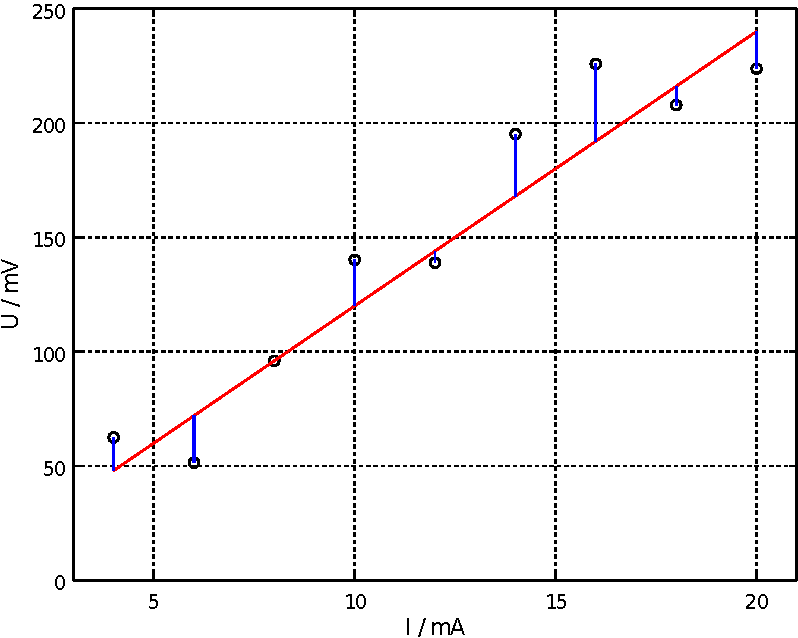
\includegraphics[width=80mm]{01_vorlesung/media/learn_estimation_ohm.pdf}
\caption{Regressionbeispiel: Modellparameter finden, dessen Wert am besten zu den Daten passt}
\label{Ohm1}
\end{center}
\end{figure}

Ob die Spannungswerte zu dem Modell \glqq passen\grqq ~wird bewertet, wobei das Modell
besagt, dass die Spannungswerte gleich dem Widerstand, der genau eine konstante Größe sein soll,
multipliziert mit den eingestellten Werten der Stromstärke seien. Das Bewertungskriterium ist
\glqq die Treffer-Wahrscheinlichkeit Spannungswert liegt auf Widerstand mal Strom\grqq.
Wir gehen davon aus, dass die Abweichungen $\varepsilon_i \; = \; U_i \, - \, R I_i$ normalverteilt sind, also
\begin{equation}
p(U_i,I_i | R) \; \propto \; e^{-\frac{1}{2} \left(\frac{\varepsilon_i}{\sigma_\varepsilon}\right)^2}
\end{equation}
wobei $\sigma_\varepsilon$ ein Maß für die Streuung der Residuen, hier in Millivolt, ist.
Wir haben die Werte der Abweichungen $\varepsilon_i$. Man nennt sie \textbf{Residuen}.
Das Produkt aller Wahrscheinlichkeiten $p(U_i,I_i | R)$ heißt \textbf{Likelihood}.
\begin{equation}
L((U_1,\dots, U_J), (I_1,\dots,I_J) | R) \; = \; \prod\limits_{i = 1}^J \, p(U_i,I_i | R)
\end{equation}
Unsere Modellparameter bzw.\ der Modellparameter, die bzw.\ den wir ermitteln wollen, ist $R$ und
für die Streuung der Werte des Parameters $R$ verwenden wir das Formelzeichen $\sigma_R$.

In der frequentistischen Statistik wird von der Vorstellung ausgegangen, dass es einen wahren Wert für
$R$ gibt, dem man sich nähert, je mehr und genauer man misst, der aber wegen der Streuung
der Spannungswerte $U$ nur annähernd bestimmbar ist. Wenn wir die Präzisionsstromquelle unverändert
auf einen festen Wert einstellen und nicht durchfahren und dann mehrfach die Spannungen ablesen, so
beobachten wir dennoch leicht unterschiedliche Werte für die Spannung. Dies ist der Grund dafür
dass die Wertepaare bei durchgefahrenem Strom $(I_j, U_j)$ nicht exakt auf einer Geraden liegen.

Am besten passt das ganze für einen Wert für $R$,
für den $L((U_1,\dots, U_J), (I_1,\dots,I_J) | R)$ maximal wird.
Die Zielfunktion unseres Optimierungsvorgangs ist also:
\begin{equation}
\max_{R} \; L((U_1,\dots, U_J), (I_1,\dots,I_J) | R)
\end{equation}
Solch eine Optimierungsaufgabe heißt \textbf{Maximum-Likelihood}-Verfahren.
\begin{equation}
\max_{R} \; \prod\limits_{i = 1}^J \,  e^{-\frac{1}{2} \left(\frac{\varepsilon_i}{\sigma_\varepsilon}\right)^2}
\label{MaxiLikeR1}
\end{equation}
d.h.\ nach den Gesetzen der Potenzrechnung
\begin{equation}
\max_{R} \; e^{-\frac{1}{2} \sum\limits_{i = 1}^J \, \left(\frac{\varepsilon_i}{\sigma_\varepsilon}\right)^2} .
\label{MaxiLikeR2}
\end{equation}
Das Maximum der Gaußfunktion liegt an der Stelle, an der der Exponent minimal wird.
Wir maximieren die Likelihood, wenn wir ihren Logarithmus minimieren:
\begin{equation}
\min_{R} \; \sum_{i = 1}^J \, \left(\frac{\varepsilon_i}{\sigma_\varepsilon}\right)^2
\label{MaxiLikeLSQ}
\end{equation}
dazu suchen wir die Nullstelle der Ableitung nach dem Modellparameter.
Auf die Suche des Minimums wird auch mit dem Terminus \textsl{Methode der kleinsten Abweichungsquadrate} oder
\textsl{Least Mean Square Method} Bezug genommen.
Hätten wir nicht nur $R$ sondern viele,
dann würden wir den Gradienten bilden.
\begin{equation}
\frac{\partial}{\partial R} \; \sum_{i = 1}^J \, \left(\frac{\varepsilon_i}{\sigma_\varepsilon}\right)^2 \; = \; 0
\end{equation}
d.i.\ in unserem Beispiel
\begin{equation}
\frac{\partial}{\partial R} \; \sum_{i = 1}^J \, \left(\frac{U_i \, - \, R \, I_i}{\sigma_\varepsilon}\right)^2 \; = \; 0
\end{equation}
Wir multiplizieren mit dem Faktor $\sigma_\varepsilon$
\begin{equation}
\frac{\partial}{\partial R} \; \sum_{i = 1}^J \, \left(U_i \, - \, R \, I_i\right)^2 \; = \; 0
\end{equation}
und führen die Differentiation durch
\begin{equation}
\sum_{i = 1}^J \, 2 \left(U_i \, - \, R \, I_i\right) \, I_i \; = \; 0 .
\end{equation}
Für viele Modellparameter gäbe es entsprechend viele solche Gleichungen mit den jeweiligen Ableitungen, so dass
dann hier ein lineares Gleichungssystem stünde, das zu lösen wäre.
Ein numerisches Verfahren zur Lösung linearer Gleichungssysteme ist das Gauß-Jordan-Eliminationsverfahren.
Nun wir nur diese eine Gleichung haben, können wir einfach nach $R$ auflösen.
\begin{equation}
\sum_{i = 1}^J \, U_i \, I_i \; = \; \sum_{i = 1}^J \, R \, I_i \, I_i
\end{equation}
d.h.
\begin{equation}
 R \; = \; \frac{\sum\limits_{i = 1}^N \, U_i \, I_i}{\sum\limits_{i = 1}^N \,  I_i^2}
\end{equation}
Der ermittelte Wert für $R$ mit den Daten aus der Tabelle ist $12.34~\mathrm{\Omega}$, siehe Abb.~\ref{OhmResult}

\begin{figure}
\begin{center}
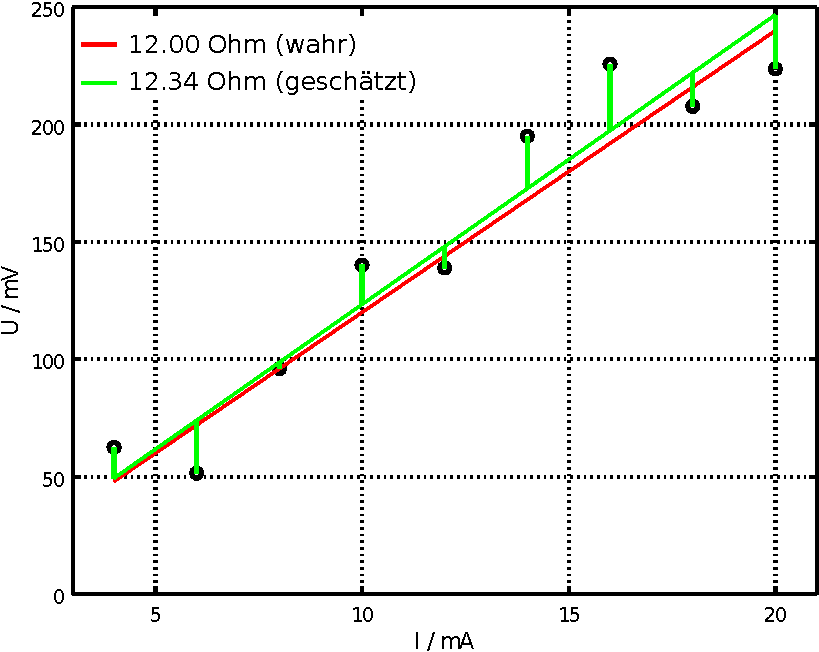
\includegraphics[width=80mm]{01_vorlesung/media/learn_estimation_ohm_esti.pdf}
\label{OhmResult}
\caption{Regressionsbeispiel: Der geschätze Wert des Modellparameters im Vergleich zum wahren.}
\end{center}
\end{figure}

Zuvor haben wir die Likelihood ohne Normierungsfaktor aufgeschrieben.
Eine Wahrscheinlichkeitsdichteverteilung ist so definiert, dass die Fläche unter ihrer Kurve 1 ist, also die Wahrscheinlichkeit
für das Beobachten jedes beliebigen Wertes immer voll eintritt.
\begin{equation}
p(\varepsilon) \; = \; \frac{1}{\sqrt{2 \pi} \sigma_{\varepsilon}} \, e^{-\frac{1}{2} \left(\frac{\varepsilon}{\sigma_{\varepsilon}}\right)^2}
\end{equation}
Ein Maß für die Breite der Gaußglocke ist das $\sigma_{\varepsilon}$ bei etwa 60 Prozent der Höhe ($e^{-\frac{1}{2}} \approx 0.6$).
Ihr Quadrat wird \textbf{Varianz} genannt.
\begin{figure}
\begin{center}
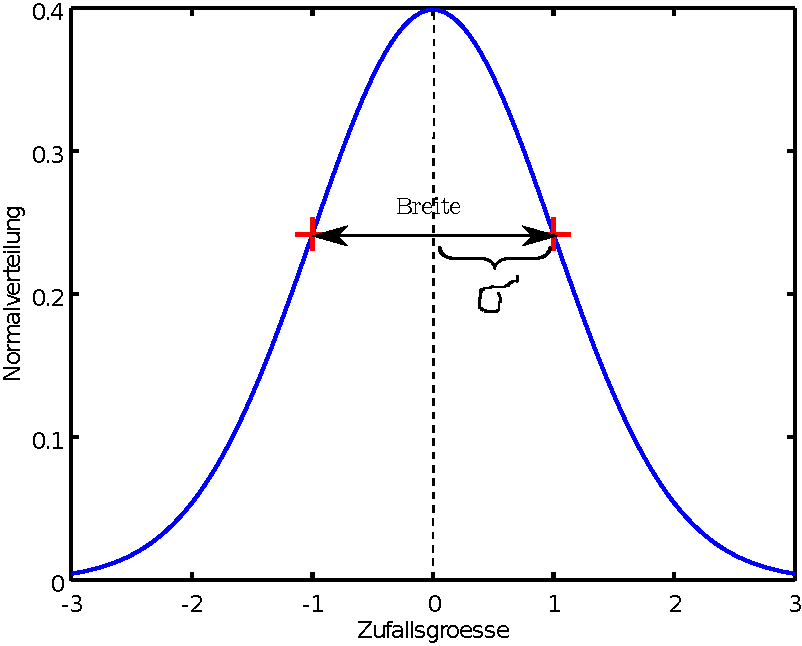
\includegraphics[width=80mm]{01_vorlesung/media/breite_norm_pdf.pdf}
\label{normpdf}
\caption{Breite der Normalverteilung.}
\end{center}
\end{figure}
Das zweite statistische Moment dieser Verteilung 
\begin{equation}
\int_{-\infty}^\infty \, \varepsilon^2 \, p(\varepsilon) \, \mathrm{d} \varepsilon 
\end{equation}
ist gleich dem Quadrat von $\sigma_\varepsilon$, also der Varianz der Gaußverteilung
\begin{equation}
\int_{-\infty}^\infty \, \varepsilon^2 \,  \frac{1}{\sqrt{2 \pi} \sigma_{\varepsilon}} \, e^{-\frac{1}{2} \left(\frac{\varepsilon}{\sigma_\varepsilon}\right)^2} \, \mathrm{d} \varepsilon  \; = \; \sigma_{\varepsilon}^2 .
\end{equation}
Diskretisiert entspricht dies
\begin{equation}
\frac{1}{\sqrt{2 \pi} \sigma_\varepsilon} \, e^{-\frac{1}{2} \left(\frac{\varepsilon}{\sigma_{\varepsilon}}\right)^2} \, \mathrm{d} \varepsilon
\end{equation}
einer relativen Häufigkeit $\frac{n_k}{J-1}$ in der $k$-ten Klasse der Breite $\mathrm{d} \varepsilon$.
Wenn wir nun kein Histogramm mit gleichgroßen Klassenbreiten bilden, sondern zu jedem $\varepsilon_i$ eine Klasse mit der relativen
Häufigkeit $\frac{1}{J-1}$ betrachten, dann haben wir so ungefähr für das $\sigma_{\varepsilon}^2$
\begin{equation}
\sum_{i=1}^J \, \varepsilon_i^2 \,  \frac{1}{J-1}  \; \approx \; \sigma_{\varepsilon}^2 .
\end{equation}
Wir nennen diese Breite wegen der Näherung nicht $\sigma_{\varepsilon}^2$. Diese Näherung ist nur ein ungefährer Schätzwert 
und wird \textbf{empirische Varianz} genannt:
\begin{equation}
s_{\varepsilon}^2 \; = \; \frac{1}{J-1} \, \sum_{i=1}^J \, \varepsilon_i^2
\end{equation}
Wir unterscheiden zwischen der Varianz und der empirischen Varianz durch die Verwendung der
unterschiedlichen Formelzeichen $\sigma$ und $s$.

Uns interessiert aber nicht so sehr die Varianz der Residuen $\varepsilon$, die direkt der Varianz
der Spannungsmessung entspricht,
als viel mehr die Varianz des Modellparameters $R$.
Betrachte die Modellgleichung $R \; = \; \frac{U}{I}$, wie empfindlich reagiert die Größe $R$ auf Veränderung der Größe $U$.
Wählt man anstelle eines Wertes $U$ einen Wert $U \, + \, \Delta U$, so reagiert die Größe $R$ über die Modellgleichung wie folgt
\begin{equation}
R \, + \, \Delta R \; = \; \frac{1}{I} \, \left( U \, + \, \Delta U \right)
\end{equation}
d.i. mit $R \; = \; \frac{U}{I}$
\begin{equation}
\Delta R \; = \; \frac{1}{I} \, \left( \Delta U \right)
\end{equation}
Der Differenzenquotient ist also
\begin{equation}
\frac{\Delta R}{\Delta U} \; = \; \frac{1}{I}
\end{equation}
was bei diesem linearen Zusammenhang direkt hinkommt. Allgemein passt es für stetige Modelle auch bei nichtlinearem Zusammenhang
für genügend kleine Änderungen. Deshalb wird die Empfindlichkeit, die \textbf{Sensitivität}, definiert als die lokale Steigung
\begin{equation}
c  \; = \; \frac{\partial R}{\partial U}
\end{equation}
Die Varianz ist eine quadratische Veränderung, so dass
\begin{equation}
s_R^2  \; = \; \left(\frac{\partial R}{\partial U}\right)^2 \, s_{\varepsilon}^2 \; = \; \frac{1}{I^2} \, s_{\varepsilon}^2
\end{equation}
Hier hätte ich auch direkt $s_R$ aufschreiben können, aber die quadratische Schreibweise wird erforderlich, wenn es um mehrere Größen geht. In den folgenden Vorlesungen werden wir das Konzept der Fortpflanzung der Varianzen kennen lernen.

Die Varianzen sind ein Maß für die Unsicherheit von Messungen. Die \textbf{Messunsicherheit} ist zentrales Thema in der Messtechnik.
Im Wörterbuch der Metrologie (VIM)
\begin{verbatim}
https://www.bipm.org/utils/common/documents/jcgm/JCGM_200_2012.pdf
\end{verbatim}
wird sie wie folgt definiert:
\begin{quote}
\textbf{Messunsicherheit; Unsicherheit} (engl. \textsl{measurement uncertainty; uncertainty}): 
nichtnegativer Parameter, der die Streuung der Werte kennzeichnet, die der Messgröße
auf der Grundlage der benutzten Information beigeordnet ist. [VIM2.26]
\end{quote}
Sie drückt den Mangel einer genauen Kenntnis des Wertes der Messgröße aus.
Selbst wenn systematische Effekte korrigiert werden, bleibt der \textbf{Messwert} lediglich
ein \textbf{Schätz\-wert der Messgröße}, siehe auch GUM:2008, Abschnitt 3.3.1 .

Im Bereich der Metrologie wird zum Thema Messunsicherheitsberechnung eine Richtlinie verwendet,
um die Auswerteverfahren im gesetzlichen Messwesen zu vereinheitlichen und die Resultate
besser vergleichbar zu machen. Die Richtlinie wurde von der
\textsl{Working Group} 1 des \textsl{Joint Committee for Guides in Metrology} (JCGM/WG 1)
entwickelt. Sie hat den Titel \textsl{Evaluation of measurement
data - Guide to the expression of uncertainty in measurement} und wird mit GUM abgekürzt.
Die derzeit gültige Version ist
\textsl{JCGM 100:2008 GUM 1995 with minor corrections} und ist in englischer Fassung
auf der Webseite des \textsl{Bureau international des poids et mesures} (BIPM)
unter folgendem Link frei erhältlich:
\begin{verbatim}
https://www.bipm.org/utils/common/documents/jcgm/JCGM_100_2008_E.pdf
\end{verbatim}

In vielen Fällen reicht es, die Varianzen der einzelnen direkten Messgrößen zu untersuchen sowie
den Zusammenhang zwischen der Variation einer direkten Messgröße und die dadurch verusachte
Veränderung der indirekten, also die Empfindlichkeit/Sensitivität.
Dieser Zusammenhang ist zentrales Thema der Bestimmung von Messunsicherheiten
und wird im Laufe dieser Vorlesung eingehend beleuchtet.
Vielfach gibt es nicht nur einen Zusammenhang zwischen einer direkten mit einer indirekten Messgröße,
sondern auch einen Zusammenhang zwischen den direkten Messgrößen untereinander.

In dieser Vorlesungsreihe liegt das Hauptaugenmerk auf linearen Zusammenhängen zwischen Messgrößen.
Für viele Anwendungen greifen lineare Ansätze. Wenn die betrachteten Bereiche der Variation von Größen
genügend klein sind, so lassen sich auch nichtlineare Modelle durch eine Linearisierung in einer gewissen
Umgebung approximieren.

Das Maß für den linearen Zusammenhang wird \textbf{Korrelation} genannt.
Bei der linearen Regression geht es um Modelle mit indirekten Messgrößen,
die als Koeffizienten eines Polynoms auftreten. Um den Grad des Polynoms zu ermitteln, wird untersucht
mit welchem Potenzgesetz ein Paar direkter Messgrößen zu verknüpfen ist (welchen Grad das Polynom hat),
so dass die Korrelation groß ist.


\section{Charakterisierung von linearem Zusammenhang zwischen Größen}


Bei dem Beispiel mit dem Ohm'schen Gesetz hatten wir uns mit der Modellgleichung $U = R I$ befasst.
Dabei waren $U$ und $I$ die beiden physikalischen Größen, die unterschiedliche Werte angenommen haben und
über einen linearen Zusammenhang verknüpft sind. Hier haben wir also eine Gerade, Polynom vom Grad 1.

Für die Charakterisierung \textsl{linearer} Zusammenhänge ist der
\textbf{Korrelationskoeffizient} $\rho$ ein Maß, mit dem quantifiziert wird, wie
stark zwei Größen linear miteinander verknüpft sind.
Der Korrelationskoeffizient ist so definiert, dass er Werte zwischen $-1$ und
$1$ annehmen kann. Gibt es einen direkten linearen Zusammenhang zwischen zwei Zufallsgrößen
$X_1$ und $X_2$, so wird man zu einer Beobachtung der einen Größe mit kleinem Wert
auch einen kleinen Wert bei der anderen Größe beobachten und wenn die eine Größe einen
großen Wert annimmt, so wird die andere auch einen großen Wert annehmen, und
$\rho$ wird in der Nähe von $1$ liegen. Haben zwei Zufallsgrößen einen ebenso
direkten Zusammenhang, aber in umgekehrter Weise, dass zu kleinen Werten von der ersten
Größe große Werte zur zweiten Größe auftreten und umgekehrt, so liegt $\rho$ in der Nähe von $-1$.
In beiden Fällen sagt man, dass die Größen \textbf{korreliert} seien.

Gibt es überhaupt gar keinen Zusammenhang zwischen dem, was an Werten zu der einen Größe beobachtet
wird mit dem, so ist $\rho = 0$ und man sagt: Die beiden Größen seien \textbf{unkorreliert}.

\begin{figure}
	\begin{center}
		\includegraphics[width=75mm]{01_vorlesung/media/korreliert.pdf} \hspace{5mm}
		\includegraphics[width=75mm]{01_vorlesung/media/unkorreliert.pdf}
		\caption{\label{korrelation} Wenn es einen linearen Zusammenhang zwischen
			zwei Zufallsgrößen $X_1$ und $X_2$ gibt, so sagt man, dass sie korreliert sind
			und der Korrelationskoeffizient $\rho$ liegt bei Eins (\textsl{links}) oder bei
			minus Eins. Wenn es keinen Zusammenhang zwischen zwei Zufallsgrößen $X_1$ und $X_2$
			gibt, so sagt man, dass sie unkorreliert sind
			und der Korrelationskoeffizient $\rho$ liegt bei Null (\textsl{rechts}).}
	\end{center}
\end{figure}

Die Erwartungswerte zu jeder der Größen $X_1$ und $X_2$ sind jeweils
$\mathrm{E}(X_1)$ und $\mathrm{E}(X_2)$. Sie werden aus den Mittelwerten der jeweiligen
Stichproben geschätzt
\begin{equation}
\bar x_1 \; = \; \frac{1}{J} \, \sum_{j = 1}^J X_{1,j} \qquad
\bar x_2 \; = \; \frac{1}{J} \, \sum_{j = 1}^J X_{2,j}
\end{equation}
Dann ist
\begin{equation}
\mathrm{\bar X} \; = \;
\left(\begin{array}{c}
\bar x_1 \\
\bar x_2
\end{array}
\right)
\end{equation}
der Schwerpunkt der Beobachtungen der Größen.
Sind die Entfernungen der Beobachtungs\-pärchen $(X_{1,j}, X_{2,j})$ vom Schwerpunkt so,
dass die Richtungskomponente der Größe $X_1$ in die gleiche Richtung weist und auch in
proportionale Entfernung wie die Richtungskomponente der Größe $X_2$, so liefern die 
Produkte $(X_{1,j} - \bar x_1)(X_{2,j} - \bar x_2)$ gleiche Vorzeichen. Streuen diese
aber unzusammenhängend, so mitteln sich die unterschiedlichen Terme
$(X_{1,j} - \bar x_1)(X_{2,j} - \bar x_2)$ bei Summation weg.

Wir definieren die Größe
\begin{equation}
s_{1,2} \; := \; \frac{1}{J-1} \, \sum_{j = 1}^J (X_{1,j} - \bar x_1)(X_{2,j} - \bar x_2)
\end{equation}
und nennen sie die \textbf{empirische Kovarianz}.
Allgemein ist die \textbf{Kovarianz} für Zufallsgrößen, deren gemeinsame Verteilung
ihre Wahrscheinlichkeitsdichte $p(X_1, X_2)$ sei, wie folgt definiert
\begin{equation}
\operatorname{Cov}(X_1, X_2) \; := \; 
\int\limits_{-\infty}^{\infty}\int\limits_{-\infty}^{\infty}
(X_1^\prime \, - \operatorname{E}(X_1))(X_2^\prime \, - \operatorname{E}(X_2)) \,
p(X_1^\prime, X_2^\prime) \, \operatorname{d} X_1^\prime \operatorname{d} X_2^\prime .
\end{equation}
Wir sehen hier, dass die Kovarianz einer Zufallsgröße mit sich selbst die
\textbf{Varianz} ist
\begin{equation}
\operatorname{Var}(X_1) \; := \;  \operatorname{Cov}(X_1, X_1) \; = \; 
\int\limits_{-\infty}^{\infty}
(X_1^\prime \, - \operatorname{E}(X_1))^2 \,
p(X_1^\prime) \, \operatorname{d} X_1^\prime
\end{equation}
und für die empirsche Varianz und Kovarianz gilt entsprechend
\begin{equation}
s_{1}^2 \; := \; s_{1,1} \; = \; 
\frac{1}{J-1} \, \sum_{j = 1}^J (X_{1,j} - \bar x_1)^2 .
\end{equation}
Wir werden im nächsten Kapitel sehen, dass bei der Steigung der Regressionsgraden
(Aufgabe 1) genau so ein Term $\sum_{j = 1}^J (X_{1,j} - \bar x_1)(X_{2,j} - \bar x_2)$
im Zähler steht.

Für das Verständnis der Gesamtzusammenhänge ist der Sprachgebrauch für Zufallsgrößen sowie
der Sprachgebrauch des Erwartungswertes von Zufallgrößen von Bedeutung. 

Verknüpfungen von Zufallsgrößen sind ihrerseits wieder Zufallsgrößen. Betrachten
wir eine Größe $X$, die ganz abstrakt und allgemein eine Zufallsgröße ist, und
$p(X)$ die Wahrscheinlichkeitsdichteverteilung dazu, so heißt
\begin{equation}
\operatorname{E}(X) \; := \;  \int\limits_{-\infty}^{\infty}
X^\prime \, p(X^\prime) \, \operatorname{d} X^\prime
\end{equation}
Erwartungswert der Zufallsgröße $X$.
Ist diese Zufallsgröße eine Verknüpfung von anderen Zufallsgrößen und setzen wir die
Verknüpfung ein, so wird der Erwartungwert mit derselben Verknüpfung gebildet.
Betrachten wir zum Beispiel die Verknüpfung Addition $X = X_1 + X_2$
\begin{equation}
\operatorname{E}(X_1 + X_2) \; := \;  \int\limits_{-\infty}^{\infty} \int\limits_{-\infty}^{\infty}
(X_1^\prime + X_2^\prime) \, p(X_1^\prime, X_2^\prime) \, \operatorname{d} X_1^\prime \, \operatorname{d} X_2^\prime
\end{equation}
d.h.
\begin{equation}
\arraycolsep=2.0pt\def\arraystretch{2.0}
\begin{array}{ll}
\operatorname{E}(X_1 + X_2) \; = & \int\limits_{-\infty}^{\infty} \int\limits_{-\infty}^{\infty}
X_1^\prime \, p(X_1^\prime, X_2^\prime) \, 
\operatorname{d} X_1^\prime \, \operatorname{d} X_2^\prime\\
& + \; \int\limits_{-\infty}^{\infty} \int\limits_{-\infty}^{\infty} 
X_2^\prime \, p(X_1^\prime, X_2^\prime) \, \operatorname{d} X_1^\prime \, \operatorname{d} X_2^\prime
\end{array}
\end{equation}
und mit der Randverteilung (engl.\ \textsl{marginal distribution}) 
\begin{equation}
p(X_2) \; = \;
\int\limits_{-\infty}^{\infty} p(X_1^\prime, X_2) \, \operatorname{d} X_1^\prime
\label{marginalDistr}
\end{equation}
erhalten wir
\begin{equation}
\operatorname{E}(X_1 + X_2) \; = \; \int\limits_{-\infty}^{\infty}
X_1^\prime \, p(X_1^\prime) \, \operatorname{d} X_1^\prime 
\; + \; \int\limits_{-\infty}^{\infty} 
X_2^\prime \, p(X_2^\prime) \, \operatorname{d} X_2^\prime
\end{equation}
also
\begin{equation}
\operatorname{E}(X_1 + X_2) \; = \; \operatorname{E}(X_1) \; + \; \operatorname{E}(X_2).
\label{EwSummeISTSummeEw}
\end{equation}
In Worten heißt dies: Der Erwartungswert einer Summe von Zufallsgrößen ist die
Summe der Erwartungswerte der Zufallsgrößen.

Als nächstes betrachten wir das Produkt zweier Zufallsgrößen
$X = X_1 \cdot X_2$
\begin{equation}
\operatorname{E}(X_1 \cdot X_2) \; := \; 
\int\limits_{-\infty}^{\infty} \int\limits_{-\infty}^{\infty}
X_1^\prime \, X_2^\prime \; p(X_1^\prime, X_2^\prime) \,
\operatorname{d} X_2^\prime\, \operatorname{d} X_1^\prime .
\end{equation}
Die Kovarianz ist der Erwartungswert folgenden Produktes
$(X_1 - \operatorname{E}(X_1)) \cdot (X_2 - \operatorname{E}(X_2))$
\begin{equation}
\operatorname{E}((X_1 - \operatorname{E}(X_1)) \cdot
(X_2 - \operatorname{E}(X_2))) \; = \; 
\int\limits_{-\infty}^{\infty} \int\limits_{-\infty}^{\infty}
(X_1^\prime - \operatorname{E}(X_1)) \cdot (X_2^\prime - \operatorname{E}(X_2))
\, p(X_1^\prime, X_2^\prime) \, 
\operatorname{d} X_1^\prime\, \operatorname{d} X_2^\prime
\end{equation}
also
\begin{equation}
\operatorname{Cov}(X_1, X_2)  \; = \; \operatorname{E}\left((X_1 - \operatorname{E}(X_1)) 
\cdot (X_2 - E(X_2)) \right)  .
\end{equation}
Ferner ist zu bemerken, dass sich aus diesen Beziehungen für die
Kovarianz ergibt
\begin{equation}
\begin{array}{ll}
\operatorname{Cov}(X_1, X_2)
& \; = \;  \operatorname{E}\left(X_1 \, X_2 - X_2 \, \operatorname{E}(X_1) -
X_1 \, \operatorname{E}(X_2) + \operatorname{E}(X_1) \, \operatorname{E}(X_2) \right) \\
& \; = \;  \operatorname{E}(X_1 \, X_2)  - \operatorname{E}(X_2) \, \operatorname{E}(X_1)
- \operatorname{E}(X_1) \, \operatorname{E}(X_2) + \operatorname{E}(X_1) \, \operatorname{E}(X_2)) \\
& \; = \;  \operatorname{E}(X_1 \, X_2) - \operatorname{E}(X_1) \, \operatorname{E}(X_2) .
\end{array}
\label{ErwartungsCOV}
\end{equation}
Per Definitionem gilt
\begin{equation}
\operatorname {Var}(X) \; := \; \operatorname {Cov}(X,X) .
\end{equation}
Daraus folgt, dass für die Varianz einer Zufallsgröße,
die das Produkt einer Zufallsgröße $X$ mit einem konstanten, festen reellen Faktor $b$ ist, gilt
\begin{equation}
\operatorname {Var}(b X) \; := \; b^2 \, \operatorname {Var}(X)
\end{equation}
%Für einen Zufallsgrößenvektor $\boldsymbol{X}$ multipliziert mit einer Matrix 
%$\boldsymbol{B}$, deren Elemente konstante, feste reelle Zahlen sind, gilt entsprechend
%\begin{equation}
%\operatorname {Cov}(\boldsymbol{B} \boldsymbol{X}) \; := \; \boldsymbol{B} \,
% \operatorname {Cov}(\boldsymbol{X}) \, \boldsymbol{B}^\mathsf{T} .
%\label{CovarianzKonstMatrix}
%\end{equation}
%Das ist jetzt nicht trivial herzuleiten, aber wir wollen jetzt keine Vorlesung in Lineare
%Algebra halten. Wir werden diese Beziehung für die Bestimmung der Standardabweichung der
%Modellparameter in der linearen Regression brauchen. Das hochgestellte $\mathsf{T}$ steht für
%transponiert.

Eine weitere wichtige Beziehung ist folgende zur
\textbf{Varianz einer Summe von Zufallsgrößen}:
\begin{equation}
\operatorname {Var}\left(\sum _{{i=1}}^{N}X_{i}\right) \; = \;
\sum _{{i,j=1}}^{N}\operatorname {Cov}(X_{i},X_{j})
\label{VarianzSummeISTSummeKovarianz}
\end{equation}
Die Varianz ist nach Definition
\begin{equation}
\operatorname {Var}\left(\sum _{{i=1}}^{N}X_{i}\right) \; = \;
\int\limits_{-\infty}^{\infty} \dots \int\limits_{-\infty}^{\infty}
\, \left[ \left(\sum_{i=1}^N X_i\right) \; - \; E(\sum_{i=1}^N X_i) \right]^2 \, p(X_1, \dots, X_2)
\, \operatorname{d}X_1 \dots \operatorname{d}X_N .
\end{equation}
Da der Erwartungswert einer Summe von Zufallsgrößen gleich der Summe der 
Erwartungswerte jeder einzelnen dieser Zufallsgrößen ist, siehe Gl.~(\ref{EwSummeISTSummeEw}), gilt
$$
\left(\sum_{i=1}^N X_i \right) \; - \; E(\sum_{i=1}^N X_i) \; = \;
\left(\sum_{i=1}^N X_i \right) \; - \; \sum_{i=1}^N E(X_i) 
$$
so dass gilt
\begin{equation}
\operatorname {Var}\left(\sum _{{i=1}}^{N}X_{i}\right) \; = \;
\int\limits_{-\infty}^{\infty} \dots \int\limits_{-\infty}^{\infty}
\, \left[ \sum_{i=1}^N \left(X_i \; - \; E(X_i)\right) \right]^2 \, p(X_1, \dots, X_2)
\, \operatorname{d}X_1 \dots \operatorname{d}X_N .
\end{equation}
Mit Anwendung des Assoziativgesetzes
$$
\arraycolsep=3.5pt\def\arraystretch{1.8}
\begin{array}{ll}
\left[ \sum\limits_{i=1}^N \left(X_i \; - \; E(X_i)\right) \right]^2 & =
\left[ \sum\limits_{i=1}^N \left(X_i \; - \; E(X_i)\right) \right] \;
\left[ \sum\limits_{k=1}^N \left(X_k \; - \; E(X_k)\right) \right] \\
& = \sum\limits_{i=1}^N \sum\limits_{k=1}^N  \left(X_i \; - \; E(X_i)\right) \;
\left(X_k \; - \; E(X_k)\right) \\
\end{array}
$$
gilt
\begin{equation}
\operatorname {Var}\left(\sum _{{i=1}}^{N}X_{i}\right) \; = \;
\int\limits_{-\infty}^{\infty} \dots \int\limits_{-\infty}^{\infty}
\, \sum_{i=1}^N \sum_{k=1}^N  \left(X_i \; - \; E(X_i)\right) \;
\left(X_k \; - \; E(X_k)\right) \, p(X_1, \dots, X_2)
\, \operatorname{d}X_1 \dots \operatorname{d}X_N .
\end{equation}
Durch Berechnung der Marginalverteilungen und weil $\int p(X_j) \, \operatorname{d}X_j = 1$
für alle $j$, die weder $i$ noch $k$ sind, erhalten wir
\begin{equation}
\operatorname {Var}\left(\sum _{{i=1}}^{N}X_{i}\right) \; = \;
\sum_{i=1}^N \sum_{k=1}^N  \;
\int\limits_{-\infty}^{\infty} \int\limits_{-\infty}^{\infty}
\, \left(X_i \; - \; E(X_i)\right) \;
\left(X_k \; - \; E(X_k)\right) \, p(X_i, X_k)
\, \operatorname{d}X_i \operatorname{d}X_k .
\end{equation}
Der Term auf der rechten Seite ist genau die Kovarianz der beiden 
Größen $X_i$ und $X_k$.

Die Beziehung Gl.~(\ref{VarianzSummeISTSummeKovarianz}), dass die
Varianz der Summe von Zufallsgrößen gleich der Summe der paarweisen Kovarianzen
ist, werden wir im Laufe dieser Vorlesungsreihe häufig
verwenden:
\begin{equation}
{\begin{aligned}\operatorname {Var}\left(\sum _{{i=1}}^{N}X_{i}\right) & 
	= \sum _{i=1}^{N}\sum _{k=1}^{N}\operatorname {Cov}(X_{i},X_{k})\\
	& = \sum _{{i=1}}^{N}\operatorname {Var}(X_{i})+
	\sum _{{i,k=1,i\neq k}}^{N}\operatorname {Cov}(X_{i},X_{k})\\
	& = \sum _{i=1}^{N}\operatorname {Var}(X_{i})+2\sum _{{i=1}}^{{N-1}}
	\sum _{k=i+1}^{N}\operatorname {Cov}(X_{i},X_{k}) ,
	\end{aligned}}
\label{VarianzSummeX2Kovarianz}
\end{equation}
Dies lässt sich für den Fall erweitern, dass die summierten Zufallsgrößen mit jeweils einem reellen,
konstanten Faktor multipliziert werden:
\begin{equation}
{\begin{aligned}\operatorname {Var}\left(\sum _{{i=1}}^{N} \, c_i \, X_{i}\right) & 
	= \sum _{i=1}^{N}\sum _{k=1}^{N}\operatorname {Cov}(c_i X_{i}, c_k X_{k})\\
	& = \sum _{{i=1}}^{N} \, c_i^2 \, \operatorname {Var}(X_{i})+
	\sum _{{i,k=1,i\neq k}}^{N} \, c_i c_k \,  \operatorname {Cov}(X_{i},X_{k})\\
	& = \sum _{{i=1}}^{N} \, c_i^2 \operatorname {Var}(X_{i})+2\sum _{{i=1}}^{{N-1}}
	\sum _{{k=i+1}}^{N} \, c_i c_k \operatorname {Cov}(X_{i},X_{k}).
	\end{aligned}}
\label{KovarianzSumme}
\end{equation}
Auf Gleichung (\ref{KovarianzSumme}) werden wir in den nächsten Vorlesungen zurück kommen,
denn diese ist die Grundlage für das \textbf{Gesetz zur Fortpflanzung von Messunsicherheiten}.

Für standardnormalverteilte Zufallsgrößen $Z_i$ mit $Z \sim \mathcal{N}(0,1)$ 
und $i = 1,2$ in die sich
die Größen $X_i$ wie folgt umrechnen lassen
\begin{equation}
Z_i \; = \; \frac{X_i \, - \, \operatorname{E}(X_i)}{\sqrt{\operatorname {Var}(X_{i})}}
\end{equation}
ist die Kovarianz gleich dem Korrelationskoeffizienten
\begin{equation}
\rho_{i,k} \; = \; \operatorname {Cov}(Z_{i},Z_{k})
\end{equation}
was äquivalent ist zu
\begin{equation}
\rho_{i,k} \; = \; \frac{\operatorname {Cov}(X_{i},X_{k})}{\sqrt{\operatorname {Var}(X_{i})} \, \sqrt{\operatorname {Var}(X_{k})}} .
\end{equation}


\section{Beispiel zum Selbststudium}
Zu Bestimmen ist ein Ohmscher Widerstand $R$ sowie eine Offsetspannung $U_0$ bei gegebenen Werten einer
Präzisionsstromquelle und eines Voltmeters:

\begin{center}
\begin{tabular}{l||c|c|c|c|c|c|c|c|c}
\hline\hline
 $I$ in mA &    4.0 &     6.0 &     8.0 &    10.0 &    12.0 &    14.0 &    16.0 &    18.0 &    20.0\\
\hline
 $U$ in mV &    62.5 &    51.5 &    96.0 &   140.2 &   138.9 &   195.1 &   225.8 &   207.8 &   223.7 \\
\hline\hline
\end{tabular}
\end{center}

Es wird angenommen, dass die Stromstärken ohne Streuung vorliegen (als Regressoren) und die Spannungen normalverteilt
streuen (als Regressanden), so dass
\begin{equation}
\min_{R, U_0} \; \sum_{i = 1}^J \, \left(U_i \, - \, R \, I_i  \, - \,  U_0\right)^2
\label{regrGer}
\end{equation}

\begin{itemize}
\item[(a)] Berechnen Sie den Korrelationskoeffizienten $\rho(I, U)$
\item[(b)] Lösen Sie das Gleichungssystem
\begin{equation}
\left(\begin{array}{c}
\frac{\partial}{\partial R}\\
\frac{\partial}{\partial U_0}
\end{array}\right)
\, \sum_{i = 1}^J \, \left(U_i \, - \, R \, I_i  \, - \,  U_0\right)^2 \; = \;
\left(\begin{array}{c}
0\\
0
\end{array}\right)
\label{regrGerGS}
\end{equation}
\item[(c)] Berechnen Sie die aus der Lösung des Gleichungssystems aus (a) gewonnen Schätzwerte
für $R$ und $U_0$.
\end{itemize}




%
\chapter{Konzepte der Statistik für die Messdatenanalyse}
\section{Charakterisierung von Beziehungen zwischen Größen}

Für eine Bewertung von Wechselwirkungen zwischen Effekten werden in der Statistik Maße
definiert, die die Stärke und eventuell auch Richtung eines Zusammenhangs zwischen dem
Auftreten zufälliger Ereignisse quantifizieren sollen. Wir hatten das Beispiel des Ohm'schen
Gesetzes betrachtet, bei dem es einen Zusammenhang zwischen Stromstärke und elektrischer
Spannung gibt. Der Zusammenhang ist in diesem Beispiel ein linearer.

Für die Charakterisierung \textsl{linearer} Zusammenhänge ist der
\textbf{Korrelationskoeffizient} $\rho$ ein Maß, mit dem quantifiziert wird, wie
stark zwei Größen linear miteinander verknüpft sind.
Der Korrelationskoeffizient ist definiert, dass er Werte zwischen $-1$ und
$1$ annehmen kann. Gibt es einen direkten linearen Zusammenhang zwischen zwei Zufallsgrößen
$X_1$ und $X_2$, so wird man zu einer Beobachtung der einen Größe mit kleinem Wert
auch einen kleinen Wert bei der anderen Größe beobachten und wenn die eine Größe einen
großen Wert annimmt, so wird die andere auch einen großen Wert annehmen, und
$\rho$ wird in der Nähe von $1$ liegen. Haben zwei Zufallsgrößen einen ebenso
direkten Zusammenhang, aber in umgekehrter Weise, dass zu kleinen Werten von der ersten
Größe große Werte zur zweiten Größe auftreten und umgekehrt, so liegt $\rho$ in der Nähe von $-1$.
In beiden Fällen sagt man, dass die Größen \textbf{korreliert} seien.

Gibt es überhaupt gar keinen Zusammenhang zwischen dem, was an Werten zu der einen Größe beobachtet
wird mit dem, was an Werten zu der anderen Größe beobachtet wird, so ist $\rho = 0$ und man
sagt die beiden Größen seien \textbf{unkorreliert}.

\begin{figure}
	\begin{center}
		\includegraphics[width=75mm]{02_vorlesung/media/korreliert.pdf} \hspace{5mm}
		\includegraphics[width=75mm]{02_vorlesung/media/unkorreliert.pdf}
		\caption{\label{korrelation} Wenn es einen linearen Zusammenhang zwischen
			zwei Zufallsgrößen $X_1$ und $X_2$ gibt, so sagt man, dass sie korreliert sind
			und der Korrelationskoeffizient $\rho$ liegt bei Eins (\textsl{links}) oder bei
			minus Eins. Wenn es keinen Zusammenhang zwischen zwei Zufallsgrößen $X_1$ und $X_2$
			gibt, so sagt man, dass sie unkorreliert sind
			und der Korrelationskoeffizient $\rho$ liegt bei Null (\textsl{rechts}).}
	\end{center}
\end{figure}

Die Erwartungswerte zu jeder der Größen $X_1$ und $X_2$ sind jeweils
$\mathrm{E}(X_1)$ und $\mathrm{E}(X_2)$. Sie werden aus den Mittelwerten der jeweiligen
Stichproben geschätzt
\begin{equation}
\bar x_1 \; = \; \frac{1}{J} \, \sum_{j = 1}^J X_{1,j} \qquad
\bar x_2 \; = \; \frac{1}{J} \, \sum_{j = 1}^J X_{2,j}
\end{equation}
Dann ist
\begin{equation}
\mathrm{\bar X} \; = \;
\left(\begin{array}{c}
\bar x_1 \\
\bar x_2
\end{array}
\right)
\end{equation}
der Schwerpunkt der Beobachtungen der Größen.
Sind die Entfernungen der Beobachtungs\-pärchen $(X_{1,j}, X_{2,j})$ vom Schwerpunkt so,
dass die Richtungskomponente der Größe $X_1$ in die gleiche Richtung weist und auch in
proportionale Entfernung wie die Richtungskomponente der Größe $X_2$, so liefern die 
Produkte $(X_{1,j} - \bar x_1)(X_{2,j} - \bar x_2)$ gleiche Vorzeichen. Streuen diese
aber unzusammenhängend, so mitteln sich die unterschiedlichen Terme
$(X_{1,j} - \bar x_1)(X_{2,j} - \bar x_2)$ bei Summation weg.

Wir definieren die Größe
\begin{equation}
s_{1,2} \; := \; \frac{1}{J-1} \, \sum_{j = 1}^J (X_{1,j} - \bar x_1)(X_{2,j} - \bar x_2)
\end{equation}
und nennen sie die \textbf{empirische Kovarianz}.
Allgemein ist die \textbf{Kovarianz} für Zufallsgrößen, deren gemeinsame Verteilung
ihre Wahrscheinlichkeitsdichte $p(X_1, X_2)$ sei, wie folgt definiert
\begin{equation}
\operatorname{Cov}(X_1, X_2) \; := \; 
\int\limits_{-\infty}^{\infty}\int\limits_{-\infty}^{\infty}
(X_1^\prime \, - \operatorname{E}(X_1))(X_2^\prime \, - \operatorname{E}(X_2)) \,
p(X_1^\prime, X_2^\prime) \, \operatorname{d} X_1^\prime \operatorname{d} X_2^\prime .
\end{equation}
Wir sehen hier, dass die Kovarianz einer Zufallsgröße mit sich selbst die
\textbf{Varianz} ist
\begin{equation}
\operatorname{Var}(X_1) \; := \;  \operatorname{Cov}(X_1, X_1) \; = \; 
\int\limits_{-\infty}^{\infty}
(X_1^\prime \, - \operatorname{E}(X_1))^2 \,
p(X_1^\prime) \, \operatorname{d} X_1^\prime
\end{equation}
und für die empirsche Varianz und Kovarianz gilt entsprechend
\begin{equation}
s_{1}^2 \; := \; s_{1,1} \; = \; 
\frac{1}{J-1} \, \sum_{j = 1}^J (X_{1,j} - \bar x_1)^2 .
\end{equation}
Wir haben bereits in der 2. Vorlesung gesehen, dass bei der Steigung der Regressionsgraden
(Aufgabe 1) genau so ein Term $\sum_{j = 1}^J (X_{1,j} - \bar x_1)(X_{2,j} - \bar x_2)$
im Zähler steht.

Für das Verständnis der Gesamtzusammenhänge ist der Sprachgebrauch für Zufallsgrößen sowie
der Sprachgebrauch des Erwartungswertes von Zufallgrößen von Bedeutung. 

Verknüpfungen von Zufallsgrößen sind ihrerseits wieder Zufallsgrößen. Betrachten
wir eine Größe $X$, die ganz abstrakt und allgemein eine Zufallsgröße ist, und
$p(X)$ die Wahrscheinlichkeitsdichteverteilung dazu, so heißt
\begin{equation}
\operatorname{E}(X) \; := \;  \int\limits_{-\infty}^{\infty}
X^\prime \, p(X^\prime) \, \operatorname{d} X^\prime
\end{equation}
Erwartungswert der Zufallsgröße $X$.
Ist diese Zufallsgröße eine Verknüpfung von anderen Zufallsgrößen und setzen wir die
Verknüpfung ein, so wird der Erwartungwert mit derselben Verknüpfung gebildet.
Betrachten wir zum Beispiel die Verknüpfung Addition $X = X_1 + X_2$
\begin{equation}
\operatorname{E}(X_1 + X_2) \; := \;  \int\limits_{-\infty}^{\infty} \int\limits_{-\infty}^{\infty}
(X_1^\prime + X_2^\prime) \, p(X_1^\prime, X_2^\prime) \, \operatorname{d} X_1^\prime \, \operatorname{d} X_2^\prime
\end{equation}
d.h.
\begin{equation}
\arraycolsep=2.0pt\def\arraystretch{2.0}
\begin{array}{ll}
\operatorname{E}(X_1 + X_2) \; = & \int\limits_{-\infty}^{\infty} \int\limits_{-\infty}^{\infty}
X_1^\prime \, p(X_1^\prime, X_2^\prime) \, 
\operatorname{d} X_1^\prime \, \operatorname{d} X_2^\prime\\
& + \; \int\limits_{-\infty}^{\infty} \int\limits_{-\infty}^{\infty} 
X_2^\prime \, p(X_1^\prime, X_2^\prime) \, \operatorname{d} X_1^\prime \, \operatorname{d} X_2^\prime
\end{array}
\end{equation}
und mit der Randverteilung (engl.\ \textsl{marginal distribution}) 
\begin{equation}
p(X_2) \; = \;
\int\limits_{-\infty}^{\infty} p(X_1^\prime, X_2) \, \operatorname{d} X_1^\prime
\label{marginalDistr}
\end{equation}
erhalten wir
\begin{equation}
\operatorname{E}(X_1 + X_2) \; = \; \int\limits_{-\infty}^{\infty}
X_1^\prime \, p(X_1^\prime) \, \operatorname{d} X_1^\prime 
\; + \; \int\limits_{-\infty}^{\infty} 
X_2^\prime \, p(X_2^\prime) \, \operatorname{d} X_2^\prime
\end{equation}
also
\begin{equation}
\operatorname{E}(X_1 + X_2) \; = \; \operatorname{E}(X_1) \; + \; \operatorname{E}(X_2).
\label{EwSummeISTSummeEw}
\end{equation}
In Worten heißt dies: Der Erwartungswert einer Summe von Zufallsgrößen ist die
Summe der Erwartungswerte der Zufallsgrößen.

Als nächstes betrachten wir das Produkt zweier Zufallsgrößen
$X = X_1 \cdot X_2$
\begin{equation}
\operatorname{E}(X_1 \cdot X_2) \; := \; 
\int\limits_{-\infty}^{\infty} \int\limits_{-\infty}^{\infty}
X_1^\prime \, X_2^\prime \; p(X_1^\prime, X_2^\prime) \,
\operatorname{d} X_2^\prime\, \operatorname{d} X_1^\prime .
\end{equation}
Die Kovarianz ist der Erwartungswert folgenden Produktes
$(X_1 - \operatorname{E}(X_1)) \cdot (X_2 - \operatorname{E}(X_2))$
\begin{equation}
\operatorname{E}((X_1 - \operatorname{E}(X_1)) \cdot
(X_2 - \operatorname{E}(X_2))) \; = \; 
\int\limits_{-\infty}^{\infty} \int\limits_{-\infty}^{\infty}
(X_1^\prime - \operatorname{E}(X_1)) \cdot (X_2^\prime - \operatorname{E}(X_2))
\, p(X_1^\prime, X_2^\prime) \, 
\operatorname{d} X_1^\prime\, \operatorname{d} X_2^\prime
\end{equation}
also
\begin{equation}
\operatorname{Cov}(X_1, X_2)  \; = \; \operatorname{E}\left((X_1 - \operatorname{E}(X_1)) 
\cdot (X_2 - E(X_2)) \right)  .
\end{equation}
Ferner ist zu bemerken, dass sich aus diesen Beziehungen für die
Kovarianz ergibt
\begin{equation}
\begin{array}{ll}
\operatorname{Cov}(X_1, X_2)
& \; = \;  \operatorname{E}\left(X_1 \, X_2 - X_2 \, \operatorname{E}(X_1) -
X_1 \, \operatorname{E}(X_2) + \operatorname{E}(X_1) \, \operatorname{E}(X_2) \right) \\
& \; = \;  \operatorname{E}(X_1 \, X_2)  - \operatorname{E}(X_2) \, \operatorname{E}(X_1)
- \operatorname{E}(X_1) \, \operatorname{E}(X_2) + \operatorname{E}(X_1) \, \operatorname{E}(X_2)) \\
& \; = \;  \operatorname{E}(X_1 \, X_2) - \operatorname{E}(X_1) \, \operatorname{E}(X_2) .
\end{array}
\label{ErwartungsCOV}
\end{equation}
Per Definitionem gilt
\begin{equation}
\operatorname {Var}(X) \; := \; \operatorname {Cov}(X,X) .
\end{equation}
Daraus folgt, dass für die Varianz einer Zufallsgröße,
die das Produkt einer Zufallsgröße $X$ mit einem konstanten, festen reellen Faktor $b$ ist, gilt
\begin{equation}
\operatorname {Var}(b X) \; := \; b^2 \, \operatorname {Var}(X)
\end{equation}
%Für einen Zufallsgrößenvektor $\boldsymbol{X}$ multipliziert mit einer Matrix 
%$\boldsymbol{B}$, deren Elemente konstante, feste reelle Zahlen sind, gilt entsprechend
%\begin{equation}
%\operatorname {Cov}(\boldsymbol{B} \boldsymbol{X}) \; := \; \boldsymbol{B} \,
% \operatorname {Cov}(\boldsymbol{X}) \, \boldsymbol{B}^\mathsf{T} .
%\label{CovarianzKonstMatrix}
%\end{equation}
%Das ist jetzt nicht trivial herzuleiten, aber wir wollen jetzt keine Vorlesung in Lineare
%Algebra halten. Wir werden diese Beziehung für die Bestimmung der Standardabweichung der
%Modellparameter in der linearen Regression brauchen. Das hochgestellte $\mathsf{T}$ steht für
%transponiert.

Eine weitere wichtige Beziehung ist folgende zur
\textbf{Varianz einer Summe von Zufallsgrößen}:
\begin{equation}
\operatorname {Var}\left(\sum _{{i=1}}^{N}X_{i}\right) \; = \;
\sum _{{i,j=1}}^{N}\operatorname {Cov}(X_{i},X_{j})
\label{VarianzSummeISTSummeKovarianz}
\end{equation}
Die Varianz ist nach Definition
\begin{equation}
\operatorname {Var}\left(\sum _{{i=1}}^{N}X_{i}\right) \; = \;
\int\limits_{-\infty}^{\infty} \dots \int\limits_{-\infty}^{\infty}
\, \left[ \left(\sum_{i=1}^N X_i\right) \; - \; E(\sum_{i=1}^N X_i) \right]^2 \, p(X_1, \dots, X_2)
\, \operatorname{d}X_1 \dots \operatorname{d}X_N .
\end{equation}
Da der Erwartungswert einer Summe von Zufallsgrößen gleich der Summe der 
Erwartungswerte jeder einzelnen dieser Zufallsgrößen ist, siehe Gl.~(\ref{EwSummeISTSummeEw}), gilt
$$
\left(\sum_{i=1}^N X_i \right) \; - \; E(\sum_{i=1}^N X_i) \; = \;
\left(\sum_{i=1}^N X_i \right) \; - \; \sum_{i=1}^N E(X_i) 
$$
so dass gilt
\begin{equation}
\operatorname {Var}\left(\sum _{{i=1}}^{N}X_{i}\right) \; = \;
\int\limits_{-\infty}^{\infty} \dots \int\limits_{-\infty}^{\infty}
\, \left[ \sum_{i=1}^N \left(X_i \; - \; E(X_i)\right) \right]^2 \, p(X_1, \dots, X_2)
\, \operatorname{d}X_1 \dots \operatorname{d}X_N .
\end{equation}
Mit Anwendung des Assoziativgesetzes
$$
\arraycolsep=3.5pt\def\arraystretch{1.8}
\begin{array}{ll}
\left[ \sum\limits_{i=1}^N \left(X_i \; - \; E(X_i)\right) \right]^2 & =
\left[ \sum\limits_{i=1}^N \left(X_i \; - \; E(X_i)\right) \right] \;
\left[ \sum\limits_{k=1}^N \left(X_k \; - \; E(X_k)\right) \right] \\
& = \sum\limits_{i=1}^N \sum\limits_{k=1}^N  \left(X_i \; - \; E(X_i)\right) \;
\left(X_k \; - \; E(X_k)\right) \\
\end{array}
$$
gilt
\begin{equation}
\operatorname {Var}\left(\sum _{{i=1}}^{N}X_{i}\right) \; = \;
\int\limits_{-\infty}^{\infty} \dots \int\limits_{-\infty}^{\infty}
\, \sum_{i=1}^N \sum_{k=1}^N  \left(X_i \; - \; E(X_i)\right) \;
\left(X_k \; - \; E(X_k)\right) \, p(X_1, \dots, X_2)
\, \operatorname{d}X_1 \dots \operatorname{d}X_N .
\end{equation}
Durch Berechnung der Marginalverteilungen und weil $\int p(X_j) \, \operatorname{d}X_j = 1$
für alle $j$, die weder $i$ noch $k$ sind, erhalten wir
\begin{equation}
\operatorname {Var}\left(\sum _{{i=1}}^{N}X_{i}\right) \; = \;
\sum_{i=1}^N \sum_{k=1}^N  \;
\int\limits_{-\infty}^{\infty} \int\limits_{-\infty}^{\infty}
\, \left(X_i \; - \; E(X_i)\right) \;
\left(X_k \; - \; E(X_k)\right) \, p(X_i, X_k)
\, \operatorname{d}X_i \operatorname{d}X_k .
\end{equation}
Der Term auf der rechten Seite ist genau die Kovarianz der beiden 
Größen $X_i$ und $X_k$.

Die Beziehung Gl.~(\ref{VarianzSummeISTSummeKovarianz}), dass die
Varianz der Summe von Zufallsgrößen gleich der Summe der paarweisen Kovarianzen
ist, werden wir im Laufe dieser Vorlesungsreihe häufig
verwenden:
\begin{equation}
{\begin{aligned}\operatorname {Var}\left(\sum _{{i=1}}^{N}X_{i}\right) & 
	= \sum _{i=1}^{N}\sum _{k=1}^{N}\operatorname {Cov}(X_{i},X_{k})\\
	& = \sum _{{i=1}}^{N}\operatorname {Var}(X_{i})+
	\sum _{{i,k=1,i\neq k}}^{N}\operatorname {Cov}(X_{i},X_{k})\\
	& = \sum _{i=1}^{N}\operatorname {Var}(X_{i})+2\sum _{{i=1}}^{{N-1}}
	\sum _{k=i+1}^{N}\operatorname {Cov}(X_{i},X_{k}) ,
	\end{aligned}}
\label{VarianzSummeX2Kovarianz}
\end{equation}
Dies lässt sich für den Fall erweitern, dass die summierten Zufallsgrößen mit jeweils einem reellen,
konstanten Faktor multipliziert werden:
\begin{equation}
{\begin{aligned}\operatorname {Var}\left(\sum _{{i=1}}^{N} \, c_i \, X_{i}\right) & 
	= \sum _{i=1}^{N}\sum _{k=1}^{N}\operatorname {Cov}(c_i X_{i}, c_k X_{k})\\
	& = \sum _{{i=1}}^{N} \, c_i^2 \, \operatorname {Var}(X_{i})+
	\sum _{{i,k=1,i\neq k}}^{N} \, c_i c_k \,  \operatorname {Cov}(X_{i},X_{k})\\
	& = \sum _{{i=1}}^{N} \, c_i^2 \operatorname {Var}(X_{i})+2\sum _{{i=1}}^{{N-1}}
	\sum _{{k=i+1}}^{N} \, c_i c_k \operatorname {Cov}(X_{i},X_{k}).
	\end{aligned}}
\label{KovarianzSumme}
\end{equation}
Auf Gleichung (\ref{KovarianzSumme}) werden wir in den nächsten Vorlesungen zurück kommen,
denn diese ist die Grundlage für das \textbf{Gesetz zur Fortpflanzung von Messunsicherheiten}.

Für standardnormalverteilte Zufallsgrößen $Z_i$ mit $Z \sim \mathcal{N}(0,1)$ 
und $i = 1,2$ in die sich
die Größen $X_i$ wie folgt umrechnen lassen
\begin{equation}
Z_i \; = \; \frac{X_i \, - \, \operatorname{E}(X_i)}{\sqrt{\operatorname {Var}(X_{i})}}
\end{equation}
ist die Kovarianz gleich dem Korrelationskoeffizienten
\begin{equation}
\rho_{i,k} \; = \; \operatorname {Cov}(Z_{i},Z_{k})
\end{equation}
was äquivalent ist zu
\begin{equation}
\rho_{i,k} \; = \; \frac{\operatorname {Cov}(X_{i},X_{k})}{\sqrt{\operatorname {Var}(X_{i})} \, \sqrt{\operatorname {Var}(X_{k})}} .
\end{equation}

Bei dem Beispiel mit dem Ohm'schen Gesetz hatten wir uns auch mit der Modellgleichung $U = R I$ befasst.
Dabei waren $U$ und $I$ die beiden physikalischen Größen, die unterschiedliche Werte angenommen haben und
einen starke Korrelation gezeigt haben, also einen linearen Zusammenhang. Ferner haben wir den Parameter
Widerstand $R$ geschätzt. Der Widerstand wurde also indirekt berechnet aus den direkt gemessenen Größen
$U$ und $I$. 

\newpage

\section{Konzept der Maximum-Likelihood-Methode zum Lösen inverser Probleme}

Bei der Messdatenanalyse geht es um die Schätzung von physikalischen Größen, die
indirekt über das Messen anderer Größen, direkter Messgrößen, ermittelt werden.
Die Aufgabe der Messtechnik lässt sich auch beschreiben als die Bestimmung
des Wertes von physikalischen Größen durch Messverfahren, die auf physikalischen Prinzipien
basieren. Die von einem Sensorsystem angezeigten Größen sind dabei
im allgemeinem andere Größen als diejenigen, die zu messen sind.

Wir hatten in der ersten Vorlesung zur Verdeutlichung der Aufgabenstellung
aus den einem Messsystem direkt zugänglichen Größen die gesuchten physikalischen
Größen zu gewinnen das Beispiel \glqq Beugung am Gitter\grqq ~betrachtet:
\begin{quote}
Ein Gitter wird mit kohärentem Licht beleuchtet. Das transmittierte Licht fällt auf eine CCD-Kamera, die
die Intensitäten in Abhängigkeit von der Position auf dem CCD-Chip aufnimmt. Es gibt dabei $N = 3$ direkte Größen:
zwei Ortskoordinaten $(x, y)$ auf dem CCD und der dazugehörige Intensitätswert $I$. Die Anzahl der CCD-Pixel ist die
Anzahl $J$ der Beobachtungen, $(x_1, y_1, I_1), \dots, (x_J, y_J, I_J)$.

Die gesuchte Information ist die Gitterkonstante $g$ und eventuell auch noch die
Breite der Spalte $b$. Dabei sind die Gitterkonstante $g$ und Breite der Spalte $b$ 
die indirekten Messgröße. 

Zum Modell gehören die physikalischen Gesetze der Fraunhofer-Beugung, zudem auch weitere Größen,
wie die Wellenlänge der Beleuchtung, der Abstand zwischen CCD und dem zu untersuchenden Gitter,
der groß genug sein muss, damit die Gesetze der Fernfeldoptik gelten und so weiter.
Um aus den Abständen der Intensitätsmaxima auf den Abstand der Spalte zu schließen,
werden die Zusammenhänge des Beugungphänomens der Wellenoptik gebraucht.
\end{quote}

Allgemein gibt es zwei Blickrichtungen, die messtechnische Aufgabe zu betrachten,
\begin{itemize}
\item als Modell von der Physik des Messprinzips gemeinsam mit dem statistischen
Modell, dass die Größen Zufallsgrößen sind,
\item als inverses Problem.
\end{itemize}
Ein Modell wird dargestellt durch eine Vorstellung darüber, wie die
indirekten Messgrößen $Y_m$ mit den direkten Messgrößen $X_i$ verknüpft sind:
\begin{equation}
(Y_1, \dots, Y_M) \xrightarrow{\mathrm{Modell}} (X_1, \dots, X_N)
\label{forwardModel}
\end{equation} 
\begin{figure}
\begin{center}
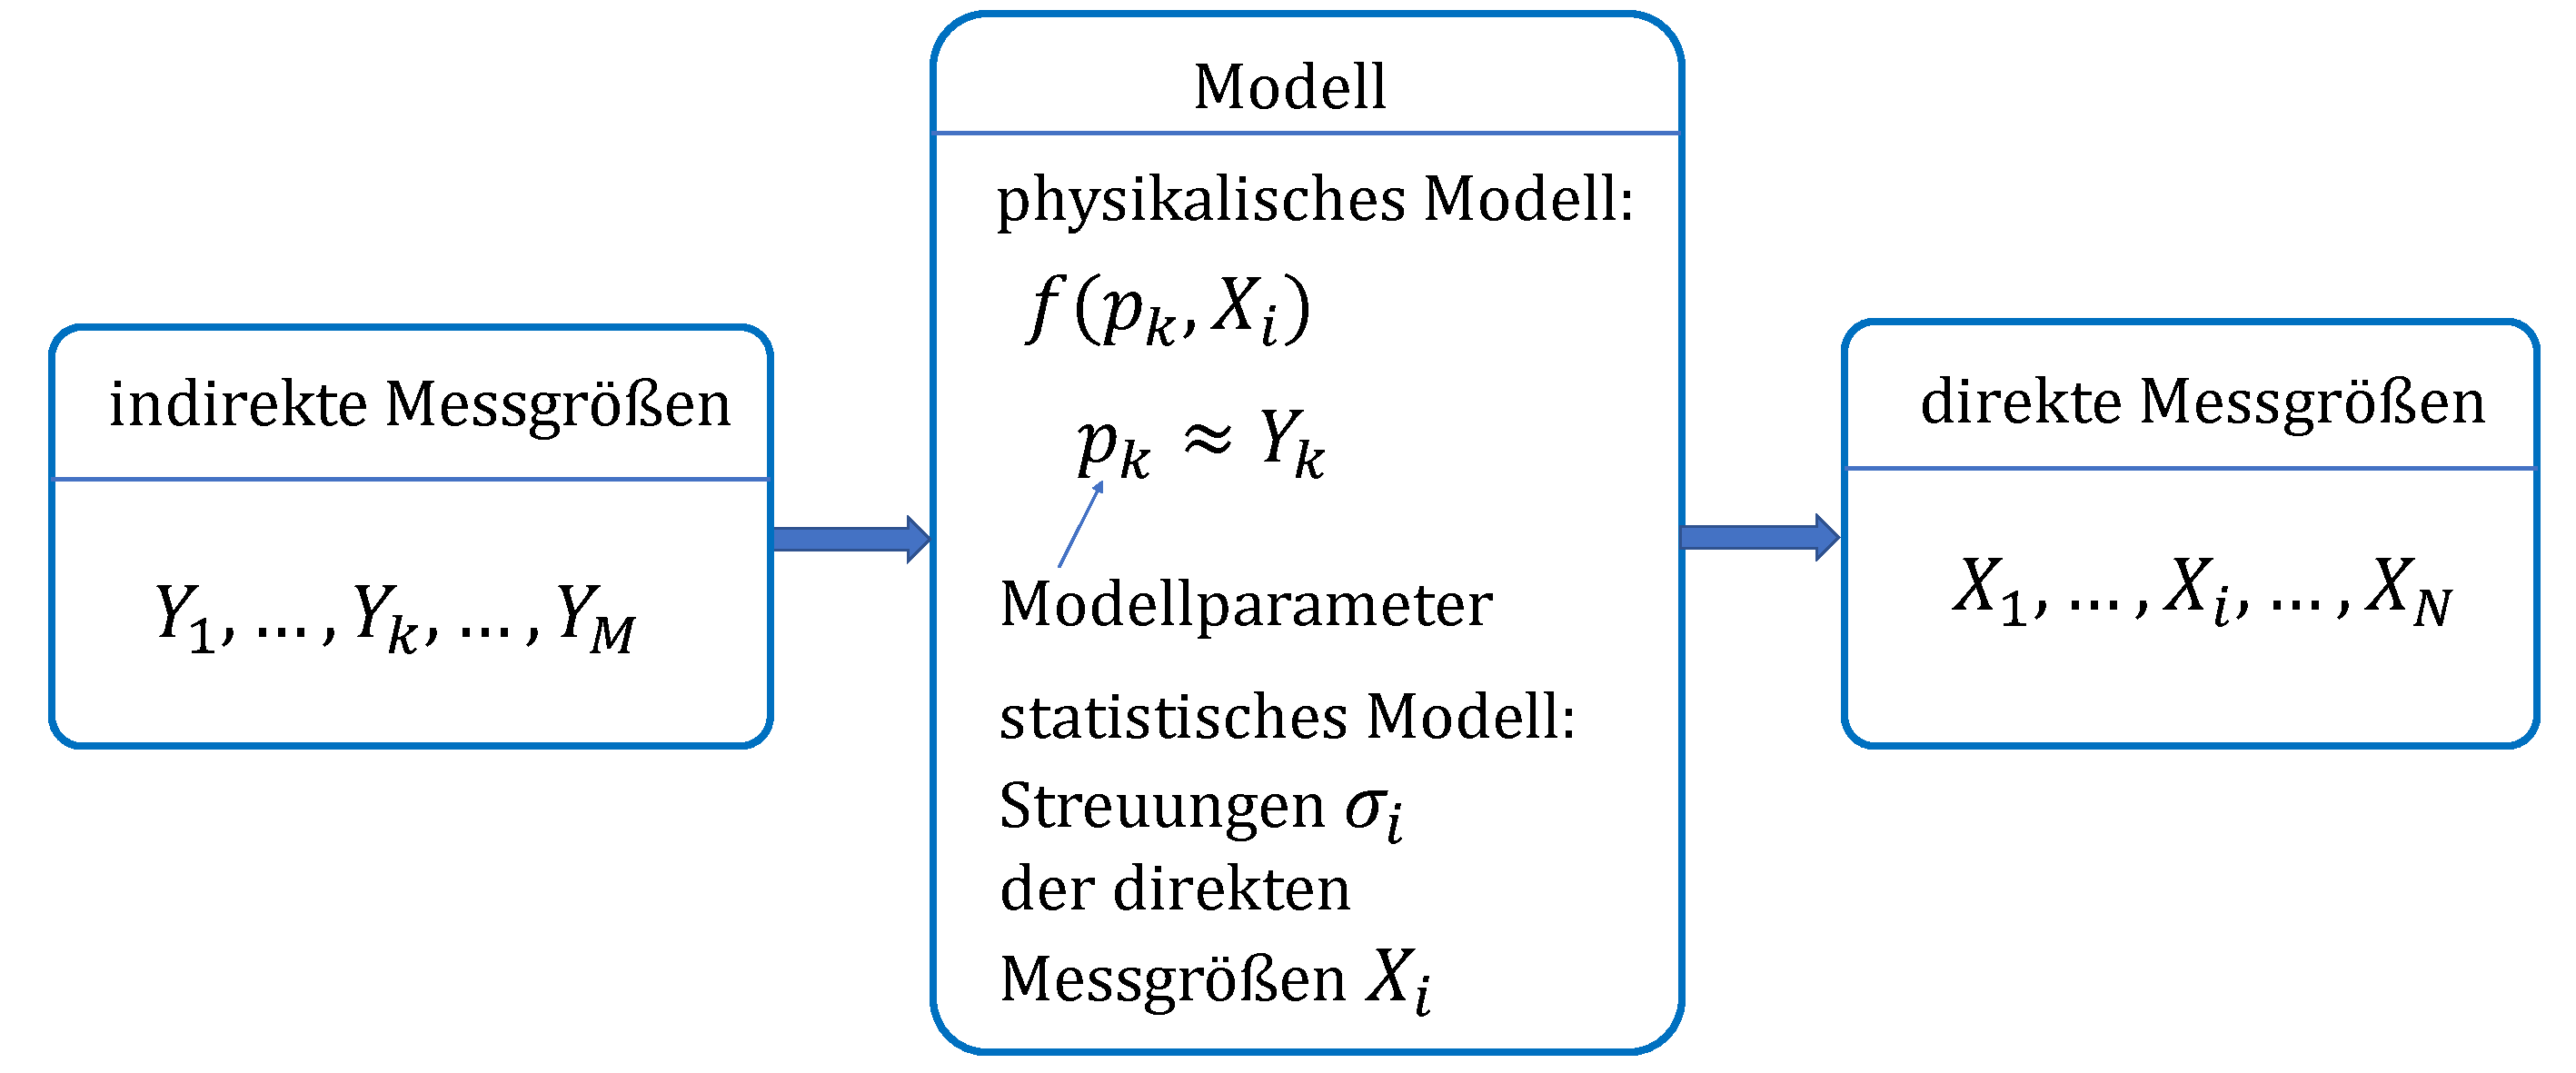
\includegraphics[width=0.8\textwidth, angle = 0]{02_vorlesung/media/Vorl3_Modell1.pdf}
\end{center}
\caption{Modellbildung zur Gewinnung indirekter Messgrößen aus direkten Messgrößen}
\end{figure}

Ein Messvorgang liefert Beobachtungen zu den direkten Messgrößen.
Die wahren Werte der indirekten Größen bleiben verborgen. Die
indirekten Größen können nur geschätzt werden, oftmals auch nur approximiert werden,
weil die Modelle den physikalischen Sachverhalt nur annähernd beschreiben;
denn die Realität ist deutlich komplexer und wird von vielfältigen Einflussfaktoren
bestimmt. Die approximierenden und zufällig streuenden Größen, die die indirekten Messgrößen
repräsentieren, nennen wir \textsl{Modellparameter}.
Die Abweichungen der Modellparameter entstehen also zum einen
durch vereinfachende Modellannahmen und zum anderen durch zufällige Einflüsse wie das
thermische Rauschen von Elektronik oder Vibrationen im Laborraum.

Als gemeinsamen Bezeichner für Modellparameter wählen wir im folgenden
$\mathbf{p} = (P_1, \dots, P_M)$.
Der Buchstabe $\mathbf{p}$ steht hier einfach nur für den Anfangbuchstaben
von dem Begriff Parameter und der Fettdruck weist darauf hin, dass es ein Vektor mit vielen
Einzelparametern sein kann und dient ferner dazu, das Symbol von dem für die Wahrscheinlichkeitsdichte
zu unterscheiden. Diese wird mit $p$ für den Anfangsbuchstaben von \textsl{probability} bezeichnet.
Für die einzelnen Parameter $P_m$ haben wir den Großbuchstaben gewählt, um die Unterscheidung zur
Wahrscheinlichkeitsdichtefunktion zu haben, sowie in Anlehnung an die Konvention Großbuchstaben
$X_i$ und $Y_m$ für die Messgrößen zu verwenden.
\begin{equation}
P_1 \approx Y_1, \dots, P_M \approx Y_M
\end{equation}
Der Schätzvorgang wird als \textsl{Lösen eines inversen Problems} interpretiert.
\begin{equation}
(X_1, \dots, X_N) \xrightarrow{\mathrm{inverses \; Problem}} (Y_1, \dots, Y_M)
\label{inverseProblem}
\end{equation}

Während der ersten Vorlesung vor zwei Wochen wurde Ihnen das Konzept der
\textsl{Maximum-Likelihood}-Methode vorgestellt, aus
der die Methode der kleinsten Residuenquadratsumme hervorgeht. Die Wahrscheinlichkeit,
dass ein Messwert um den Wert $\varepsilon$ von dem geschätzten Modell abweicht, folgt
einer Normalverteilung. Mit anderen Worten kann man auch sagen, dass
die Verteilung der Residuen eine Gaußverteilung ist.
Die Begriffe Gaußverteilung und Normalverteilung verwenden wir synonym.
\begin{equation}
p(\varepsilon | \theta_1,\dots,\theta_M, \sigma) \; = \; \frac{1}{\sigma \sqrt{2 \pi}}
e^{-\frac{1}{2} \left(\frac{\varepsilon}{\sigma}\right)^2}
\label{Maximumlikelihood1}
\end{equation}
Die Symbolik $p(\varepsilon | \theta_1,\dots,\theta_M, \sigma)$ wird gesprochen:
\begin{quote}
Wahrscheinlichkeit $p$ des Eintretens des Ereignises $\varepsilon$
gegeben die Parameter $\theta_1,\dots,\theta_M$ und $\sigma$.
\end{quote}
Der Sprachgebrauch \glqq Eintretens des Ereignises $\varepsilon$\grqq ~stellt die
Sprechweise der Statistik dar. In den angewandten Wissenschaften, Messtechnik,
Elektrotechnik, etc.\ spricht man von der Wahrscheinlichkeit, dass die Messgröße
oder hier die Abweichung der Messgröße vom Modell einen Wert $\varepsilon$ annimmt.

Vor einer Woche wurden Sie mit der Regressionsrechnung vertraut gemacht, die
eine spezielle Anwendung der Maximum-Likelihood-Methode darstellt, bei der
Größen beteiligt sind, die keine Zufallsgrößen darstellen, die Regressoren.
Die Residuen und entsprechend die Regressanden sind die Zufallsgrößen,
für die die in Gl.~(\ref{Maximumlikelihood1}) formulierte Wahrscheinlichkeitsdichte
angenommen wird.
Diese Modellannahme, dass die \textsl{Residuen} als normalverteilt angenommen werden,
hatten wir Vorl.~2 wie folgt formuliert:
\begin{quote}
Die abhängigen Größen $Y$, d.h.\ die \textsl{Regressanden} streuen und ihre Residuen sind
	normalverteilt mit Erwartungswert $E(\varepsilon) = 0$ und Varianz $\mathrm{Var}(\varepsilon) = \sigma^2$. 
	Die Residuen sind \textsl{unabhängig und identisch verteilt}, kurz u.i.v.
	\begin{equation}
	\varepsilon \; \overset{u.i.v.}{\sim} \; \mathcal{N}(0,\sigma) .
	\label{Resinormalverteilt}
	\end{equation}
\end{quote}
Ein Residuum der linearen Regression mit $Y$ als Regressand und $X$ als Regressoren
hat folgende Gestalt
\begin{equation}
\varepsilon_j \; = \; Y_j \; - \; \sum\limits_{i=1}^{M} \theta_i \, X_{i,j}
\end{equation}
wobei der Bezeichner $Y$ der Regressionsrechnung die direkte Messgröße ist und die
Regressoren ebenfalls zu den direkten Größen gehören, jedoch nicht als Zufallsgrößen mit
Streuung, sondern mit vorgegebenen, deterministischen Werten.

Ein Residuum nach der Methode der kleinsten Quadrate für ein Modell mit genau nur einer
einzigen Zufallsgröße $X$ mit einem Modellparameter $\mu$ ist einfach
\begin{equation}
\varepsilon_j \; = \; X_j \, - \, \mu .
\label{oneQuantityOnly1}
\end{equation}

Ein Residuum nach der Methode der kleinsten Quadrate für ein Modell ohne Regressoren,
also mit allen beteiligten Größen als Zufallsgrößen, lässt sich allgemein nicht mit
einem Ansatz darstellen, in dem die Modellparameter linear sind. Bereits bei einer
Geraden, für die sowohl die Abzissengröße $X_1$ als auch die Ordinatengröße $X_2$ streut,
ist der Ansatz nichtlinear. Der Modellparameter Steigung der Geraden ist der Tangenz des
Winkels $\alpha$ der Geraden relativ zur Abzisse. Der zweite Modellparameter
ist der Abstand $d$ der Geraden vom Koordinatenursprung. Das Residuum $\varepsilon_j$ stellt den
Abstand des $j$-ten Messpunktes $(X_{1,j}, X_{2,j})$ zum Modell dar, siehe Abb.~\ref{ResiduenVarianzen}.
\begin{equation}
\varepsilon_j \; = \; 
\left(\begin{array}{c} X_{1,j}\\ X_{2,j}\end{array}\right) \cdot
\left(\begin{array}{c} -\sin(\alpha)\\ \cos(\alpha)\end{array}\right) \; - \; d .
\label{TLSgerade}
\end{equation}
Bei der Lösung von inversen Problemen, bei denen im Gegensatz zur linearen
Regression eine nichtlineare Verknüpfung der Modellparameter vorliegt, lassen
sich die Parameter nicht mehr durch Lösen eines linearen Gleichungssystems bestimmen.
Die Schätzung von Modellparametern besteht dann darin, die Modellparameter auszuprobieren,
d.h.\ viele unterschiedliche Werte vorzugeben, und das Ergebnis der 
Modellrechnungen (\ref{forwardModel2}) mit den beobachteten Werten zu vergleichen, solange,
bis das Ergebnis \glqq gut zu den beobachteten Werten passt\grqq. Numerisch dienen
dazu entsprechende Optimierungsverfahren.
\begin{equation}
(P_1, \dots, P_M) \xrightarrow{\mathrm{Modell}} (X_{\mathrm{Modell},1,j}, \dots, X_{\mathrm{Modell},N,j})
\label{forwardModel2}
\end{equation} 
Im Fall der linearen Regression repäsentiert $\mathbf{p} = (\theta_1,\dots,\theta_M)$,
im Fall der Geraden $\mathbf{p} = (\alpha, d)$ und im Fall der Einzelgröße
$\mathbf{p} = \mu$.

Die beiden Annahmen, dass - wie wir letzte Woche bereits bei der linearen Regression
aufgeschrieben hatten - jede einzelne Beobachtung unabhängig und identisch verteilt 
(u.i.v) ist, sind Voraussetzung der Maximum-Likelihood-Methode:
\begin{itemize}
\item Jeder Messpunkt wurde unabhängig von allen anderen gewonnen.
\item Jeder Messpunkt ist identisch verteilt (sie haben die gleiche Streuung).
\end{itemize}
Die gemeinsame Wahrscheinlichkeitsdichte, engl.\ \textsl{joint probability density}, der
Residuen von $j$ voneinander unabhängigen Messungen ist dann das Produkt der
Wahrscheinlichkeitsdichten $p(\varepsilon_j | \mathbf{p}, \sigma)$
jedes Residuums:
\begin{equation}
p(\varepsilon_1,\dots,\varepsilon_J | \mathbf{p}, \sigma) \; = \; 
\prod\limits_{j = 1}^J \, p(\varepsilon_j | \mathbf{p}, \sigma) \; = \; 
 \frac{1}{(\sigma \sqrt{2 \pi})^J} \prod\limits_{j = 1}^J \, 
e^{-\frac{1}{2} \left(\frac{\varepsilon_j}{\sigma}\right)^2}
\end{equation}
und mit Anwendung des Potenzgesetzes ist dies
\begin{equation}
p(\varepsilon_1,\dots,\varepsilon_J | \mathbf{p}, \sigma) \; = \; 
 \frac{1}{(\sigma \sqrt{2 \pi})^J}  \, 
e^{-\frac{1}{2} \sum\limits_{j = 1}^J \left(\frac{\varepsilon_j}{\sigma}\right)^2} .
\label{Likelihood1}
\end{equation}
Für die Maximum-Likelihood-Methode wird diese Wahrscheinlichkeitsdichte sorum gesehen,
dass die in den Residuen steckenden Beobachtungen vorgegeben sind, und die 
Parameter $\mathbf{p}$ durch Maximieren der Verteilung gesucht wird und sich daraus
die Streuung der Residuen $\sigma$ ergibt. Die Residuen sind Funktion der
Beobachtungen $X_{1,j},\dots,X_{N,j}$ und der Parameter $\mathbf{p}$, also
$\varepsilon_j = \varepsilon(X_{1,j},\dots,X_{N,j}, \mathbf{p})$. 
Deshalb formulieren wir die Wahrscheinlichkeitsdichte
$p(\varepsilon_1,\dots,\varepsilon_J | \mathbf{p}, \sigma)$ 
als \textsl{Likelihood} \\
$l(\mathbf{p}, \sigma | \{X_{1,1}, \dots, X_{1,J}\}, \dots, \{X_{N,1}, \dots, X_{N,J}\})$
um und Gl.~(\ref{Likelihood1}) formen wir damit wie folgt um zu
\begin{equation}
l(\mathbf{p}, \sigma | \{X_{1,1}, \dots, X_{1,J}\}, \dots, \{X_{N,1}, \dots, X_{N,J}\}) \; = \; 
 \frac{1}{(\sigma \sqrt{2 \pi})^J}  \, 
e^{-\frac{1}{2} \sum\limits_{j = 1}^J \left(\frac{\varepsilon(X_{1,j},\dots,X_{N,j}, \mathbf{p})}{\sigma}\right)^2} .
\label{Likelihood2}
\end{equation}

Die Maximum-Likelihood-Methode bedeutet: Finde derartige Parameter $\mathbf{p}$, für die
die \textsl{Likelihood} maximal wird
\begin{equation}
\max_{\mathbf{p}} \, \left\{ l(\mathbf{p}) \right\}.
\end{equation}
Wir maximieren die in Gl.~(\ref{Likelihood2}) gegebene \textsl{Likelihood}, indem wir
ihren Exponenten minimieren
\begin{equation}
\min_{\mathbf{p}}\left\{ \sum\limits_{j = 1}^J \left(\frac{\varepsilon(X_{1,j},\dots,X_{N,j},\mathbf{p})}{\sigma}\right)^2  \right\}.
\end{equation}
Hierbei fällt die Varianz, die für alle Residuen und Parameter denselben Wert hat, raus und
das Optimierungsproblem, d.h.\ die Suche des Minimums, reduziert sich
auf das Variieren der Parameter $\mathbf{p}$
\begin{equation}
\min_{\mathbf{p}} \left\{ \sum\limits_{j = 1}^J \, \varepsilon(X_{1,j},\dots,X_{N,j},\mathbf{p})^2  \right\} .
\end{equation}

Die Aussage, dass jeder Messpunkt identisch verteilt ist, also die gleiche Streuverteilung hat,
bedeutet aber nicht unbedingt, dass die Streubreite eine skalare Größe $\sigma$ sein muss,
sondern nur, dass für alle Beobachtungen die identischen Varianzen gelten.

Wenn der Messpunkt wie in Gl.~(\ref{TLSgerade}) ein Vektor aus zwei Größen ist, die nicht
dieselbe physikalische Dimension haben oder zwar dieselbe physikalische Dimension, aber dennoch
unterschiedliche stark streuen, weil die Messprinzipien sich unterscheiden, dann stellt sich
die Darstellung der Residuen komplizierter dar. Ein Beispiel für unterschiedliche physikalische
Dimensionen kann wieder das mit der Messung eines elektrischen Widerstandes sein, bei dem $X_1$ eine
Strommessung und $X_2$ eine Spannungsmessung repräsentieren kann.
Ein Beispiel für dieselbe physikalische Dimension mit unterschiedlichem Streuverhalten kann ein
Oberflächenmessgerät sein, bei dem die Sensorik in vertikaler Richtung zur Messung der Höhen einer
Topographie ein optischer oder taktiler Punktsensor sein kann und die horizontale Achse durch einen
Schlitten mit einem Wegmesssystem in Form eines Glasmaßstabs sein kann.

\begin{figure}
\begin{center}
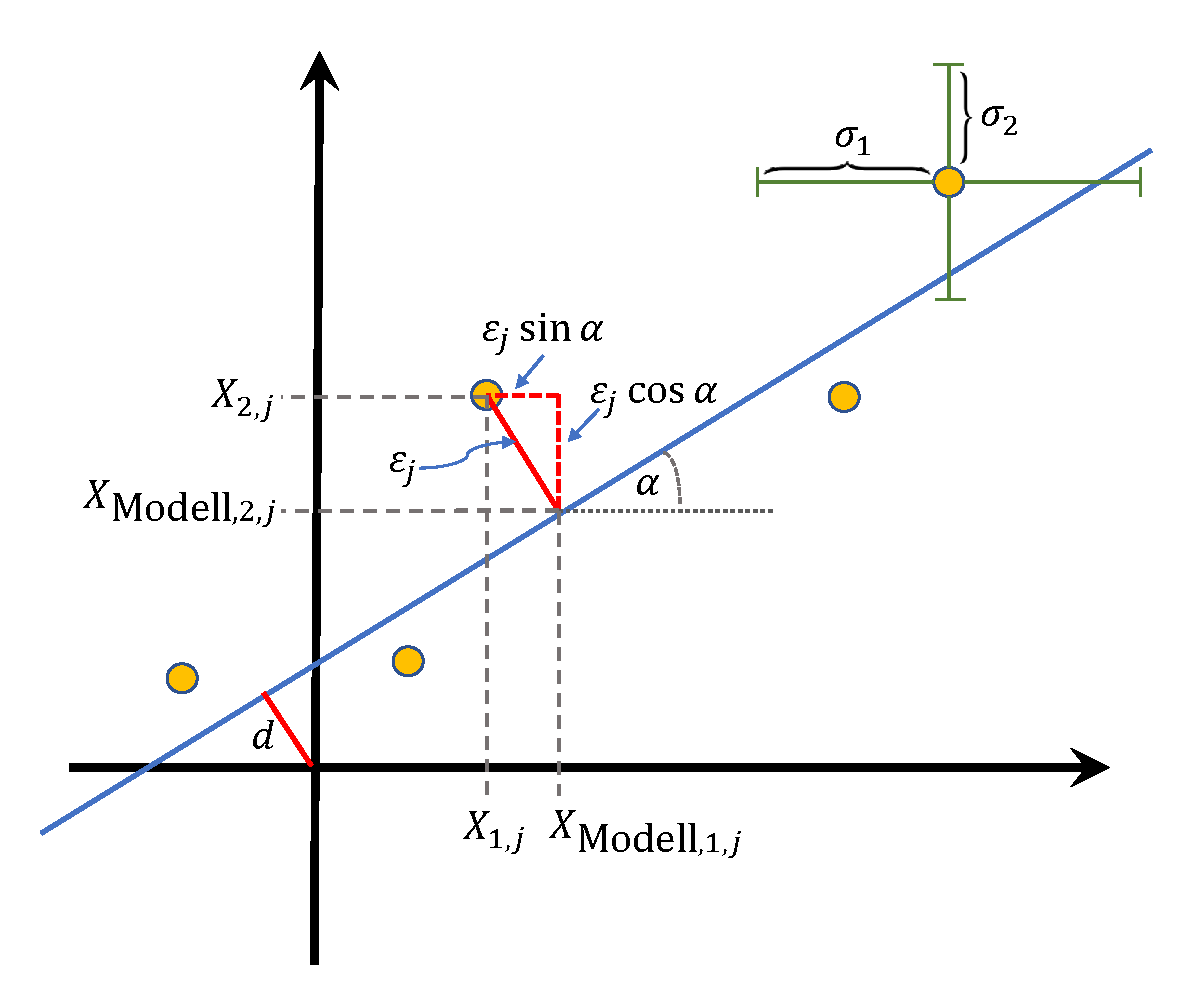
\includegraphics[width=100mm]{02_vorlesung/media/Vorl3_ResiduenVarianzen.pdf}
\end{center}
\caption{Veranschaulichung für Schätzung von Geradenparametern durch
Minimierung der Summe der Quadrate der Residuen bei verschiedenen Varianzen 
$\sigma_1^2$ und $\sigma_2^2$ der beiden direkten Messgrößen $X_1$ und $X_2$
\label{ResiduenVarianzen}}
\end{figure}
Angenommen Größe $X_1$ zu Gl.~(\ref{TLSgerade}) streue normalverteilt mit $\sigma_1$ und
$X_2$ mit $\sigma_2$, so müsste man beispielsweise die Residuen aus Gl.~(\ref{TLSgerade}) in
Vektorkomponenten parallel zu den die beiden Größen repäsentierenden Achsen zerlegen
\begin{equation}
\vec \varepsilon_j \; = \;
\left(\begin{array}{c}
-\varepsilon_j \sin(\alpha)\\
\varepsilon_j \cos(\alpha)
\end{array}\right) ,
\end{equation}
so dass wir für die Wahrscheinlichkeitsdichte
der $j$-ten Beobachtung den verschiedenen Streubreiten Rechnung tragen können:
\begin{equation}
p(\varepsilon_j | \alpha, d, \sigma_1, \sigma_2) \; \propto \; 
e^{-\frac{1}{2} \left(\frac{\varepsilon_j \sin(\alpha)}{\sigma_1}\right)^2}
\, e^{-\frac{1}{2} \left(\frac{\varepsilon_j \cos(\alpha)}{\sigma_2}\right)^2}
\end{equation}
In der Literatur werden zur Anpassung einer Geraden an zwei Größen
unterschiedlicher Varianz sehr verschiedene Ansätze und Methoden vorgeschlagen.

Die Abweichungen der direkten Messgrößen zu den entsprechenden Werten, also die Residuen,
die bei der Modellschätzung Gl.~(\ref{forwardModel2}) errechnet werden, müssen als
vektorielle Größen behandelt werden, wenn die verschiedenen direkten Messgrößen $X_i$ eine
unterschiedliche Varianz $\sigma_i^2 = \sigma_{i,i}$ oder noch allgemeiner auch
Kovarianzen $\sigma_{i,k}$ aufweisen, die als Kovarianzmatrix
\begin{equation}
\boldsymbol{\Sigma} \; = \;
\left(\begin{array}{ccc}
\sigma_1^2 & \dots & \sigma_{1,N}\\
 & \ddots & \\
\sigma_{N,1} & \dots & \sigma_N^2
\end{array}\right)
\end{equation}
zusammengefasst wird.

Die Wahrscheinlichkeitsdichteverteilung für den Vektor der Residuen der
$j$-ten Beobachtung ist dann
\begin{equation}
p(\vec \varepsilon_j | \mathbf{p}, \boldsymbol{\Sigma}) \; \propto \; 
e^{-\frac{1}{2} \, \vec \varepsilon^\mathsf{T}_j \, \boldsymbol{\Sigma}^{-1} \, \vec \varepsilon_j }
\end{equation}
wobei
\begin{equation}
\vec \varepsilon_j \; = \; 
\left(\begin{array}{c}
X_{1,j}\\
\vdots\\
X_{N,j}
\end{array}\right) \, - \, 
\left(\begin{array}{c}
X_{\mathrm{Modell},1,j}\\
\vdots \\
X_{\mathrm{Modell},N,j}
\end{array}\right) .
\label{Residuen}
\end{equation}
Die \textsl{joined probability density} ist dann entsprechend
\begin{equation}
p(\vec \varepsilon_1,\dots, \vec \varepsilon_J | \mathbf{p}, \boldsymbol{\Sigma}) \; \propto \; 
\prod\limits_{j=1}^J \,
e^{-\frac{1}{2} \, \vec \varepsilon^\mathsf{T}_j \, \boldsymbol{\Sigma}^{-1} \, \vec \varepsilon_j } \; = \;
e^{-\frac{1}{2} \; \sum\limits_{j=1}^J \, \vec \varepsilon^\mathsf{T}_j \, \boldsymbol{\Sigma}^{-1} \, \vec \varepsilon_j } .
\label{LikelihoodKov}
\end{equation}


Für die Lösung eines inversen Problems geht es darum, die Parameter $\mathbf{p}$
für gegebene Beobachtungen $X_{i,j}$ zu finden, die die Wahrscheinlichkeitsdichte
in Gl.~(\ref{LikelihoodKov}) maximieren. Wir schreiben deshalb die Residuenvektoren $\vec \varepsilon_j$ als Funktion
der Beobachtungen $\vec \varepsilon(X_{1,j},\dots,X_{N,j},\mathbf{p})$ auf und verändern die Schreibweise
für die Wahrscheinlichkeit so, dass wir als Likelihood $l$, die eine Funktion der
Variablen $\mathbf{p}$ und $\boldsymbol{\Sigma}$ für gegebene Beobachtungen $(X_{1,j},\dots,X_{N,j})$ ist,
ausdrücken. Gl.~(\ref{LikelihoodKov}) bekommt dann folgende Gestalt
\begin{equation}
l(\mathbf{p}, \boldsymbol{\Sigma} | \{X_{1,1}, \dots, X_{1,J}\}, \dots, \{X_{N,1}, \dots, X_{N,J}\} ) \; \propto \; 
e^{-\frac{1}{2} \; \sum\limits_{j=1}^J \, \vec \varepsilon^\mathsf{T}(X_{1,j},\dots,X_{N,j},\mathbf{p}) \, \boldsymbol{\Sigma}^{-1} \, \vec \varepsilon(X_{1,j},\dots,X_{N,j},\mathbf{p}) } .
\label{LikelihoodKov2}
\end{equation}
Die Kovarianzmatrix ist wie die Residuen Funktion der Parameter und der Beobachtungen,
also $\boldsymbol{\Sigma}(X_{1,j},\dots,X_{N,j},\mathbf{p})$ und
variiert werden die Parameter $\mathbf{p}$.
Zur Maximierung der in Gl.~(\ref{LikelihoodKov2}) gegebenen 
\textsl{Likelihood} wird der Exponent minimiert, was in die Methode der kleinsten Residuenquadratsumme
übergeht, also
\begin{equation}
\min_{\mathbf{p}} \; \left\{ 
 \sum\limits_{j=1}^J \, \vec \varepsilon(X_{1,j},\dots,X_{N,j},\mathbf{p})^\mathsf{T} \, 
\boldsymbol{\Sigma}(X_{1,j},\dots,X_{N,j},\mathbf{p})^{-1} \, \vec \varepsilon(X_{1,j},\dots,X_{N,j},\mathbf{p})_j \right\} .
\label{generalLSmethod}
\end{equation}

\section{Konzept der bayesischen Verfahren zum Lösen inverser Probleme}

Für komplexere Fragestellungen hinsichtlich der Varianzen und hinsichtlich der Möglichkeit,
sukzessive neue Informationen durch weitere Beobachtungen hinzuzufügen und damit die Werte von
interessierenden indirekten Messgrößen immer weiter zu verbessern, stoßen die gängigen Ansätze wie
die Maximum-Likelihood-Methode an gewisse Grenzen. Insbesondere die Möglichkeit, bereits durch
vergangene Optimierungsprozesse gewonnene Parameter durch Gewinnen neuer Beobachtungen zu verändern,
ist nicht Gegenstand der \glqq herkömmlichen\grqq ~Statistik. Mit \glqq herkömmlich\grqq ~ist
an dieser Stelle die \textsl{frequentistische} Statistik gemeint, bei der empirisch aus
Beobachtungen Häufigkeitsverteilungen gewonnen werden, empirische Wahrscheinlichkeitsverteilungen
(Likelihood) berechnet werden, und entsprechend eine Schätzung von Modellparametern erfolgt.
Die lineare Regression ist ein Teilgebiet der \textsl{frequentistischen} Statistik

In der Statistik gibt es dazu zweierlei Blickrichtungen:
\begin{enumerate}
\item In \textbf{frequentistischen Statistik} wird angenommen,
dass der Wert einer indirekten Messgröße unbekannt, aber konstant/ fest ist und deshalb
auch \textsl{wahrer Wert} genannt wird. In Bezug auf die direkt messbaren Größen wird angenommen,
dass sie aufgrund des Mangels an Erkenntnis über alle möglichen Einflüsse und Abläufe im Messprozess
streuen, so dass sie als Zufallsgrößen behandelt werden. Die Behandlung als Zufallsgröße
bedeutet dabei, dass der Wahrscheinlichkeit für eine Beobachtung einen konkreten Wert anzunehmen eine
Wahrscheinlichkeitsdichteverteilung zugrunde gelegt wird.
\begin{equation}
\underbrace{(Y_1, \dots, Y_M)}_{\mathrm{unbek, konst, wahr}} \xrightarrow{\mathrm{Messprozess}}
\underbrace{(X_1, \dots, X_N)}_{\mathrm{Zufallsgroessen}}
\end{equation}
\item Umgekehrt ist die Weise, wie das Zustandekommen der Streuung von Größen gesehen wird,
in der Statistik, die den Satz von Bayes zum Berechnen bedingter Wahrscheinlichkeiten 
verwendet. Dieses Gebiet der Statistik wird wegen der Verwendung des
Satzes von Bayes auch \textbf{bayesische Statistik} genannt.

Hier werden die Beobachtungen der direkten Größen, als konkrete, feste Werte eingesetzt,
um die Erkenntnis über die zu bestimmende indirekte Größe zu überprüfen bzw.\ zu vermehren.
Die Vorstellung ist, dass durch den Mangel an Erkenntnis die indirekten Größen als
Zufallsgrößen zu behandeln sind. Es wird nun also nicht mehr nur eine Likelihood-Verteilung
berechnet, deren Maximum gesucht wird. Sondern es wird eine Kombination der Likelihood mit
einer Wahrscheinlichkeitsdichteverteilung,
die eine {\`a} priori Annahme über die indirekten Messgrößen darstellt, berechnet und der
Erwartungswert (das erste statistische Moment) und die Varianz (das zweite statistische Moment)
dieser kombinierten Verteilungsdichte ermittelt.

Dabei repräsentieren die Wahrscheinlichkeiten für die zu erwartenden Beobachtungen eines Parameters
(einer indirekten Messgröße), 
den Grad der Erkenntnis, vernünftiger Glaubwürdigkeit, über die indirekte Messgröße.
In der englischsprachigen Literatur wird dies \textsl{Degree of Belief} genannt.

Vielleicht kann man sich diese Denkweise so vorstellen wie die Vorgehensweise eines Detektivs
oder Kriminalkommissars beim Sammeln von immer mehr Indizien zum Aufklären eines Falls.
\begin{equation}
\underbrace{(X_1, \dots, X_N)}_{\mathrm{Beobachtungen}} \xrightarrow{\mathrm{inverses \; Problem}}
\underbrace{(Y_1, \dots, Y_M)}_{\mathrm{Zufallsgroessen}} 
\end{equation}
Die Erkenntnis über die indirekten Größen (Modellparameter $Y_1, \dots, Y_M$) wird mit jeder
neuen Messkampagne $\kappa$ revidiert
\begin{equation}
\arraycolsep=2.4pt\def\arraystretch{2}
\left.
\begin{array}{l}
\underbrace{(X_1, \dots, X_N)}_{\mathrm{neue~Beobachtungen}}\\
\underbrace{(Y_1, \dots, Y_M)_{\kappa-1}}_{\mathrm{Zufallsgroessen, vorher}} 
\end{array}\right\}
 \xrightarrow{\mathrm{inverses \; Problem}}
\underbrace{(Y_1, \dots, Y_M)_{\kappa}}_{\mathrm{Zufallsgroessen}} 
\end{equation}
\end{enumerate}
Da wir wie vorher detailiert dargelegt die indirekten Größen durch approximative Modellparameter ersetzten,
also $Y_m \approx P_m$, sind es die Schätzungen zu den Parametern $\mathbf{p} = (P_1,\dots,P_M)$, die
sozusagen \glqq\textsl{upgedated}\grqq ~werden.
\begin{equation}
\arraycolsep=2.4pt\def\arraystretch{2}
\left.
\begin{array}{l}
\underbrace{(X_1, \dots, X_N)}_{\mathrm{neue~Beobachtung}}\\
\underbrace{(P_1, \sigma^2_1, \dots, P_M, \sigma^2_M)_{\kappa-1}}_{\mathrm{Zufallsgroesse, vorher}} 
\end{array}\right\}
 \xrightarrow{\mathrm{inverses \; Problem}}
\underbrace{(P_1, \sigma^2_1, \dots, P_M, \sigma^2_M)_{\kappa}}_{\mathrm{Zufallsgroesse}} 
\end{equation}

Wir betrachten wie in Gl.~(\ref{oneQuantityOnly1}) den einfachsten Fall einer Größe,
die wir wie in Gl.~(\ref{oneQuantityOnly1}) auch hier als Modellparameter $P = \mu$, der
eine indirekte Messgröße $Y$ repräsentieren soll, aufschreiben.
Die Größe $\mu$ ist aus einer Stichprobe zu schätzen.
Als {\`a} priori Information seien folgende Angaben bekannt:
\begin{itemize}
\item Der {\`a} priori Schätzwert der Modellgröße $\mu$ sei $y_0$.
\item Der {\`a} priori Schätzwert seiner Varianz $\sigma^2$ sei $s^2_0$.
\item Diese Größe sei normalverteilt, also verwenden wir als
Verteilungsdichtefunktion $p$ die Gaußverteilung.
\end{itemize}
Die neue Stichprobe $\{X_{1,1}, \dots, X_{1,J}\}$ sei vom Umfang deutlich kleiner, so dass
für die Streuung der Varianz die $\chi^2$-Verteilung $p_{\chi^2,\nu}$
für $\nu = J-1$ Freiheitsgrade verwendet wird. Hierzu müssen wir im Stoff vorgreifen.
Diese Verteilungsdichtefunktion werden wir in der 5.\ Vorlesung behandeln.
Sie wird verwendet als Verteilungsdichte für Varianzen und ist eine schiefsymmetrische
Verteilung mit längerem Ausläufer zu größeren Werten. Je kleiner der Stichprobenumfang,
desto schiefer die Verteilung und ausgeprägter die Ausläufer.

Die gesamte Wahrscheinlichkeitsdichteverteilung $p(Y,\sigma)$ für die indirekte Messgröße
$Y$ bzw.\ deren Approximation als Modellparameter $P = \mu$ mit Streuung $\sigma$ wird als Produkt
folgender Wahrscheinlichkeiten berechnet,
\begin{itemize}
\item der Likelihood $p_\mathrm{L}$, 
\item der Verteilungsdichte $p_\mathcal{N}(y | y_0, s_0)$ der Größe $\mu$ aus den {\`a} priori Informationen,
\item der Verteilungsdichte $p_{\chi^2,\nu}(s)$ der Varianz $\sigma^2$ dieser Größe.
\end{itemize}
Die zu ermittelnde, bedingte Wahrscheinlichkeitsdichte wird so interpretiert, dass die Verteilung Funktion
der Variablen $\mu$ und $\sigma$ ist, gegeben die Beobachtungswerte der Stichprobe. Die Likelihood wird
dabei betrachtet als die bedingte Wahrscheinlichkeitsdichte $p_\mathrm{L}$ der
direkten Messgröße $X_1$ gegeben die Modellparameter $\mu$ und $\sigma$:
\begin{equation}
p_\mathrm{L}(\{X_{1,1}, \dots, X_{1,J}\} | \mu, \sigma) \; = \;
\prod\limits_{j=1}^J \frac{1}{\sqrt{2 \pi} \, \sigma}
 e^{- \frac{1}{2} \, \left( \frac{X_{1,j} - \mu}{\sigma} \right)^2 }  \; = \;
l(\mu, \sigma | \{X_{1,1}, \dots, X_{1,J}\}).
\end{equation}
Die Varianz $\sigma^2$ wird gemäß der $\chi^2$-Verteilung variert. Das Variieren der Varianz
bzw.\ deren Wurzel $\sigma$ symbolisieren wir durch den Gebrauch der Variablen $s$.
Das Variieren des Modellparameters $\mu$ symbolisieren wir durch den Gebrauch der Variablen $y$.
Der Parameter $\mu$ wird ebenfalls variiert gemäß der Gaußverteilung, wir verwenden folgende
Likelihood:
\begin{equation}
p_\mathrm{L}(\{X_{1,1}, \dots, X_{1,J}\} | y, s) \; = \;
\prod\limits_{j=1}^J \frac{1}{\sqrt{2 \pi} \, s}
 e^{- \frac{1}{2} \, \left( \frac{X_{1,j} - y}{s} \right)^2 }  \; = \;
l(y, s | \{X_{1,1}, \dots, X_{1,J}\}).
\end{equation}

\begin{figure}
\begin{center}
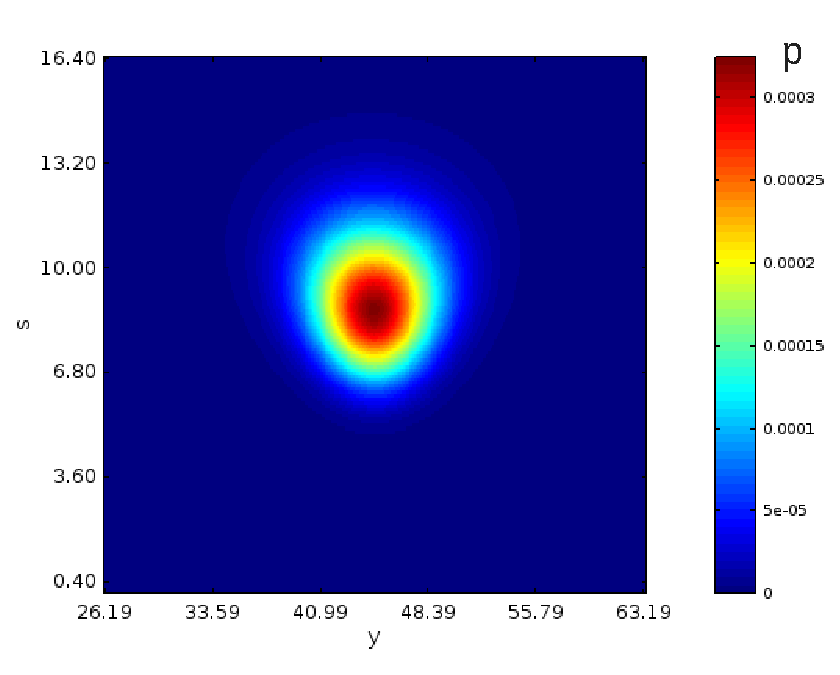
\includegraphics[width=100mm]{02_vorlesung/media/understand_bayes_mean_posteriormatrix.pdf}
\caption{\label{posteriormatrix} Posterior-Wahrscheinlichkeitsdichte als Funktion
der beiden zu schätzenden Größen $y$ und $s$.}
\end{center}
\end{figure}
Das Produkt ist die Wahrscheinlichkeit des Modellparameters und dessen Varianz gegeben
die Stichprobe $\{X_{1,1}, \dots, X_{1,J}\}$ und die {\`a} priori Informationen $y_0, s_0$
\begin{equation}
p(y, s | \{X_{1,1}, \dots, X_{1,J}\}, y_0, s_0) \; = \; C \,
p_\mathrm{L}(\{X_{1,1}, \dots, X_{1,J}\} | y, s) \; p_\mathcal{N}(y | y_0, s_0) \; p_{\chi^2,\nu}(s)
\label{ProduktWahrscheinlichkeiten}
\end{equation}
mit $C$ als Normierungsfaktor derart zu wählen, dass die integrierte Wahrscheinlichkeit Eins ist, d.h.
$$
\int\limits_{-\infty}^\infty  \int\limits_0^\infty \; p(y, s | \{X_{1,1}, \dots, X_{1,J}\}, y_0, s_0) \;
\operatorname{d}s \, \operatorname{d}y \; = \; 1 .
$$
Die Verteilungsdichte $p(y, s | \{X_{1,1}, \dots, X_{1,J}\}, y_0, s_0)$ ist Funktion der
Variablen $y$ und $s$ mit vorgegebenen Parametern 
(festen Werten) $\{X_{1,1}, \dots, X_{1,J}\}$, $y_0, s_0$, wie es beispielhaft in 
Abb.~\ref{posteriormatrix} dargestellt wird.

Die Wahrscheinlichkeitsdichteverteilung
$p_\mathcal{N}(y | y_0, s_0)$ wird \textsl{Prior} genannt und die
Wahr\-schein\-lich\-keits\-dichte\-ver\-teilung $p(y, s | \{X_{1,1}, \dots, X_{1,J}\}, y_0, s_0)$
wird \textsl{Posterior} genannt.

Wir integrieren Gl.~(\ref{ProduktWahrscheinlichkeiten}) über $s$ um eine 
Wahrscheinlichkeits\-dichte\-verteilung zu gewinnen, die nur noch Funktion von $y$ ist
\begin{equation}
p(y | \{X_{1,1}, \dots, X_{1,J}\}, y_0, s_0)  \; = \;
\int\limits_0^\infty p(y, s | \{X_{1,1}, \dots, X_{1,J}\}, y_0, s_0) \operatorname{d}s
\label{RandverteilungPosterior}
\end{equation}
Diese Verteilung wird \textsl{Randverteilung} oder \textsl{Marginalverteilung} genannt.
Allgemeiner gilt: Gegeben zwei Zufallsgrößen $A$ und $B$ mit gemeinsamer Verteilungsdichte
$p(A, B)$ dann heißen die Verteilungen der einzelnen Zufallsgrößen
$A$ und $B$ die Randverteilungen des Zufallsvektors $(A, B)$.

Als Schätzwert für $Y$ berechnen wir den Erwartungswert des Modellparameters $\mu$
durch Integration über alle Werte $y$ gewichtet mit der Wahrscheinlichkeitsdichte\\
$p(y | \{X_{1,1}, \dots, X_{1,J}\}, y_0, s_0)$ aus Gl.~(\ref{RandverteilungPosterior})
\begin{equation}
y_1 \; = \; \int\limits_{-\infty}^\infty \, y \, p(y | \{X_{1,1}, \dots, X_{1,J}\}, y_0, s_0) 
\operatorname{d}y
\end{equation}
wobei wir $y_1$ mit Index $1$ schreiben, um anzuzeigen, dass dies die Revision der Schätzung des 
Modellparameters $\mu \approx Y$ gegenüber vorheriger Kenntnis mit Schätzwert $y_0$ ist.

Zu einem \textsl{Messergebnis} gehört jeweils ein Intervall, das ein Maß für die Unsicherheit
des Wertes/ der Werte der Messgröße ist, siehe [VIM 2.9]

\begin{quote}
\textbf{Messergebnis}

Menge von Größenwerten, die einer Messgröße zugewiesen sind, zusammen mit jeglicher
verfügbarer relevanter Information

ANMERKUNG 1 Ein \textsl{Messergebnis} enthält im Allgemeinen \glqq relevante Information\grqq ~über
die Menge der Größenwerte, von denen einige repräsentativer für die Messgröße sein können als andere.
Dies kann in Form einer Wahrscheinlichkeitsdichtefunktion ausgedrückt werden.

ANMERKUNG 2 Ein \textsl{Messergebnis} wird im Allgemeinen
als ein einziger Messwert und eine \textsl{Messunsicherheit}
ausgedrückt. Wird die Messunsicherheit für einige
Zwecke als vernachlässigbar angesehen, kann das
Messergebnis als ein einziger Messwert ausgedrückt
werden. In vielen Bereichen ist dies die übliche Art, ein
Messergebnis auszudrücken.

ANMERKUNG 3 In der traditionellen Literatur und in der
vorhergehenden Ausgabe des VIM war das Messergebnis
als ein Wert definiert, der einer Messgröße zugewiesen
ist, und so erklärt, dass er eine Anzeige oder ein
unkorrigiertes oder ein korrigiertes Ergebnis bedeutet, je
nach Kontext.
\end{quote}

Mit der in Anmerkung~1 angesprochenen Wahrscheinlichkeitsdichtefunktion sind Verteilungen wie
die in den Gln.~(\ref{Likelihood2}) und (\ref{LikelihoodKov2}) vorgestellen Likelihoods oder
der in Gl.~(\ref{RandverteilungPosterior}) vorgestellten Posterior
mit $p(y | \{X_{1,1}, \dots, X_{1,J}\}, y_0, s_0)$ gemeint. Die Likelihood wird
für kleine Stich\-proben\-um\-fänge ($N < 100$) anstelle durch eine Gaußverteilung durch eine Verteilung 
repräsentiert, deren Charakteristik im Kurvenverlauf
überhöhter und mit länger auslaufenden Rändern ist. Sie wird $t$-Verteilung genannt.
Wir werden später in der 5.\ Vorlesung auf diesen Verteilungtyp zurück kommen.

Allgemein betrachten wir für beide Fälle eine Wahrscheinlichkeitsdichtefunktion $p \! : y \mapsto p(y)$.
Der Definitionsbereich für $y$ reicht von minus bis plus Unendlich reicht. Von Interesse ist der Kernbereich
der Dichteverteilung für eine spezifizierte Wahrscheinlichkeit $1-\alpha$, beispielsweise
$1-\alpha = 0.95$ oder $0.90$ oder so.
Dies ist die Wahrscheinlichkeit einer Größe, einen Messwert im Bereich (Intervall) $[y_\mathrm{min}, y_\mathrm{max}]$,
anzunehmen
\begin{equation}
1 \, - \, \alpha \; = \; 
\int\limits_{y_\mathrm{min}}^{y_\mathrm{max}} p(y) 
\operatorname{d}y .
\label{UeberdeckungWahrscheinlichkeit}
\end{equation}
Die Breite des Intervalls gibt dann die \textsl{Messunsicherheit} an.

Das Intervall $[y_\mathrm{min}, y_\mathrm{max}]$, zu dem die Fläche $1 - \alpha$ unter der die
Verteilungsdichte $p(y)$ repräsentierenden Kurve gehört, wird \textsl{Überdeckungsintervall} genannt.
Es ist der verallgemeinerte Begriff aus der Metrologie für das, was in der
\textsl{frequentistischen} Statistik \textsl{Vertrauensintervall},
engl.\  \textsl{Confidence Interval}, und in der \textsl{bayesischen} Statistik 
\textsl{Glaubwürdigkeitsintervall}, engl.\ \textsl{Credible Interval},
heißt. Während der Begriff \textsl{Vertrauensintervall} in der deutschsprachigen
Literatur üblich ist, wird anstelle des Begriffs \textsl{Glaubwürdigkeitsintervall} üblicherweise
auch in der deutschsprachigen Literatur der Begriff \textsl{Credible Interval} verwendet.

Die Verwendung unterschiedlicher Bezeichnungen, \textsl{Confidence Interval} und
\textsl{Credible Interval}, sollen die Unterschiedlichkeit der Vorstellungen
über den Charakter einer indirekten Messgröße $Y$ zum Ausdruck bringen.
Die Unterschiedlichkeit in der Vorstellung von einer indirekten Messgröße $Y$ besteht darin,
dass im Fall der \textsl{bayesischen} Statistik
die indirekte Messgröße $Y$ als Größe, die intrinsisch eine Zufallsgröße ist, betrachtet
wird. Im Fall der \textsl{frequentistischen} Statistik wird $Y$ als eine Größe betrachtet,
die einen festen, wahren Wert hat, der aber nicht zugänglich ist. Nur der
Modellparameter, der eine indirekte Messgröße approximiert und der indirekt aus anderen 
Zufallsgrößen gewonnen wird, wird als daraus resultierend einer Streuung unterliegend betrachtet.

Die Wahrscheinlichkeit $1 - \alpha$ wird in der \textsl{frequentistischen} Statistik
\textsl{Vertrauensniveau} genannt. Die beiden Flächen unter den
Ausläufern der Dichteverteilung stellt eine Wahrscheinlichkeit $\alpha$ dar, die in der
\textsl{frequentistischen} Statistik \textsl{Signifikanzniveau} genannt wird.

Im folgenden werden wir sehen, wie eine \textsl{Messunsicherheit} im Rahmen der
\textsl{bayesischen} Statistik gewonnen wird.
Die Grenzen des \textsl{Credible Interval} $[y_\mathrm{min}, y_\mathrm{max}]$ bilden die
Integrationsgrenzen $y_\mathrm{min}$ und $y_\mathrm{max}$ der \textsl{Posterior}, so dass
\begin{equation}
1 \, - \, \alpha \; = \; 
\int\limits_{y_\mathrm{min}}^{y_\mathrm{max}} p(y | \{X_{1,1}, \dots, X_{1,J}\}, y_0, s_0) 
\operatorname{d}y .
\label{UeberdeckungPosterior}
\end{equation}
Die Integrationsgrenzen werden über die Umkehrfunktion der kumulativen Verteilung $P$ berechnet.
Die kumulative Verteilung $P$ ist
\begin{equation}
P(y) \; = \; \int\limits_{-\infty}^{y} p(y^\prime | \{X_{1,1}, \dots, X_{1,J}\}, y_0, s_0) 
\operatorname{d}y^\prime .
\end{equation}
Die Umkehrfunktion schreiben wir symbolisch als $P^{-1}$.
Wir berechnen für das \textsl{Credible Interval}
\begin{equation}
y_\mathrm{min} \, = \, P^{-1}(\frac{\alpha}{2}) \qquad \mathrm{und} \qquad
y_\mathrm{max} \, = \, P^{-1}(\frac{1-\alpha}{2}).
\end{equation}
\begin{figure}
\begin{center}
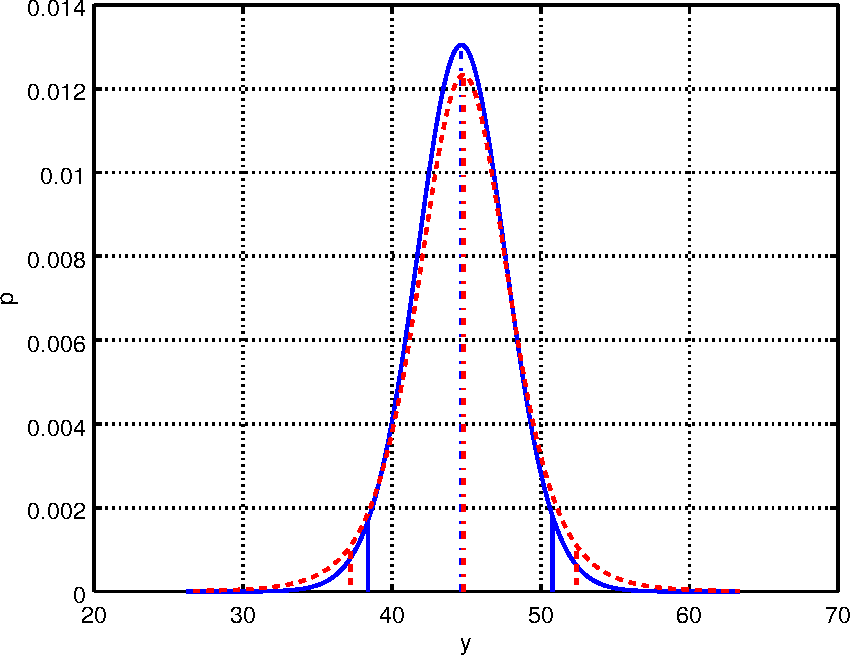
\includegraphics[width=80mm]{02_vorlesung/media/understand_bayes_mean_posteriormarginal.pdf}
\hspace{5mm}
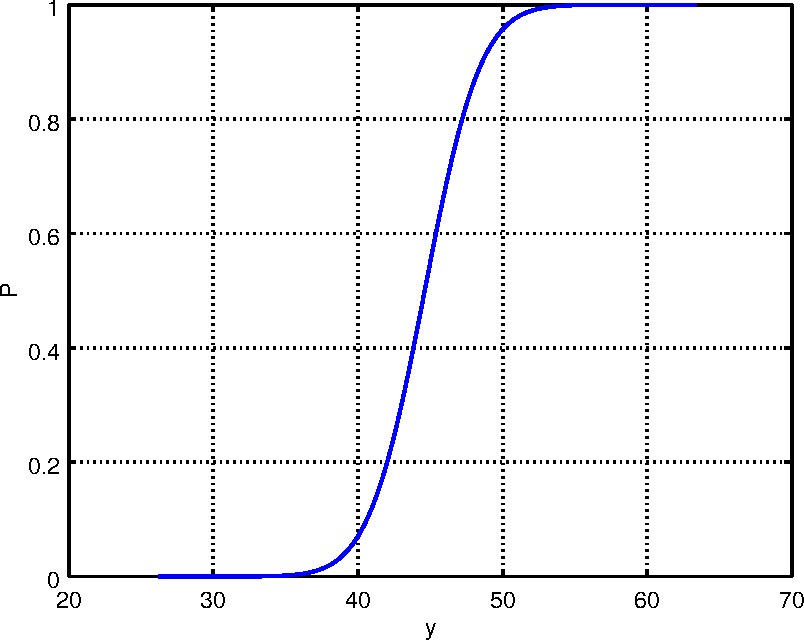
\includegraphics[width=80mm]{02_vorlesung/media/understand_bayes_mean_cumposterior.pdf}
\caption{\label{posteriorCredible}\textsl{Links:} Die blaue Kurve stellt die
Randverteilung der Posterior-Wahrscheinlichkeitsdichte als Funktion
der beiden zu schätzenden Größen $Y$ mit \textsl{Credible Interval} dar und die
rot gestrichelte Kurve die Student-t-Verteilung mit Vertrauensintervall.
\textsl{Rechts:} Kumulierte Randverteilung der Posterior-Wahrscheinlichkeitsdichte, deren
Umkehrfunktion verwendet wird, um die Intervallgrenzen des \textsl{Credible Interval}s zu ermitteln.}
\end{center}
\end{figure}
Abb.~\ref{posteriorCredible} links zeigt im Vergleich folgende Verteilungsdichten
\begin{itemize}
\item die Posterior als Funktion des Parameters
$y$ mit einem \textsl{Credible Interval} für eine Wahrscheinlichkeit von
$1 - \alpha = 0.95$ (blaue, durchgezogene Kurve und blaue, durchgezogene Linien)
\item die $t$-Verteilung (rote, gestrichelte Kurve), die sich für die in dem
graphisch dargestellten Beispiel verwendeten Stichprobe mit Stichprobenumfang $J = 7$, folglich
$\nu = J - 1 = 6$ Freiheitsgraden ergeben hat, sowie das Vertrauensintervall (rote, gestrichelte Linien),
das aus dem Mittelwert der Stichprobe
und der empirischen Standardabweichung des Mittelwerts multipliziert mit dem
t-Quantil gewonnen wurde. Mit dem Begriff t-Quantil werden die Integrationsgrenzen dieser Verteilung
zu vorgegebenen Wahrscheinlichkeiten $\frac{\alpha}{2}$ und $1 - \frac{\alpha}{2}$ bezeichnet.
\end{itemize}

Abb.~\ref{posteriorCredible} rechts zeigt die kumulierte Posterior, aus deren Umkehrfunktion
zu den Wahrscheinlichkeiten $\frac{\alpha}{2}$ und $1 - \frac{\alpha}{2}$ die
Intervallgrenzen des \textsl{Credible Interval}s gewonnen werden.

Die Ermittlung der \textsl{Messunsicherheit} im Rahmen der
\textsl{frequentistischen} Statistik unter Verwendung der $t$-Verteilung
wird in den kommenden Wochen detailiert und mit Beispielen dargelegt werden.
Sie wird einen großen Teil dieser Vorlesungsreihe ausmachen und Klausurrelevanz haben.


%
\chapter{Lineare Regression (Ausgleichsrechnung)}

\section{Die Idee der linearen Regression}
Ziel der Regression ist es, den funktionalen Zusammenhang $Y =
f(X_{1} ,X_{2} ,...,X_{N} )$ zwischen den
Eingangs-Messgrößen $X_{j}$ (Regressor) und der Ausgangsgröße $Y$
(Regressanden) möglichst gut zu charakterisieren.

Der allgemeinste Fall der Regressionsrechnung ist der mit sowohl mehreren
Regressoren als auch mehreren Regressanden.
Regressionsrechnung mit einem Regressanden, wird \textbf{univariate Regression}, oder oft einfach nur lineare Regression genannt. Wenn es mehrere abhängige Größen, also mehrere Regressanden gibt, spricht man von \textbf{multivariater Regression}. Die Regressoren müssen voneinander \textbf{linear unabhängig} sein. Sie können aber eine Potenzbeziehung zueinander haben, also quadratisch, kubisch etc.


Wir werden, um das Prinzip der Regressionsrechnung besser zu verstehen, zunächst jeweils eine Eingangsgröße
und eine Ausgangsgröße betrachten, d.~h.\ $Y = f(X)$.

Bei der Regressionsrechnung wird vorausgesetzt,
dass der Regressor $X$ eine Größe ist, die voreingestellt ist und keiner Streuung unterliegt,
und nur der Regressand $Y$ streut und deshalb als Zufallsgröße betrachtet wird.
Die Streuung kann verschiedene Ursachen haben
\begin{itemize}
\item Die indirekten Messgrößen, hier die Größen, die durch die
Modellparameter beschrieben werden, streuen aufgrund von nicht im Modell
enthaltenden Einflüssen.
Das bedeutet, dass das Modell eine Approximation des physikalischen Sachverhalts ist.
\item Der Messvorgang des Regressanden führt zu Streuungen.
\end{itemize}
Die Modellparameter sind also wie die Regressanden als Zufallsvariablen
zu betrachten. Die Regression soll nun Schätzwerte für die
Modellparameter liefern. Das Modell wird über einen 
funktionalen Zusammenhang zwischen Regressor und Regressand $Y = f(X)$
beschrieben.

Um eine Schätzung für die Parameter des funktionalen Zusammenhangs $Y = f(X)$
zu erhalten, wird die Eingangsgröße in einem bestimmten Bereich
variiert. Man misst $J$ Messwertpaare $(X_j ,Y_j )$ mit $j=1,\ldots, J$, die sich als Punktwolke in einem Diagramm darstellen lassen. Auf Grund der Streuungen werden die Wertepaare $(X_j, Y_j )$
die Gleichung $Y_j = f(X_j )$ nicht exakt erfüllen,
sondern etwas abweichen $\varepsilon_j$, d.~h.
\begin{equation}
Y_j = f(X_j) + \varepsilon_j \quad \mathrm{mit} \quad j = 1,2,\ldots,J
\end{equation}

Bei der Regressionsrechnung gibt es also folgende Typen von Größen:
\begin{itemize}
	\item Die unabhängigen Größen $X$ werden
	 vorgegeben. Sie haben genau bekannte Werte (engl.\ \textsl{exactly known values})
	und sind somit keine Zufallsgrößen. Sie sind unabhängig und 
	heißen \textbf{Regressoren}.
	\item Die abhängigen Größen $Y$, d.h.\ die \textbf{Regressanden} streuen und ihre Residuen sind
	normalverteilt mit Erwartungswert $E(\varepsilon) = 0$ und Varianz $\mathrm{Var}(\varepsilon) = \sigma^2$. 
	
	Die Residuen sind \textbf{unabhängig und identisch verteilt}, kurz u.i.v.
	\begin{equation}
	\varepsilon \; \overset{u.i.v.}{\sim} \; \mathcal{N}(0,\sigma_{\varepsilon}) .
	\label{Resinormalverteilt}
	\end{equation}
	Zu den Regressanden werden auf Grund ihrer Streuung als Zufallsgrößen betrachtet.
	Zu jedem beobachteten Wert des Regressanden wird jeweils ein Regressorwert
	zugeordnet (engl. \textsl{observed data corresponding to the known values}).
	Sie sind abhängig vom Regressor und werden deshalb auch \textsl{dependent or response variable} genannt.
	\item Modellparameter, die unbekannt sind \textsl{unknown parameters}, sind Zufallsgößen. Sie werden
	auch Regressionsparameter (\textsl{regression parameters}) genannt.
	\item Ferner gibt es zusätzliche unbekannte Parameter, und zwar die Varianzen der beteiligten
	Zufallsgrößen, \textsl{unknown additional parameters}. % $\boldsymbol{\delta}$ (unknown variance parameters)
\end{itemize}
	
\begin{figure}
	\begin{center}
		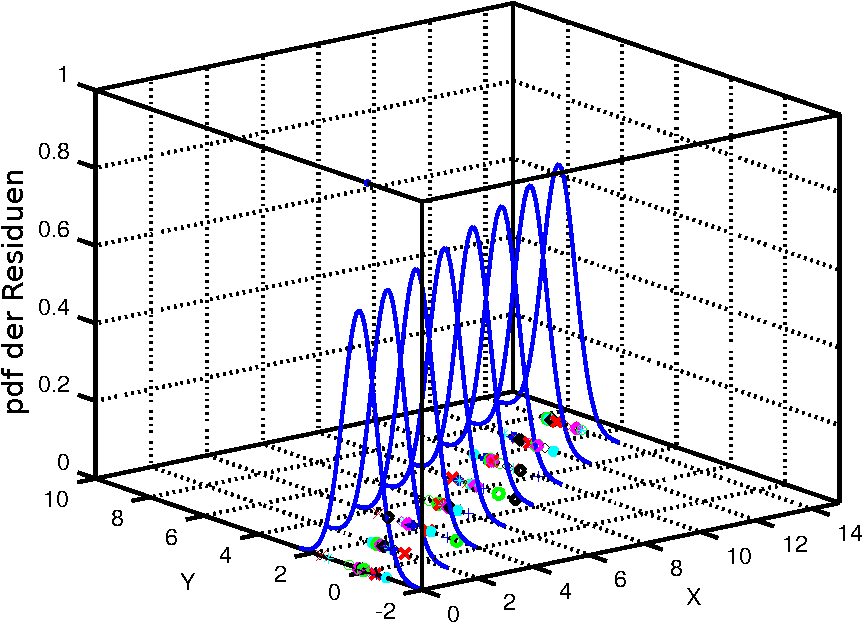
\includegraphics[width=100mm]{03_vorlesung/media/regressionNormalResi_1b.pdf}
		\caption{\label{regressionNormalResi} Lineare Regression für unabhängig und
			identisch verteilte Residuen.}
	\end{center}
\end{figure}

Abb.~\ref{regressionNormalResi} veranschaulicht, dass die Residuen normalverteilt sind, wobei die vertikale Achse die Wahrscheinlichkeitsdichte der Residuen darstellt. Der englische Begriff für Wahr\-schein\-lich\-keits\-dichte\-ver\-teil\-ung ist \textsl{probability density function}, kurz pdf. Die unterschiedlichen
Farben und Symbole sollen unterschiedliche Durchläufe gleicher Messvorgänge darstellen.

\section{Lineare Regression als Beispiel zur Methode der kleinsten Abweichungsquadrate}

Man bestimmt die Parameter der Regressionsfunktion $Y =
f(X)$ nun so, dass die Summe der Quadrate der
Abweichungen der Datenpunkte vom Modell (\textbf{Residuen}) $\varepsilon_j $ möglichst klein wird
(Methode der kleinsten Abweichungsquadrate nach C.~F.~Gau{\ss}),
d.h. das \textbf{Qualitätsmaß} $Q$ muss minimal werden:
\begin{equation}
Q: = \sum\limits_{j = 1}^J {\varepsilon_j ^2 = } \sum\limits_{j = 1}^J {(Y_j
	- f(X_j ))^2 \to } \,\,\min
\label{eq:Minimimierung-kleinster-Fehlerquadrate}
\end{equation}
Als Modellfunktion wählen wir einen Polynomansatz
\[
Y = f(X) \equiv p_m = \theta _m X ^m + \theta _{m
	- 1} X^{m - 1} + \cdots \theta _1 X + \theta _0
\]
$m$ bezeichnet den Grad des Polynoms. Die Anzahl der Regressionsparameter bezeichen wir mit $M = m+1$.

Die Minimumbedingung lautet dann:
\[
Q = Q(\theta _m ,\theta _{m - 1} ,\ldots ,\theta _1 ,\theta _0 ) =
\sum\limits_{j = 1}^J {(Y_j - p_m (X_j ))^2 \to } \,\,\min
\]

Die Konstanten $\hat{\theta_k}$, die die Funktion $Q$ minimieren, stellen
dann die beste Schätzung der Parameter $\theta _k $ dar. Die
Konstanten $\hat{\theta_k}$ ergeben sich aus der Berechnung der Nullstellen
der partiellen Ableitungen von $Q$:
\[
\left. {\frac{\partial Q}{\partial \theta _k }} \right|_{\theta_k
	=  \hat\theta_k } = 0,\,\,k = 0,1,\ldots ,m
\]
Als Lösung erhält man die gesuchte Modellgleichung mit den
Regressionsparametern (hier den Polynomkoeffizienten) $\hat\theta_k$:
\begin{equation}
Y = f(X) \equiv p_m = \hat\theta_m X ^m + \hat\theta_{m - 1} X
^{m - 1} + \cdots \hat\theta_1 X + \hat\theta_0
\end{equation}
Ein Schätzwert für die Varianz der Residuen, d.h.
$\mathrm{Var}(\varepsilon)$, ergibt sich durch die empirische Varianz:
\begin{equation}
\mathrm{Var}(\varepsilon) = s^2 = (\hat{\theta}_m ,\hat{\theta}_{m - 1} ,\ldots ,\hat{\theta}_1 
,\hat{\theta_0} ) = \frac{Q(\hat{\theta}_m ,\hat{\theta}_{m - 1}
	,\ldots ,\hat{\theta}_1 ,\hat{\theta_0} )}{J - 1 - m}
\label{eq:s_quadrat_Regresssion}
\end{equation}


Wir betrachten zunächst den einfacheren Fall der \textbf{linearen Regression},
bei dem eine empirische Regressionsgerade  gesucht wird, d.~h. 
es gibt nur zwei Modellparameter $\theta_0$ und $\theta_1$:
\begin{equation}
Y = \theta_0 + \theta_1 \cdot X
\end{equation}
Die beste Schätzung für die Parameter $\theta _0 $und
$\theta _1 $ findet man durch Minimierung gemäß
Gl.~(\ref{eq:Minimimierung-kleinster-Fehlerquadrate}),
d.~h.
\begin{equation}
\label{eq:linRegrMinimierung}
Q(\theta _0 ,\theta _1 ) = \sum\limits_{j = 1}^J {(Y_j
	- (\theta _0 + \theta _1 \cdot X_j))^2 \to } \,\,\min
\end{equation}

Für jedes vorgegebene Messwertpaar-Ensemble $(X_j ,Y_j )$, $j
= 1,2,\ldots J$ existiert eine eindeutige Lösung der Gl.
(\ref{eq:linRegrMinimierung}).

Zum Auffinden des Minimums der Gl.(\ref{eq:linRegrMinimierung}), bildet man die
partiellen Ableitungen und setzt diese gleich Null:
\[
\left. {\frac{\partial Q(\theta _0 ,\theta _1 )}{\partial \theta
		_0 }} \right|_{\theta _0 = \hat{\theta}_0 ,\,\theta _1 
	= \hat{\theta}_1 } = \left.
{\frac{\partial Q(\theta _0 ,\theta _1 )}{\partial \theta _1 }}
\right|_{\theta _0 = \hat{\theta}_0 ,\,\theta _1 = \hat{\theta}_1 } = 0
\]
\begin{center}
	mit $ \;\; \left. {\frac{\partial^2 Q(\theta _0 ,\theta _1 )}{\partial
			\theta_0^2 }} \right|_{\theta _0 = \hat{\theta}_0 ,\,\theta _1 = \hat{\theta}_1 } >
	0\;\;\;;\;\;\;\;\left. { \frac{\partial^2 Q(\theta _0 ,\theta _1
			)}{ \partial \theta_1^2 }} \right|_{\theta _0 = \hat{\theta}_0 ,\,\theta _1 =
		\hat{\theta}_1 } > 0$
\end{center}

Daraus folgt:
\[
\sum\limits_{j = 1}^J {Y_j - J} \cdot \hat{\theta}_0 - \hat{\theta}_1 \sum\limits_{j = 1}^J {X_j = 0}
\]
\[
\sum\limits_{j = 1}^J {Y_j X_j - a_0 \sum\limits_{j = 1}^N {X_j -
		a_1 \sum\limits_{j = 1}^J {X_j ^2 = 0} } }
\]

Mit $\sum\limits_{j = 1}^J {X_j } = J \cdot \bar {X}$ und $\sum\limits_{j
	= 1}^J {Y_j } = J \cdot \bar {Y}$ folgt:
\[
J \cdot \bar {Y} - J \cdot \hat{\theta}_0 - J \cdot \hat{\theta}_1 \cdot \bar {X} = 0 \quad\mathrm{bzw.}\quad \hat{\theta}_0 = \bar {Y} - \hat{\theta}_1 \cdot \bar {X}
\]

\[
\sum\limits_{j = 1}^J {X_j \cdot Y_j - \hat{\theta}_0 \cdot n \cdot \bar {X}} - \hat{\theta}_1 \sum\limits_{j = 1}^J {X_j ^2 = 0}
\]

Diese beiden Gleichungen ineinander eingesetzt, ergibt sich dann:
\[
\hat{\theta}_0 = \bar {Y} - \hat{\theta}_1 \bar {X} \quad \mathrm{und} \quad
\hat{\theta}_1 = \frac{\sum\limits_{j =
		1}^J {(X_j Y_j - \bar {X}\bar {Y})} }
{\sum\limits_{j = 1}^J {(X_j
		- \bar {X})^2} }
\]

Durch Verwendung der empirischen Varianz
\[
s_X^2 = \frac{1}{J - 1}\sum\limits_{j = 1}^J {(X_j - \bar {X})^2}
\]
\noindent und der empirischen Kovarianz:
\[
s_{XY} = \frac{1}{J - 1}\sum\limits_{j = 1}^J {(X_j - \bar
	{X})(Y_j - \bar {Y})}
\]
\noindent ergibt sich für die gesuchten Regressionsparameter
$\hat{\theta}_0$ und $\hat{\theta}_1 $:
\begin{equation}
\hat{\theta}_0 = \bar {Y} - \hat{\theta}_1 \bar {X} \quad \mathrm{und} \quad
\hat{\theta}_1 = \frac{s_{XY} }{s_X^2 }
\label{eq:Lineare_Regressionskonstanten}
\end{equation}
An dieser Gleichung sieht man, dass der Punkt $(\bar {X},\bar
{Y})$, den man auch als Schwerpunkt bezeichnet, stets auf der
Regressionsgeraden liegt. Hier wurde angenommen, dass $X$
als unabhängige und $Y $ als abhängige
Zufallsvariable betrachtet wird. Oft ist es jedoch inhaltlich
nicht klar, welche der beiden Zufallsvariablen die abh\"{a}ngige
ist. In solch einem Fall kann man zusätzlich die Regression
von $X$ auf $Y$ durchführen. Trägt man beide
Regressionsgeraden in das gleiche Koordinatensystem ein, so
schneiden sich diese stets im Schwerpunkt $(\bar {X},\bar {Y})$.

Für den Schätzwert der Varianz der
Residuen ergibt sich, siehe Gl.(\ref{eq:s_quadrat_Regresssion})

\begin{equation}
s^2(\hat{\theta}_0 ,\hat{\theta}_1 ) = \frac{Q(\hat{\theta}_0 ,
	\hat{\theta}_1 )}{J - 1 - m } 
= \frac{Q(\hat{\theta}_0 ,
	\hat{\theta}_1 )}{J - 2}
\end{equation}
 
%\begin{figure}[!htbp]
%	\centering
%	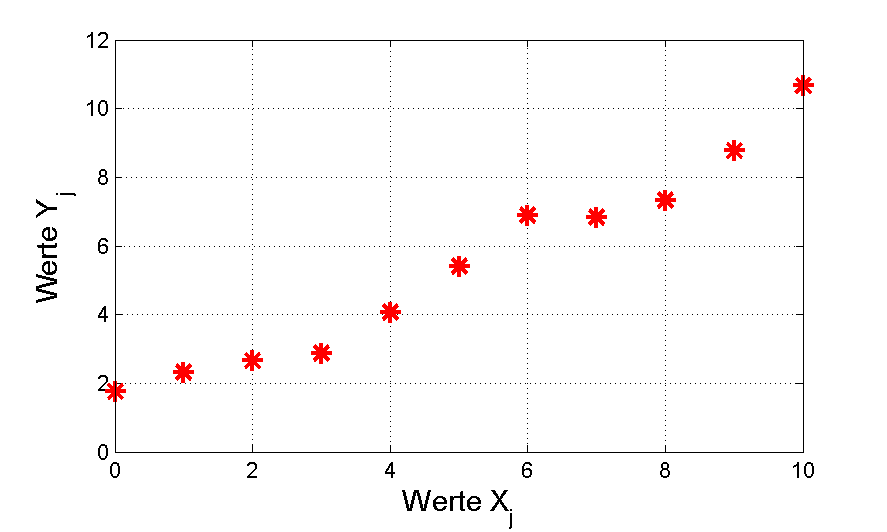
\includegraphics[width=12cm]{./Bilder/WertePaare_fuer_Regression.png}
%	\caption{Gegebene Wertepaare $X_j, Y_j$} \label{fig:Messwertpaare}
%\end{figure}

\section{Beispiele zur linearen Regression}
\label{subsection:lineare-Regression}
\textbf{Beispiel:} Vergleich der Modellierung mit Gerade und mit Polynom 6.~Grades \\
Gegeben sei ein Ensemble von Werte
$(X_j,Y_j )$, $j = 1,2,\ldots ,J$ einer Eingangsgröße (Regressor) $X$ und einer Zufallsgrößen,
der abhängigen Ausgangsgröße (Regressand) $Y$.
Beispielhaft ist in Abb.~\ref{fig:LineareRegression} eine
entsprechende Punktwolke dargestellt:
\begin{figure}[!htbp]
	\centering
	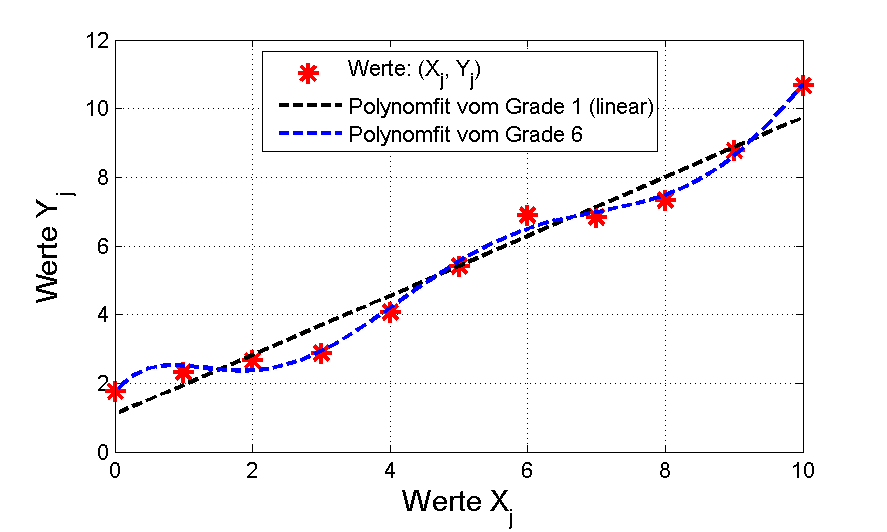
\includegraphics[width=13cm]{03_vorlesung/media/Regression_der_WertePaare.png}
    \caption{Beispiel für mögliche Fits, linearer Fit und Polynomfit vom Grade 6} \label{fig:LineareRegression}
\end{figure}
Bevor man mit der Regressionsrechnung anfängt, muss man sich im vorhinein sehr sorgfältig
überlegen, in welchem physikalischen Zusammenhang die Größen stehen, also welcher
Ansatz für das Messsystem als Modellgleichung sinnvoll ist.
In einigen Fällen ist dies auch eine Frage, welche Näherung für welchen Messbereich
ausreicht. Abb.~\ref{fig:LineareRegression} illustriert die Abweichung der Wertepaare von den unterschiedlichen Modellen und damit wie gut verschiedene Modelle die Daten approximieren.

\textbf{Beispiel:} Bestimmung des Widerstandes $R$ durch lineare Regression \\
Wir erinnern uns wieder an das Beispiel aus der 1. Vorlesung (siehe z.~B. dort Abb.~1) und bestimmen den Ohmschen Widerstand $R$ sowie eine Offsetspannung $U_0$ bei gegebenen Werten einer
Präzisions\-strom\-quelle (Regressor, genau bekannt, d.h.\ keine Zufallsgröße) und beobachteten
Werten eines Voltmeters (Regressand, Zufallsgröße). 
Der Ohmsche Widerstand $R$ und die Offsetspannung $U_0$ sind die zu bestimmenden Modellparameter (Zufallsgrößen)

\begin{center}
	\begin{tabular}{l||c|c|c|c|c|c|c|c|c}
			\hline\hline
			$I$ in mA &    4.0 &     6.0 &     8.0 &    10.0 &    12.0 &    14.0 &    16.0 &    18.0 &    20.0\\
			\hline
			$U$ in mV &    62.5 &    51.5 &    96.0 &   140.2 &   138.9 &   195.1 &   225.8 &   207.8 &   223.7 \\
			\hline\hline
	\end{tabular}
\end{center}

Die Modellgleichung lautet mit den beiden Modellparametern 
$\theta_0 :=U_0$ und $\theta_1:=R$ 
\begin{equation}
U = U_0 + R \cdot I
\end{equation}

Die beiden Modellparameter können wir mit den beiden Gleichungen (siehe Gl. (\ref{eq:Lineare_Regressionskonstanten})) bestimmt werden.
\begin{equation}
\hat{U}_0 = \bar {U} - \hat{R} \bar {I} \quad \mathrm{und} \quad
\hat{R} = \frac{s_{IU} }{s_I^2 }
\label{eq:Lineare_Regressionskonstanten_Widerstand}
\end{equation}
Zunächst bestimmen wir die beiden Mittelwerte (Einheiten lassen
wir einfachheitshalber zunächst weg):
\begin{equation}
\bar{I}\; := \; \frac{1}{J} \, \sum\limits_{j = 1}^J \, I_j
= 12 
\qquad 
\bar{U} \; := \; \frac{1}{J} \, \sum\limits_{j = 1}^J \, U_j
= 149.0556
\end{equation}
Die empirische Kovarianz mit den $J = 9$ Stichproben ergibt sich zu: 
\[
s_{IU} = \frac{1}{J - 1}\sum\limits_{j = 1}^J {(I_j - \bar
	{R})(U_j - \bar {U})} = 357.0500
\]

Die Varianz ergibt sich zu: 
\[
s_I^2 = \frac{1}{J - 1}\sum\limits_{j = 1}^J {(I_j - \bar {I})^2} = 30
\]

Somit erhalten wir als Schätzwert für $R$
\[
\hat{R} = \frac{s_{IU} }{s_I^2} = 357.050/30 = 11.9017
\]
und als Schätzwert für $U_0$: 
\[
\hat{U}_0 = \bar {U} - \hat{R} \bar {I} = 149.0556 -  11.9017 \cdot 12 =
6.2356
\]

Das Ergebnis für die Regressionsgerade lautet somit und ist in Abb.~\ref*{fig:LineareRegressionWiderstand} visualisiert.
\begin{equation}
U = 6.2356 + 11.9017 \cdot I 
\end{equation}
\begin{figure}[!htbp]
	\centering
	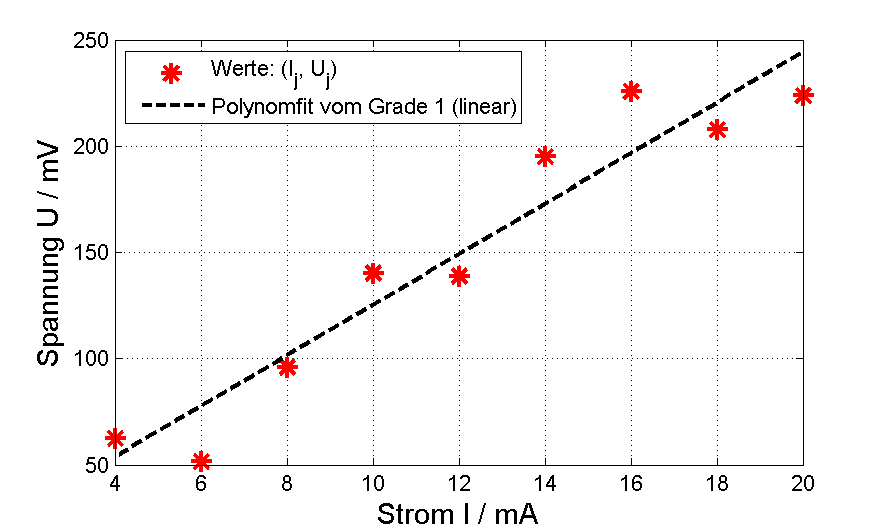
\includegraphics[width=13cm]{03_vorlesung/media/Regression_der_WertePaare_Strom_Spannung.png}
	\caption{Beispiel: Bestimmung des Ohmschen Widerstand und einer Offset-Spannung durch lineare Regression} \label{fig:LineareRegressionWiderstand}
\end{figure}
% \end{quote}	

\section{Varianz der Regressionsparameter}
\label{subsec:vertrauensbereiche}

Es können aus den Messreihen die Varianzen der
geschätzten Regressionsparameter ermittelt werden. Das Verfahren zeigen wir
hier anhand der Regressionsgeraden mit den geschätzten Parametern
Achsenabschnitt $\hat{\theta}_0 $ und Steigung $\hat\theta_1 $.
Damit hat man ein Ma{\ss} f\"{u}r die statistische
Sicherheit der Sch\"{a}tzung der Parameter $\theta _0 $ und
$\theta _1 $.
Für die Varianz des Regressionsparameters $\hat{\theta}_1 $
gilt:
\begin{equation}
\sigma^2_{\hat{\theta}_1} = \frac{ \hat \sigma^2_{\varepsilon}}{s^2_X \cdot (J- 1) }
\end{equation}

Für die Varianz des Regressionsparameters $\hat{\theta}_0 $
gilt:
\begin{equation}
\sigma^2_{\hat{\theta}_0} = \hat \sigma^2_{\varepsilon} \cdot \left(\frac{1}{J}
	+ \frac{\bar {X}^2}{(J - 1) s_X^2 }\right)^2
\end{equation}
\begin{center}
\end{center}

Die Varianz des Achsenabschnittes wird weiter unten in der Gl.(\ref{eq:Varianz des Achsenabschnitts}) hergeleitet. Dort ergibt sich (Hinweis: Wir haben dort den Achsenabschnitt mit $\theta_0$ bezeichnet und nicht wie hier mit $\theta_1$ ) 
\begin{equation}
\hat \sigma^2_{\theta_0}  = \hat \sigma^2_{\varepsilon}  \sum(X_j^2)  / (J \sum(X_j^2) - (\sum(X_j))^2) 
\end{equation}
Wir bezeichnen nun das $\hat \sigma^2_{\varepsilon}$ hier mit $s^2_{\varepsilon}$ und erhalten:
\begin{equation}
\hat \sigma^2_{\theta_0}  = s^2_{\varepsilon} \sum(X_j^2)  / (J \sum(X_j^2) - (\sum(X_j))^2) 
\end{equation}
\begin{equation}
\hat \sigma^2_{\theta_0} = s^2_{\varepsilon} \frac{1}{J} \sum(X_j^2)  / (\sum(X_j^2) - \frac{1}{J}(\sum(X_j))^2)
\end{equation}
Mit der folgenden Null-Identität
\begin{equation}
0 =  - \frac{1}{J}(\sum(X_j))^2 + \frac{1}{J}(\sum(X_j))^2
\end{equation}
gilt
\[
(1/J) \sum(X_j^2)  / (\sum(X_j^2) - \frac{1}{J}(\sum(X_j))^2) = 
\]
\[
(1/J) [\sum(X_j^2) - (1/J)(\sum(X_j))^2 + \frac{1}{J}(\sum(X_j))^2] / (\sum(X_j^2) - (1/J)(\sum(X_j))^2)
\]
das heisst
\[
\frac{1}{J} \sum(X_j^2)  / (\sum(X_j^2) - \frac{1}{J}(\sum(X_j))^2) =
\]
\[
(1/J) [ 1 + \frac{1}{J}(\sum(X_j))^2 / (\sum(X_j^2) - \frac{1}{J}(\sum(X_j))^2) ]
\]

und mit $(\sum(X_j^2) - \frac{1}{J}(\sum(X_j))^2) = (J-1) s_X^2$ gilt dann
\begin{align}
\hat \sigma^2_{\theta_0} =& 
s^2_{\varepsilon} \frac{1}{J} \sum(X_j^2)  / (\sum(X_j^2) - \frac{1}{J}(\sum(X_j))^2) \\
=& s^2_{\varepsilon} \frac{1}{J} \sum(X_j^2)  / (J-1) s_X^2
\end{align}
und mit der Umformung der Null-Identität gilt dann
\begin{align}
\hat \sigma^2_{\theta_0} 
=& s^2_{\varepsilon} \frac{1}{J} \sum(X_j^2)  / (\sum(X_j^2) - \frac{1}{J}(\sum(X_j))^2) \\
=& s^2_{\varepsilon} \frac{1}{J} \left[ 1 + \frac{1}{J}(\sum(X_j))^2 / (\sum(X_j^2) - \frac{1}{J}(\sum(X_j))^2) \right] \\
=& s^2_{\varepsilon} \frac{1}{J} \left[ 1 + \frac{1}{J(J-1) s_X^2} \left(\sum(X_j)\right)^2 \right]  
\end{align}
mit $\frac{1}{J}(\sum(X_j)) = \bar X$ gilt $\frac{1}{J}(\sum(X_j))^2 = J \bar X^2$
so dass
\begin{align}
\hat \sigma^2_{\theta_0} =& s_{\varepsilon} \frac{1}{J} \left[ 1 + 
\frac{1}{J (J-1) s_X^2} \left(\sum(X_j) \right)^2 \right] \\
=& s^2_{\varepsilon} \frac{1}{J(J-1) s_X^2} \left[ 1 + (J \bar X^2) \right] \\
=&
s^2_{\varepsilon}  \left[\frac{1}{J} + \frac{\bar X^2}{(J-1) s_X^2} \right]
\end{align}

Damit erhalten wir für die \textbf{Varianz bzw. die Unsicherheit des Achsenabschnittes}: 
\begin{equation}
\hat \sigma^2_{\theta_0} =
s^2_{\varepsilon}  \left[ \frac{1}{J} +\frac{\bar {X}^2}{(J - 1) s_X^2 } \right]
\end{equation}

\section{Regression mit mehr als zwei Modellparametern}
Die beiden Modellparameter der linearen Regression benennen wir hier um und heißen hier $\theta_1$ für den Achsenabschnitt (vorher $\theta_0$ ) und $\theta_2$ für die Geradensteigung (bisher $\theta_1$).
Als Regressormatrix verwenden wir jetzt
\begin{equation}
\mathbf{X} \; = \;
\left(
\begin{array}{cc}
1 &  X_{1,1} \\
\vdots & \vdots\\
1 & X_{1,J} 
\end{array}
\right)
\end{equation}
Die Residuen berechnen sich wie folgt: 
\begin{equation}
\left(
\begin{array}{c}
\varepsilon_1\\
\vdots \\
\varepsilon_J
\end{array}
\right)  \; = \;
\left(
\begin{array}{c}
Y_{1} \; - \; (1 \, \theta_1 \; + \;  X_{1,1} \, \theta_2)\\
\vdots \\
Y_{J} \; - \; (1 \, \theta_1 \; + \;  X_{1,J} \, \theta_2)
\end{array}
\right) \; = \;
\left(
\begin{array}{c}
Y_{1}\\
\vdots \\
Y_{J}
\end{array}
\right) 
\; - \; 
\left(
\begin{array}{cc}
1 &  X_{1,1} \\
\vdots & \vdots\\
1 & X_{1,J} 
\end{array}
\right) 
\left(
\begin{array}{c}
\theta_1\\
\theta_2
\end{array}
\right)
\label{linearRegressionGeradeTheta}
\end{equation}
Die Summe der Quadrate der Residuen $\sum_{j=1}^J \varepsilon_j^2$ lässt sich ebenso
mit der Rechenregel Zeile mal Spalte schreiben, als Zeilenvektor mal Spaltenvektor
\begin{equation}
\sum_{j=1}^J \varepsilon_j^2 \; = \; 
\left(\begin{array}{ccc}
\varepsilon_1 & \dots & \varepsilon_J
\end{array}
\right)
\left(
\begin{array}{c}
\varepsilon_1\\
\vdots \\
\varepsilon_J
\end{array}
\right)
\end{equation}
Dabei heißt der Zeilenvektor der transponierte Vektor, also
\begin{equation}
\boldsymbol{\varepsilon}^\mathsf{T} \; = \; \left(\begin{array}{ccc}
\varepsilon_1 & \dots & \varepsilon_J
\end{array}
\right) \qquad \mathrm{und}  \qquad 
\boldsymbol{\varepsilon} \; = \; \left(
\begin{array}{c}
\varepsilon_1\\
\vdots \\
\varepsilon_J
\end{array}
\right)
\end{equation}
und ferner führen wir ein
\begin{equation}
\boldsymbol{\theta} \; = \;
\left(
\begin{array}{c}
\theta_1\\
\theta_2
\end{array}
\right) \qquad \mathrm{und}  \qquad 
\mathbf{Y}  \; = \;\left(
\begin{array}{c}
Y_{1}\\
\vdots \\
Y_{J}
\end{array}
\right) 
\end{equation}
und Gl.~(\ref{linearRegressionGeradeTheta}) sieht in transponierter Schreibweise
wie folgt aus
\begin{equation}
\boldsymbol{\varepsilon}^\mathsf{T} \; = \;
\mathbf{Y}^\mathsf{T}
\; - \; 
\boldsymbol{\theta}^\mathsf{T} \left(
\begin{array}{cc}
1 &  X_{1,1} \\
\vdots & \vdots\\
1 & X_{1,J} 
\end{array}
\right)^\mathsf{T} 
\label{linearRegressionGeradeTransponiert}
\end{equation}
d.h.
\begin{equation}
\boldsymbol{\varepsilon}^\mathsf{T} \; = \;
\mathbf{Y}^\mathsf{T}
\; - \; 
\left(
\begin{array}{cc}
\theta_1 &
\theta_2
\end{array}
\right) \left(
\begin{array}{ccc}
1 &  \dots & 1 \\
X_{1,1} & \dots & X_{1,J} 
\end{array}
\right).
\label{linearRegressionGeradeUmform}
\end{equation}
Die Summe der Quadrate der Residuen $\sum_{j=1}^J \varepsilon_j^2$  sieht damit wie
folgt aus
\begin{equation}
\boldsymbol{\varepsilon}^\mathsf{T}  \boldsymbol{\varepsilon} \; = \;
\left(
\mathbf{Y}^\mathsf{T}
\; - \; 
\boldsymbol{\theta}^\mathsf{T} \mathbf{X}^\mathsf{T} \right)
\left(
\mathbf{Y}
\; - \; 
\mathbf{X} \boldsymbol{\theta} \right)
\end{equation}
d.h.
\begin{equation}
\boldsymbol{\varepsilon}^\mathsf{T}  \boldsymbol{\varepsilon} \; = \;
\mathbf{Y}^\mathsf{T} \mathbf{Y}
\; - \; 
\boldsymbol{\theta}^\mathsf{T} \mathbf{X}^\mathsf{T}  \mathbf{Y} 
\; - \; 
\mathbf{Y}^\mathsf{T}  \mathbf{X} \boldsymbol{\theta}
\; + \; 
\boldsymbol{\theta}^\mathsf{T} \mathbf{X}^\mathsf{T} \mathbf{X} \boldsymbol{\theta}
\end{equation}
Für die Ableitungen nach den $\theta_1, \theta_2$ gilt
\begin{equation}
\frac{\partial}{\partial \theta_l} \sum_{j=1}^J \varepsilon_j^2 \; = \; 
2 \sum_{j=1}^J \varepsilon_j \frac{\partial}{\partial \theta_l} \varepsilon_j \; = \; 
2 \sum_{j=1}^J \varepsilon_j (-1) \frac{\partial}{\partial \theta_l}(1 \, \theta_1 \; + \;  X_{1,j} \, \theta_2) \; = \; 0
\end{equation}
wobei $l = 1,2$ ist also
\begin{equation}
\sum_{j=1}^J \varepsilon_j  \frac{\partial}{\partial \theta_1}(1 \, \theta_1 \; + \;  X_{1,j} \, \theta_2)  \; = \; 0 \qquad \mathrm{und} \qquad 
\sum_{j=1}^J \varepsilon_j  \frac{\partial}{\partial \theta_2}(1 \, \theta_1 \; + \;  X_{1,j} \, \theta_2)  \; = \; 0
\end{equation}
also
\begin{equation}
\sum_{j=1}^J \varepsilon_j (1) \; = \; 0 \qquad \mathrm{und}  \qquad 
\sum_{j=1}^J \varepsilon_j ( X_{1,j})  \; = \; 0
\end{equation}
Dies sieht in Matrixschreibweise als $2 \times 2$-Gleichungssystem wie folgt aus
\begin{equation}
\boldsymbol{\varepsilon}^\mathsf{T} \, \mathbf{X} \; = \;
\left(
\begin{array}{c}
0\\
0
\end{array}
\right)
\end{equation}
d.h.
\begin{equation}
\left(\mathbf{Y}^\mathsf{T}
\; - \; 
\boldsymbol{\theta}^\mathsf{T} \mathbf{X}^\mathsf{T} \right) \, \mathbf{X} \; = \;
\left(
\begin{array}{c}
0\\
0
\end{array}
\right)
\end{equation}
d.h.
\begin{equation}
\boldsymbol{\theta}^\mathsf{T} \, \mathbf{X}^\mathsf{T}  \, \mathbf{X} \; = \;
\mathbf{Y}^\mathsf{T} \, \mathbf{X}
\end{equation}
%$\frac{\partial}{\partial \beta_l} \varepsilon_j$ auf.
%Der Vektor mit für die partielle Differentiation heißt Nablaoperator
%\begin{equation}
%\nabla_\beta \; = \;
%\left(
%\begin{array}{cc}
%\frac{\partial}{\partial \beta_0} &
%\frac{\partial}{\partial \beta_1}
%\end{array}
%\right)
%\end{equation}
das ist äquivalent zu
\begin{equation}
\mathbf{X}^\mathsf{T} \, \mathbf{X} \, \boldsymbol{\theta} \; = \;
\mathbf{X}^\mathsf{T} \, \mathbf{Y} .
\end{equation}
Die numerische Lösung des Gleichungssystems liefert dann die Schätzwerte zu
den Regressionparametern $\boldsymbol{\theta}$. Ein mögliches Verfahren zum
Lösen des linearen Gleichungssystems ist das Gauß-Jordan-Eliminationsverfahren, zu
dem im Anhang dieses Skripts der Quellcode gemäß den \textsl{Numerical Recipes}
\cite{Fla02} abgedruckt ist.
Formal notieren wir 
die Schätzer (als solche kenntlich durch das Dach) wie folgt
\begin{equation}
\boldsymbol{\hat \theta} \; = \;
\left( \mathbf{X}^\mathsf{T}  \, \mathbf{X} \right)^{-1} \mathbf{X}^\mathsf{T} \, \mathbf{Y}
\end{equation}
wobei hoch minus Eins soviel bedeutet wie die Inverse der Matrix.

Als nächstes ermitteln wir, um das \textbf{vollständige
	Messergebnis} zu erhalten, auch die Schätz\-werte der Kovarianzen. Die
Hauptdiagonale der Kovarianzmatrix sind die Varianzen.
\begin{equation}
\operatorname {Cov}( \boldsymbol{\theta},\boldsymbol{\theta} ) \; = \;
\operatorname {Cov} 
\left(\left( \mathbf{X}^\mathsf{T}  \, \mathbf{X} \right)^{-1} \mathbf{X}^\mathsf{T} \, \mathbf{Y}, \left( \mathbf{X}^\mathsf{T}  \, \mathbf{X} \right)^{-1} \mathbf{X}^\mathsf{T} \, \mathbf{Y}\right)
\end{equation}
%mit Gl.~(\ref{CovarianzKonstMatrix}) ist dies
das ist
\begin{equation}
\operatorname {Cov}( \boldsymbol{\theta}, \boldsymbol{\theta} ) \; = \;
\left( \mathbf{X}^\mathsf{T}  \, \mathbf{X} \right)^{-1} \mathbf{X}^\mathsf{T} \operatorname {Cov} (\mathbf{Y}, \mathbf{Y}) \, \left( \left( \mathbf{X}^\mathsf{T}  \, \mathbf{X} \right)^{-1} \mathbf{X}^\mathsf{T} \right)^\mathsf{T}
\end{equation}
und mit Einsetzen der aus den Schätzern $\boldsymbol{\hat \theta}$ erhaltenen
empirischen Varianz der Residuen 
$\operatorname {Cov} (\mathbf{Y}, \mathbf{Y}) = \operatorname {Var} (\mathbf{\varepsilon}) = \hat \sigma_{\varepsilon}^2$
bekommen wir die empirische Kovarianzmatrix
\begin{equation}
\boldsymbol{\hat \Sigma}_{\boldsymbol{\theta}} \; = \;
\hat \sigma_{\varepsilon}^2
\left( \mathbf{X}^\mathsf{T}  \, \mathbf{X} \right)^{-1} \mathbf{X}^\mathsf{T} \, \left( \left( \mathbf{X}^\mathsf{T}  \, \mathbf{X} \right)^{-1} \mathbf{X}^\mathsf{T} \right)^\mathsf{T}
\end{equation}
mit
$$
\operatorname {Var} (\mathbf{\varepsilon}) = \hat \sigma_{\varepsilon}^2 \; = \;
\frac{1}{J-M} \, \boldsymbol{\hat \varepsilon}^\mathsf{T} \boldsymbol{\hat \varepsilon}
$$
wobei $M$ die Anzahl der Regressionsparameter ist, also $M = 2$ im Fall der Geraden, für die beiden Parameter Achsenabschnitt und Steigung und
$$
\boldsymbol{\hat \varepsilon} \; = \; \mathbf{Y} \, - \, \mathbf{X} \boldsymbol{\hat \theta} .
$$

Ferner gilt mit $\left( \left( \mathbf{X}^\mathsf{T}  \, \mathbf{X} \right)^{-1} \mathbf{X}^\mathsf{T} \right)^\mathsf{T} = \mathbf{X} \left( \mathbf{X}^\mathsf{T}  \, \mathbf{X} \right)^{-1}$
\begin{equation}
\boldsymbol{\hat \Sigma}_{\boldsymbol{\theta}} \; = \; \hat \sigma_{\varepsilon}^2
\left( \mathbf{X}^\mathsf{T}  \, \mathbf{X} \right)^{-1} \mathbf{X}^\mathsf{T}  \,  \mathbf{X} \, \left( \mathbf{X}^\mathsf{T}  \, \mathbf{X} \right)^{-1} 
\end{equation}
und mit $\left( \mathbf{X}^\mathsf{T}  \, \mathbf{X} \right)^{-1} \mathbf{X}^\mathsf{T}  \, \mathbf{X}  \; = \; 1 \! \mathrm{I}$ Einheitsmatrix
\begin{equation}
\boldsymbol{\hat \Sigma}_{\boldsymbol{\theta}} \; = \; \hat \sigma_{\varepsilon}^2
\left( \mathbf{X}^\mathsf{T}  \, \mathbf{X} \right)^{-1}
\label{UnsicherheitRegressparams}
\end{equation}
Gleichung (\ref{UnsicherheitRegressparams}) liefert die Unsicherheit für die Regressionsparameter
$\boldsymbol{\theta}$. 
%Sie unterscheidet sich
%Gleichung (\ref{KovarianzSumme})
Setzen wir dies nun für die Regressionsgerade ein, also setzen wir
$$
\mathbf{X} \; = \;
\left(
\begin{array}{cc}
1 &  X_{1,1} \\
\vdots & \vdots\\
1 & X_{1,J} 
\end{array}
\right)
$$
ein, so erhalten wir für
\begin{equation}
\left( \mathbf{X}^\mathsf{T}  \, \mathbf{X} \right)^{-1} \; = \;
\left( \left(
\begin{array}{ccc}
1 & \cdots & 1 \\
X_{1,1} & \cdots & X_{1,J} 
\end{array}
\right)
\, 
\left(
\begin{array}{cc}
1 &  X_{1,1} \\
\vdots & \vdots\\
1 & X_{1,J} 
\end{array}
\right) \right)^{-1}
\end{equation}
d.h.
\begin{equation}
\left( \mathbf{X}^\mathsf{T}  \, \mathbf{X} \right)^{-1} \; = \;
\left(
\begin{array}{ccc}
J & \sum\limits_{j=1}^J X_{1,j} \\
\sum\limits_{j=1}^J X_{1,j} & \sum\limits_{j=1}^J X_{1,j}^2
\end{array}
\right)^{-1}
\end{equation}
d.h.
\begin{equation}
\left( \mathbf{X}^\mathsf{T}  \, \mathbf{X} \right)^{-1} \; = \;
\frac{1}{J \, \sum\limits_{j=1}^J X_{1,j}^2 \; - \;
	\left(\sum\limits_{j=1}^J X_{1,j}\right)^2}
\left(
\begin{array}{ccc}
\sum\limits_{j=1}^J X_{1,j}^2 & -\sum\limits_{j=1}^J X_{1,j} \\
-\sum\limits_{j=1}^J X_{1,j} & J
\end{array}
\right)
\end{equation}
so dass wir für den Achsenabschnitt $\theta_1$ und die Steigung $\theta_2$ folgende
empirische Varianzen und Kovarianzen erhalten
\begin{equation}
\left(\begin{array}{cc}
\hat \sigma^2_{\theta_1} &\hat \sigma_{\theta_1, \theta_2}\\
\hat \sigma_{\theta_1, \theta_2} & \hat \sigma^2_{\theta_2} 
\end{array}\right)
\; = \;
\frac{\hat \sigma^2_\varepsilon}{J \, \sum\limits_{j=1}^J X_{1,j}^2 \; - \; 
	\left(\sum\limits_{j=1}^J X_{1,j}\right)^2}
\left(
\begin{array}{ccc}
\sum\limits_{j=1}^J X_{1,j}^2 & -\sum\limits_{j=1}^J X_{1,j} \\
-\sum\limits_{j=1}^J X_{1,j} & J
\end{array}
\right)
\end{equation}
oder einzeln aufgeschrieben, die Varianz des Achsenabschnitts
%\begin{figure}
%	\begin{center}
%		\includegraphics[width=100mm]{Bilder/regressionNormalResi_Perr_1a.eps}
%		\caption{\label{regressionParamErr} Unsicherheit der Schätzer
%			der linearen Regression einer Geradengleichung für ein
%			Vertrauensniveau von $98 \%$. Mit $\nu = J-2 = 26-2 = 24$ Freiheitsgraden
%			ist das Quantil der Student-t-Verteilung $t_{1-\alpha/2,\nu} = 2.492$.}
%	\end{center}
%\end{figure}
\begin{equation}
\hat \sigma^2_{\theta_1} \; = \; 
\frac{\hat \sigma^2_\varepsilon \, \sum\limits_{j=1}^J X_{1,j}^2}{J \, 
	\sum\limits_{j=1}^J X_{1,j}^2 \; - \; \left(\sum\limits_{j=1}^J X_{1,j}\right)^2}
\label{eq:Varianz des Achsenabschnitts}
\end{equation}
die Kovarianz für Achsenabschnitt und Steigung
\begin{equation}
\hat \sigma_{\theta_1, \theta_2} \; = \; 
\frac{- \hat \sigma^2_\varepsilon \, \sum\limits_{j=1}^J X_{1,j}}{J \, \sum_{j=1}^J X_{1,j}^2 \;
	- \; \left(\sum\limits_{j=1}^J X_{1,j}\right)^2}
\end{equation}
und die Varianz der Steigung
\begin{equation}
\hat \sigma^2_{\theta_2} \; = \; 
\frac{\hat \sigma^2_\varepsilon}{\sum\limits_{j=1}^J X_{1,j}^2 \; - \; 
	\frac{1}{J}\left(\sum\limits_{j=1}^J X_{1,j}\right)^2} .
\end{equation}
Die Standardabweichungen zu jedem Regressionsparameter $\theta_l$ mit $l = 1,\dots,M$ sind
die Wurzel aus den Varianzen, die auf der Hauptdiagonalen der Kovarianzmatrix 
$\left( \mathbf{X}^\mathsf{T}  \, \mathbf{X} \right)^{-1} \, \hat \sigma_{\varepsilon}^2$
stehen. In der üblichen englischsprachigen Literatur zur Regressionrechnung wird
die Standardabweichung der Regressionsparameter \textsl{Standard Error} genannt.

Wir definieren folgende $M$-dimensionale Einheitsvektoren
\begin{equation}
\boldsymbol{e}_l \; = \;
\left(\begin{array}{c}
0\\
\vdots\\
0\\
1\\
0\\
\vdots\\
0
\end{array}\right)
\end{equation}
bei dem die ersten $l-1$ Vektorkomponenten Nullen sind, an der $l$-ten Stelle eine Eins steht
und die $l+1$-te Komponente bis zur $M$-ten wieder Nullen sind.
Dann lässt sich durch folgende Multiplikation die $l$-te Varianz, d.h. das $l$-te Element
der Hautpdiagonalen aus der Kovarianzmatrix herausholen
\begin{equation}
\hat \sigma_l^2 \; = \; \boldsymbol{e}_l^\mathsf{T} \, \left( \mathbf{X}^\mathsf{T}  \, \mathbf{X} \right)^{-1} \, \boldsymbol{e}_l  \; \hat \sigma_{\varepsilon}^2 .
\end{equation}
Die Standardabweichung (\textsl{Standard Error}) wird daraus durch Ziehen der Wurzel
gewonnen
\begin{equation}
\hat \sigma_l \; = \; \sqrt{\hat \sigma_l^2} .
\end{equation}
In einer der nächsten Vorlesungen werden wir dann sehen, wie man mit Hilfe der Varianzen bzw. Standardabweichungen Vertrauensintervalle für die geschätzten Modellparameter bestimmt.

%Das vollständige Messergebnis für jeden der Regressionparameter ist damit
%\begin{equation}
%\theta_l \; = \;
%\boldsymbol{e}_l^\mathsf{T} \, \left( \mathbf{X}^\mathsf{T}  \, \mathbf{X} \right)^{-1} %\mathbf{X}^\mathsf{T} \, \mathbf{Y}
%\; \pm \; t_{1-\alpha/2, \nu} \, \hat \sigma_l
%\end{equation}
%mit $\nu = J-M$ und die Korrelationskoeffizienten für die Korrelation der %Regressionsparameter
%untereinander sind
%\begin{equation}
%\rho_{l,m} \; = \; \frac{\hat \sigma_{\varepsilon}^2}{\hat \sigma_l \, \hat \sigma_m} \; %\boldsymbol{e}_l^\mathsf{T} \, \left( \mathbf{X}^\mathsf{T}  \, \mathbf{X} \right)^{-1} %\, \boldsymbol{e}_m  .
%\end{equation}

\section{Allgemeiner Ansatz der linearen Regression}

Die behandelten allgemeinen Formen von Problemstellungen zur Schätzung von Modellparametern
werden wir in dieser Vorlesungsreihe nicht weiter vertiefen. Sie sollen lediglich einen Einblick
und Überblick über die vielfältigen Möglichkeiten in diesem Bereich liefern.
In den Übungen und der Klausur werden
wir uns auf das Schätzverfahren mittels linearer Regression fokussieren.


Um die lineare Regression universeller einsetzen zu können, ob nun Polynome oder
Ebenen oder Paraboloide zu fitten sind, ist es erforderlich den allgemeinen Ansatz zu verstehen
und die unterschiedlichen Anwendungen so formulieren zu können, dass sie darüber lösbar werden.

Vor einer Woche wurde der allgemeine Ansatz anhand
einer Regressionsgeraden hergleitet
\begin{equation}
\left(
\begin{array}{c}
\varepsilon_1\\
\vdots \\
\varepsilon_J
\end{array}
\right)  \; = \;
\left(
\begin{array}{c}
 Y_{1} \; - \; (1 \, \theta_0 \; + \;  X_{1,1} \, \theta_1)\\
\vdots \\
 Y_{J} \; - \; (1 \, \theta_0 \; + \;  X_{1,J} \, \theta_1)
\end{array}
\right) \; = \;
\left(
\begin{array}{c}
 Y_{1}\\
\vdots \\
 Y_{J}
\end{array}
\right) 
\; - \; 
\left(
\begin{array}{cc}
 1 &  X_{1,1} \\
\vdots & \vdots\\
 1 & X_{1,J} 
\end{array}
\right) 
\left(
\begin{array}{c}
\theta_0\\
\theta_1
\end{array}
\right)
\label{linearRegressionGeradeTheta}
\end{equation}
wobei die Matrix auf der rechten Seite mit dem Begriff \textsl{Regressormatrix} eingeführt wurde:
\begin{equation}
\mathbf{X} \; = \;
\left(
\begin{array}{cc}
 1 &  X_{1,1} \\
\vdots & \vdots\\
 1 & X_{1,J} 
\end{array}
\right)
\end{equation}
Für $M$ Regressoren wird die Regressormatrix zu einer $J \times M$-Matrix, also einer Matrix
aus $M$ Spalten und $J$ Zeilen:
\begin{equation}
\mathbf{X} \; = \;
\left(
\begin{array}{ccc}
 X_{1,1} & \dots &  X_{M,1} \\
\vdots & & \vdots \\
 X_{1,J}  & \dots &  X_{M,J}
\end{array}
\right)
\end{equation}
Die Indexschreibweise ist hier relativ zur Schreibweise der Matrizenrechnung vertauscht, weil wir den Index für die
Messgrößen vorne haben gefolgt von dem Index für die Beobachtungen, wir aber die Messgrößen als
Spaltenvektoren verwenden und somit den Index für die Beobachtungen als Zeilenindex haben.

\begin{equation}
\boldsymbol{\varepsilon} \, =  \, \left(
\begin{array}{c}
\varepsilon_1\\
\vdots \\
\varepsilon_J
\end{array}
\right)  \; = \;
\left(
\begin{array}{c}
 Y_{1} \; - \; (X_{1,1} \, \theta_1  \; + \; \dots  \; + \;  X_{M,1} \, \theta_{M})\\
\vdots \\
 Y_{J} \; - \; (X_{1,J} \, \theta_1 \; + \; \dots  \; + \;  X_{M,J} \, \theta_{M})
\end{array}\right)  \, = \, 
\mathbf{Y} \, -  \, \mathbf{X} \, \boldsymbol{\theta}
\end{equation}
Im Fall eines Polynoms kann jeder der Regressoren Funktion derselben Messgröße sein.
Dies kann beispielsweise einfach
durch folgenden Potenzansatz $X_{m,j} = X_{1,j}^{m-1}$ mit $m = 1,\dots,M$ als
Polynom vom Grad $M-1$ dargestellt werden
\begin{equation}
\left(
\begin{array}{c}
\varepsilon_1\\
\vdots \\
\varepsilon_J
\end{array}
\right)  \; = \;
\left(
\begin{array}{c}
 Y_{1} \; - \; (X_{1,1}^0 \, \theta_1  \; + \; \dots  \; + \;  X_{1,1}^{M-1} \, \theta_{M})\\
\vdots \\
 Y_{J} \; - \; (X_{1,J}^0 \, \theta_1 \; + \; \dots  \; + \;  X_{1,J}^{M-1} \, \theta_{M})
\end{array}\right)
\end{equation}
wobei $X_{1,j}^0 = 1$ ist.

Wird die Regressormatrix zu Beginn korrekt aufgestellt, so lassen sich die 
$M$ Regressionsparameter $\boldsymbol{\theta}$
schätzen durch numerische Lösung des folgenden Gleichungssystems:
\begin{equation}
\mathbf{X}^\mathsf{T} \, \mathbf{X} \, \boldsymbol{\theta} \; = \;
\mathbf{X}^\mathsf{T} \, \mathbf{Y} .
\label{LsgRegressionGlSys}
\end{equation}
Dass nach Lösen des Gleichungssystems Schätzwerte für
die Parameter gewonnen wurden, wird durch das Dach auf dem Symbol $\boldsymbol{\theta}$ gekennzeichnet.
\begin{equation}
 \boldsymbol{\hat \theta} \; = \;
\left( \mathbf{X}^\mathsf{T}  \, \mathbf{X} \right)^{-1} \mathbf{X}^\mathsf{T} \, \mathbf{Y}
\end{equation}
wobei hoch minus Eins soviel bedeutet wie die Inverse der Matrix.
Für Varianzen und Kovarianzen der $M$ Regressionsparameter $\theta_1, \dots, \theta_M$
werden die Residuen gebraucht
\begin{equation}
\boldsymbol{\hat \varepsilon} \, =  \, \left(
\begin{array}{c}
\hat \varepsilon_1\\
\vdots \\
\hat \varepsilon_J
\end{array}
\right)  \; = \;
\left(
\begin{array}{c}
 Y_{1} \; - \; (X_{1,1} \, \hat \theta_1  \; + \; \dots  \; + \;  X_{M,1} \, \hat \theta_{M})\\
\vdots \\
 Y_{J} \; - \; (X_{1,J} \, \hat \theta_1 \; + \; \dots  \; + \;  X_{M,J} \, \hat \theta_{M})
\end{array}
\right) \, = \, 
\mathbf{Y} \, -  \, \mathbf{X} \, \boldsymbol{\hat \theta}
\end{equation}
um deren empirische Varianz zu berechnen
\begin{equation}
\hat \sigma_{\varepsilon}^2 \; = \;
\frac{1}{J-M} \, \boldsymbol{\hat \varepsilon}^\mathsf{T} \boldsymbol{\hat \varepsilon}
\end{equation}
so dass wir die empirische Kovarianzmatrix der Parameter erhalten:
\begin{equation}
\boldsymbol{\hat \Sigma}_{\boldsymbol{\theta}} \; = \; 
\left( \mathbf{X}^\mathsf{T}  \, \mathbf{X} \right)^{-1} \;
\hat \sigma_{\varepsilon}^2
\label{UnsicherheitRegressparams}
\end{equation}


\section{Das Bestimmtheitsmaß, empirischer Korrelationskoeffizient}
Die G\"{u}te des gew\"{a}hlten linearen Ansatzes kann mit dem
\textbf{Bestimmtheitsmaß} $\rho_{XY}^2 $ bzw. dem \textbf{empirischen
Korrelationskoeffizienten} $\rho_{XY}$ beurteilt werden, aber nur dann
wenn ein solcher Zusammenhang auch existiert. Der empirische
Korrelationskoeffizienten gibt den Grad der linearen
Abh\"{a}ngigkeit zwischen den Messwerten $(X_1 ,\ldots ,X_J )$ und
$(Y_1 ,\ldots ,Y_J)$ an. 

Für den empirischen Korrelationskoeffizienten $\rho_{XY}$ gilt folgendes:

\begin{center}
	\begin{tabular}
		{|p{100pt}|p{209pt}|} \hline 
		$\rho_{XY} = \pm 1$&
		100{\%} lineare Abh\"{a}ngigkeit  \\
		\hline $\rho_{XY} = 0$&
		keine lineare Abh\"{a}ngigkeit \\
		\hline $\rho_{XY} > \mbox{bzw.} < 0$&
		gleich-/gegenl\"{a}ufige lineare Abh\"{a}ngigkeit \\
		\hline
	\end{tabular}
\end{center}

F\"{u}r die Bestimmung des Bestimmtheitsma{\ss}es oder des
empirischen Korrelationskoeffizient f\"{u}hrt man eine Streuungs-
bzw. Varianzanalyse durch. Man kann bei der linearen Regression 3
Arten von Streuungen unterscheiden:
\begin{itemize}
	\item[] $s_{\mathrm{T}}^2:$~die \textbf{totale empirische Varianz}
    \item[] $s_{\mathrm{M}}^2:$~die \textbf{empirische Varianz auf Grund des Modells}
	\item[] $s_{\mathrm{R}}^2:$~die \textbf{restliche empirische Varianz}
\end{itemize}
Die totale Streuung ist bei unabhängigen direkten Messgrößen $X_j$ gegeben
durch:
\begin{equation}
s_{\mathrm{T}}^2 = \frac{1}{J - 1}\sum\limits_{j = 1}^J {(Y_j - \bar {Y})^2}
\quad \mathrm{mit~} Y_j : \mathrm{Messwert ~zu~}  X_j 
\end{equation}
Die empirische Varianz auf Grund des Modells beschreibt die
Streuung der Y-Werte auf der Regressionsgeraden in Bezug zum
Mittelwert $\bar{Y}$, d.~h.
\begin{equation}
s_{\mathrm{M}}^2 = \frac{1}{J - 1}\sum\limits_{j = 1}^n {(\hat{\theta}_0 + \hat{\theta}_1 X_j - \bar
	{Y})^2}
\end{equation}
Die Differenz zwischen $Y_j$ und $\hat{\theta}_0 + \hat{\theta}_1 X_j $ bleiben im
Modell unerkl\"{a}rt, sie wird als restliche Streuung bezeichnet:
\begin{equation}
s_{\mathrm{R}}^2 = \frac{1}{J - 1}\sum\limits_{j = 1}^J {(Y_j - (\hat{\theta}_0 
	+ \hat{\theta}_1 X_j))^2}
\end{equation}
Man kann nun folgendes Bemerkenswerte zeigen:
\begin{equation}
s_{\mathrm{T}}^2 = s_{\mathrm{M}}^2 + s_{\mathrm{R}}^2
\end{equation}
Das Bestimmtheitsma{\ss} ist definiert als das Verh\"{a}ltnis von
empirischer Varianz des Modells zu der totalen Varianz:
\[
\rho_{XY}^2 = \frac{s_{\mathrm{M}}^2}{s_{\mathrm{T}}^2} = \frac{\sum\limits_{j = 1}^J {(\hat{\theta}_0 + \hat{\theta}_1 X_j - \bar {Y})^2} }{\sum\limits_{j = 1}^J {(Y_j - \bar{Y})^2} }
\]
Mit dem Schwerpunkt $\bar {Y} = \hat{\theta}_0 + \hat{\theta}_1 \bar {X}$ ergibt sich:
\[
\rho_{XY}^2 = \frac{\hat{\theta}_1^2 \cdot \sum\limits_{j = 1}^J 
	{(X_j - \bar X)^2} }{\sum\limits_{j = 1}^J {(Y_j - \bar {Y})^2} }
\]
Mit den Regressionsparametern $\hat{\theta}_1 = \frac{\sum\limits_{j =
		1}^J {(X_j - \bar {X})(Y_j - \bar {Y})} }{\sum\limits_{j = 1}^J {(X_j
		- \bar {X})^2} }$ (siehe Gl.(\ref{eq:Lineare_Regressionskonstanten})) erhält man für das 
	    Bestimmtheitsmaß:
\begin{align}
\rho_{XY}^2 &= \frac{\left[ {\sum\limits_{j = 1}^J {(X_j - \bar {X})(Y_j - \bar{Y})} } \right]^2}{\sum\limits_{j = 1}^J {(X_j - \bar {X})^2}
	\cdot
	\sum\limits_{j = 1}^J {(Y_j - \bar {Y})^2} } \nonumber \\[2ex]
  &= \frac{s_{XY} ^2}{s_X ^2 \cdot s_Y ^2} \quad \textrm{mit}\; 
     0 \le \rho_{XY}^2 \le 1 
\end{align} 
Den empirischen Korrelationskoeffizienten kann man somit wie folgt
berechnen:
\begin{equation}
\rho_{XY} = \frac{ s_{XY} }{ s_X \cdot s_Y } \quad \mathrm{~mit~}  - 1 \le \rho_{XY} \le 1
\end{equation}




\section{Aufgaben zum Selbststudium}

\subsection{1. Aufg zur Linearen Regression}
\label{Vorl3Regressionsaufg1}

Es wurde eine Stufe vermessen, die nominal eine Höhe von $100 \; \mathrm{\mu m}$ haben soll.
Die laterale Achse $x$ wird eingestellt (mit Präzisionstisch positioniert) 
und als Regressor betrachtet, also nicht als Zufallszahl.
Die vertikale Achse $z$ wird gemessen, als Regressand und damit als Zufallszahl
betrachtet.

\begin{center}
	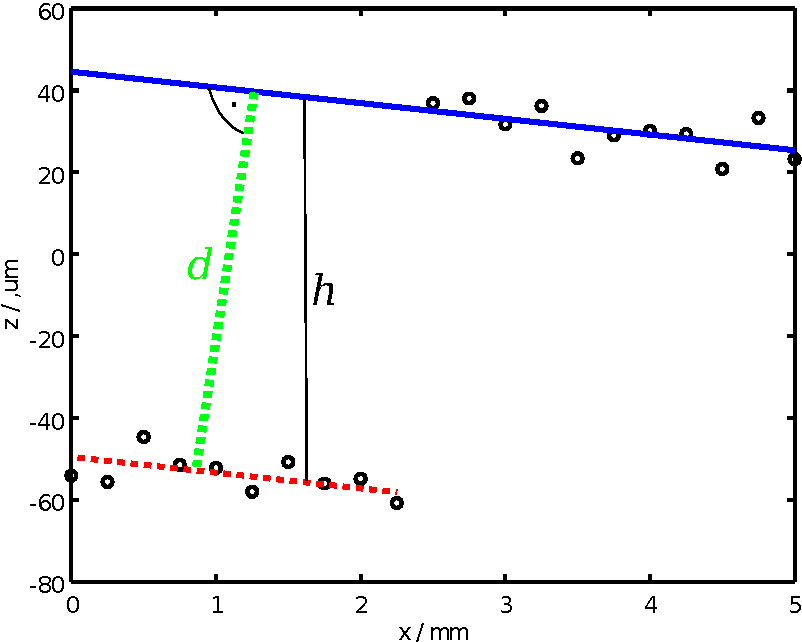
\includegraphics[width=90mm]{03_vorlesung/media/uebungA5_step_plot.pdf}
\end{center}

%\vspace{2mm}

\begin{tabular}{l|c|c|c|c|c|c|c|c|c|c}
	\hline
	$x / \mathrm{mm}$ &
	0.00 & 0.25 & 0.50 & 0.75 & 1.00 & 1.25 & 1.50 & 1.75 & 2.00 & 2.25 \\
	\hline
	$z / \mathrm{\mu m}$ &
	-54.08 &-55.63 &-44.65 &-51.44 &-52.21 &-58.01 &-50.76 &-56.01 &-54.86 &-60.77\\ 
	\hline
\end{tabular}

\vspace{2mm}

\begin{tabular}{l|c|c|c|c|c|c|c|c|c|c|c}
	\hline
	$x / \mathrm{mm}$  & 2.50 &
	2.75 & 3.00 & 3.25 & 3.50 & 3.75 & 4.00 & 4.25 & 4.50 & 4.75 & 5.00 \\
	\hline
	$z / \mathrm{\mu m}$ &36.85 &38.02 &31.71 &36.21 &23.39 &29.01 &30.11 &29.35 &20.81 &33.27 &23.19\\
	\hline
\end{tabular}

\vspace{2mm}

Die Modellgleichung, mit der die Stufe beschrieben wird, ist
$$
z_j \; = \; a \, x_j \, + \, c \, + \, h \, \delta_{j \in C} \; + \; \varepsilon_j
$$
mit $C$ Menge der Indizes von 1 bis $J_C$. Hier sei $J_C = 10$:
$$
C \; = \; \{\, j \, | \, j = 1, 2, \dots, J_C \}
$$
und
$$
\delta_{j \in C} \; = \; \left\{
\begin{array}{ll}
1 & \mathrm{falls} \; \;  j \in C \; \mathrm{~d.h.~} j = 1 \; \mathrm{~oder} \; j = 2
\mathrm{~oder} \; \dots \; j = J_C\\
0 & \mathrm{sonst}
\end{array} \right.
$$
Dabei ist $h$ noch nicht die Stufenhöhe, sondern deren Projektion auf die vertikale Achse.
Die Stufenhöhe $d$ ist der senkrechte Abstand zwischen den beiden parallelen Geraden, die jeweils durch die Punkte auf dem oberen und dem unteren Niveau gehen.

\begin{itemize}
	\item[a)] Stellen Sie das lineare Gleichungssystem auf, das sich durch partielles Ableiten
	für das Optimierungsproblem
	$$
	\min\limits_{a,c,h} \left\{\sum_{j=1}^{J_T} \varepsilon_j^2\right\}
	$$
	ergibt, mit $J_T = 21$.
	\item[b)] Schreiben Sie die Gleichung für die Stufenhöhe $d$ als Funktion von $h$ und $a$ auf.
	\item[c)] Schreiben Sie die Gleichung für die Varianz der Residuen auf.
	\item[d)] Schreiben Sie die Formel für die Kovarianzmatrix der Modellparameter
	$a, c, h$ auf.
	\item[e)] Verwenden Sie eine Programmierumgebung Ihrer Wahl, Matlab, Octave, Python, R, ...
	die Ihnen einen Solver für lineare Gleichungssysteme zur Verfügung stellt, sowie
	eine Routine zur Matrixinversion und berechen Sie die Zahlenwerte für die Modellparameter
	sowie deren Kovarianzmatrix.
\end{itemize}
Anmerkung: Die inverse Matrix brauchen Sie nicht analytisch zu berechnen, sondern
	lediglich $(...)^{-1}$ zu notieren


\subsection{2. Aufg zur Linearen Regression}
\label{Vorl3Regressionsaufg2}

Gegeben sind 5 Messpunkte
\begin{table}[htb!]
	\centering
	\begin{tabular}{l|c c c c c c}
		$X_i$ & 1 & 2 & 3 & 4 & 5 \\ \hline
		$Y_i$ & 0.4 & 0.55 & 0.70 & 0.75 & 0.8
	\end{tabular}
\end{table}
\begin{itemize}
	\item [(a)] Führen Sie eine lineare Regression durch, indem
	Sie den y-Abschnitt $\hat\theta_0$ und die Steigung $\hat\theta_1$ bestimmen. Geben Sie das Bestimmtheitsmaß $\rho_{XY}^2$ an.
	\item[(b)] Bestimmen Sie die Residuen $\varepsilon_j$ und das 
	Qualitätsmaß $Q(\hat\theta _0,\hat\theta _1)$ der Regression. Geben Sie die Varianz der Residuen 
	$s^2(\hat\theta_0,\hat{\theta_1})$ an?
	\item[(c)] Geben Sie den Standardabweichung (standard error) der beiden 
	Regressionsparameter $\hat\theta_0$ und $\hat\theta_1$ an?
	
	% Geben Sie das 95\%ige Vertrauensintervall
	% von	$\hat\theta_0$ und $\hat\theta_1$ an.
% 	Es wird dazu das t-Quantil für 3 Freiheitsgrade (5 Messpunkte minus
%	2 Parameter = 3 Freiheitsgrade) benötigt.
%	Das t-Quantil für den beidseitigen Vertrauensbereich von 95\%
%	für 3 Freiheitsgrade ist gegeben durch $t_3=3.1824$. 
%		\newline
%	Man erhält das t-Quantil durch den Matlab/Octave-Befehl: \texttt{tinv(0.975,3) = 3.31824} (\texttt{tinv} berechnet den einseitigen Vertrauensbereich)
%	oder man schlägt in einem Tabellenwerk nach;
%	siehe z.~B. https://de.wikipedia.org/wiki/Studentsche\_t-Verteilung
\end{itemize}



%
\chapter{Optimierung nichtlinearer Modelle}
%
\chapter{Wahrscheinlichkeiten und Hypothesentests}
%
\chapter{Auswertung von Mess- und Ringvergleichen}
%
\chapter{Messunsicherheitsfortpflanzung\\ linearer Modelle}
%
\chapter{Lösungen zu den Aufgaben\\ zum Selbststudium}
\section{Lösungen zu den Aufgaben aus Vorl 2}
\subsection{Lösung zur 1. Aufgabe: Lineare Regression}
siehe \ref{Vorl2Regressionsaufg1}

zu (a) Stellen Sie das lineare Gleichungssystem auf, das sich durch partielles Ableiten
für das Optimierungsproblem
$$
\min\limits_{a,c,h} \left\{\sum_{j=1}^{J_T} \varepsilon_j^2\right\}
$$
ergibt, mit $J_T = 21$.

Die Modellgleichung lautet
\begin{equation}
z_j \; = \; a \, x_j \, + \, c \, + \, h \, \delta_{j \in C} \; + \; \varepsilon_j
\label{Modellgl1}
\end{equation}
In Vektorschreibweise mit $\boldsymbol x$ und $\boldsymbol z$ als Spaltenvektoren sieht 
dies mit allen in der oben aufgeführten Werten wie folgt aus
$$
\boldsymbol x = \left(
\begin{array}{c}
0\\
0.25\\
0.50\\
\vdots\\
2.25\\
2.75\\
\vdots\\
5.00
\end{array}\right) \qquad
\boldsymbol x_1 = \left(
\begin{array}{c}
1\\
1\\
1\\
\vdots\\
1\\
0\\
\vdots\\
0
\end{array}\right)  \qquad
\boldsymbol x_0 = \left(
\begin{array}{c}
1\\
1\\
1\\
\vdots\\
1\\
1\\
\vdots\\
1
\end{array}\right) \qquad
\boldsymbol z = \left(
\begin{array}{c}
-54.08\\
-55.63\\
-44.65\\
\vdots\\
-60.77\\
36.85\\
\vdots\\
23.19
\end{array}\right)
$$
Für die Realisierung der Kroneckersymbols $\delta_{j \in C}$ wurde
der Spaltenvektor $\boldsymbol x_1$ definiert, der als erste
$J_C = 10$ Vektorkomponenten Einsen enthält und als weitere Vektorkomponenten Nullen.
Der Vektor $\boldsymbol x_0$ besteht nur aus Einsen.

Als nächstes ist es wichtig, die Größen auf dieselbe Dimension zu bringen,
so dass wir eine Steigung berechnen wollen, also rechnen wir die x-Werte auch in Mikrometern
$$
\boldsymbol x_2 \, = \, 1000 \, \boldsymbol x
$$
Somit sieht die Modellgleichung (\ref{Modellgl1}) wie folgt aus
$$
\boldsymbol z \; = \;  c \,  \boldsymbol x_0 \,  + \, h \, \boldsymbol x_1 \, + \, a \, \boldsymbol x_2 \, + \, \boldsymbol \varepsilon
$$
nun schreiben wir alle Spaltenvektoren mit x in eine gemeinsame Matrix, die dann 3 Spalten hat und $J_T = 21$ Zeilen
\begin{equation}
\boldsymbol X \; = \; \left(\boldsymbol x_0 \; \boldsymbol x_1 \; \boldsymbol x_2 \right)
\label{Regressormatrix}
\end{equation}
so dass die Modellgleichung wie folgt aussieht
$$
\boldsymbol \varepsilon  \; = \;  \boldsymbol z \, - \, \boldsymbol X
\left(\begin{array}{c}
c\\
h\\
a
\end{array}\right) .
$$
Wenn man diesen Ansatz in dieser Form hat, kann man einfach Gl.~(\ref{LsgRegressionGlSys}) 
verwenden und alles einsetzten.
Für die Klausur kommt es also nur darauf an, die Regressormatrix $\boldsymbol X$, das ist Gl.~(\ref{Regressormatrix})
aufstellen zu können und Gl.~(\ref{LsgRegressionGlSys}) aus dieser Vorlesung zu kennen:
\begin{equation}
\left( \mathbf{X}^\mathsf{T}  \, \mathbf{X} \right) \left(\begin{array}{c}
c\\
h\\
a
\end{array}\right) \; = \;
 \mathbf{X}^\mathsf{T} \, \mathbf{z} 
\end{equation}
wobei $\boldsymbol X^\mathsf{T}$ die transponierte Matrix ist, die in der ersten Zeile alles Einsen hat, in der
zweiten Zeile an den ersten $J_C = 10$ Spaltenpositionen Einsen und an den letzten 11 Nullen hat und in der dritten
und letzten Zeile die Werte $0.00 ~ 0.25 ~ 0.50 ~ 0.75 \dots ~5.00$ aus der Tabelle hat.
Hier ist dieser Teil der Aufgabenstellung fertig.


zu (b) Schreiben Sie die Gleichung für die Stufenhöhe $d$ als Funktion von $h$ und $a$ auf.
\begin{equation}
d \; = \; \frac{h}{\sqrt{1 + a^2}}
\end{equation}
Wer zuvor die x-Werte in Millimetern gerechnet hat, muss spätestens hier die Steigung
$a$ entsprechend umrechnen und durch $1000$ teilen.

zu (c) Schreiben Sie die Formel für die Varianz der Residuen auf.
$$
\sigma_\varepsilon^2 \; = \; \frac{1}{J_T - 3} \boldsymbol \varepsilon^\mathsf{T} \, \boldsymbol \varepsilon
$$

zu (d) Schreiben Sie die Formel für die Kovarianzmatrix der Modellparameter
$a, c, h$ auf.

Wir verwenden dazu Gl.~(\ref{UnsicherheitRegressparams}) dieser Vorlesung
\begin{equation}
\boldsymbol \Sigma \; = \; \left( \mathbf{X}^\mathsf{T}  \, \mathbf{X} \right)^{-1} \, \sigma_\varepsilon^2
\end{equation}
mit 

zu (e) Verwenden Sie eine Programmierumgebung Ihrer Wahl, Matlab, Octave, Python, R, ...
die Ihnen einen Solver für lineare Gleichungssysteme zur Verfügung stellt, sowie
eine Routine zur Matrixinversion und berechen Sie die Zahlenwerte für die Modellparameter
sowie deren Kovarianzmatrix.

\begin{verbatim}
function Lsg_Uebung_step()
%
% Teil (a)
  x = [0.00  0.25  0.50  0.75  1.00  1.25  1.50 ...
   1.75  2.00  2.25  2.50  2.75  3.00  3.25  3.50 ...
   3.75  4.00  4.25  4.50  4.75  5.00]';
  z = [-54.08 -55.63 -44.65 -51.44 -52.21 -58.01 ...
   -50.76 -56.01 -54.86 -60.77 36.85 38.02 31.71 36.21 ...
   23.39 29.01 30.11 29.35 20.81 33.27 23.19]';
  x2 = 1e3*x;
  J_T = 21;
  J_C = 10;
  x0 = ones(J_T,1);
  x1 = [ones(J_C,1);zeros(J_T-J_C,1)];
  X = [x0 x1 x2];
  XTX = X' * X;
  b = X' * z;
  theta = XTX \ b;
  printf('c = %1.4f um\n', theta(1));
  printf('h = %1.4f um\n', theta(2));
  printf('a = %1.7f um/um\n', theta(3));
\end{verbatim}
\begin{verbatim}
%
% Teil (b)
  d = theta(2) / sqrt(1 + theta(3)^2);
  printf('d = %1.4f um\n', d);
\end{verbatim}
\begin{verbatim}
%
% Teil (c)
  epsilon = z - X * theta;
  var_eps = (epsilon' * epsilon) / (J_T-3);
\end{verbatim}

~\\

\begin{verbatim}
%
% Teil (e)
  Kovarianz = inv(XTX) * var_eps;
  printf(' %e %e %e \n', Kovarianz(1,1), Kovarianz(1,2), Kovarianz(1,3));
  printf(' %e %e %e \n', Kovarianz(2,1), Kovarianz(2,2), Kovarianz(2,3));
  printf(' %e %e %e \n', Kovarianz(3,1), Kovarianz(3,2), Kovarianz(3,3));
\end{verbatim}

Ergebnisse:
\begin{verbatim}
c = 44.5660 um
h = -94.0905 um
a = -0.0038377 um/um
d = -94.0899 um
\end{verbatim}

$\Sigma =$
\begin{verbatim}
2.369818e+01 -1.710178e+01 -5.863466e-03
 -1.710178e+01 1.436549e+01 4.104426e-03
 -5.863466e-03 4.104426e-03 1.563591e-06
\end{verbatim}



\subsection{Lösung zur 2. Aufgabe: Lineare Regression}
siehe \ref{Vorl2Regressionsaufg2}

\textbf{zu Teil (a)} \\
Gesucht: 
\[
Y = \hat\theta_1 \cdot X + \hat \theta_0 
\]
Mittelwert von $X$: $\bar{X} = 3$; Mittelwert von $Y$: $\bar{Y} = 0.64$; \\
Empirische Standardabeichung von $X$: $s_X = 1.5811$; \\
Empirische Standardabeichung von $Y$: $s_Y = 0.1636$; \\
Empirische Kovarianz: $s_{XY} = 0.25$ \\
Schätzwerte $\hat{\theta}_1$ und $\hat{\theta}_0$:
\[
\hat{\theta}_1 = \frac{s_{XY} }{s_X^2 } = 0.100
\]
\[
\hat{\theta}_0 = \bar {Y} - \hat{\theta}_1 \bar {X} = 0.340
\]
Bestimmtheitsmaß:
\[
\rho_{XY}^2 = \frac{s
_{XY}^2 }{s_X^2 \cdot s_Y^2 } = 0.9346
\]
\textbf{zu Teil (b)} \\
Residuen: $\varepsilon_j = Y_j -(\hat\theta _0 + \hat\theta _1 \cdot X_j)$
mit $j=1,\ldots ,5$
 \[\varepsilon_1 = -0.0400; \;\; \varepsilon_2 =  0.0100;\;\;
 \varepsilon_3= 0.0600;\;\; \varepsilon_4 =0.0100;\;\;
  \varepsilon_5 = -0.0400
 \]
Qualitätsmaß:
\[
Q(\hat\theta _0,\hat\theta _1) = \sum\limits_{j = 1}^J {\varepsilon_j ^2 } 
= 0.0070
\]
Varianz der Residuen:
\[
s^2(\hat{\theta}_0 ,\hat{\theta}_1 ) = \frac{Q(\hat{\theta}_0 ,
	\hat{\theta}_1 )}{J - 2} = 0.0023 \quad \text{bzw.} \quad
     s(\hat{\theta}_0 ,\hat{\theta}_1 ) = 0.048 
\]
\textbf{zu Teil (c)} \\
Die Standardabweichung für $X$ berechnet sich zu $s_X = 1.5811$.

Für die Varianz des y-Abschnitt $\hat\theta_0$ ergibt sich: 
\begin{eqnarray}
\hat\sigma_{\theta_0}^2 &=& s^2(\hat{\theta}_0 ,\hat{\theta}_1 )
\left[\frac{1}{J} + \frac{\bar{X}^2}{(J-1)s_x^2 } \right]
\nonumber \\ 
&=& 
0.0023
\left[\frac{1}{5} + \frac{3^2}{(5-1)\cdot 1.5811^2 } \right]
 \nonumber\\ 
&=& 0.00253 \nonumber
\end{eqnarray}
Damit ergibt sich die Standardabweichung für $\hat\theta_0$:
\[
s_{\hat\theta_0} = \sqrt{\hat\sigma_{\theta_0}^2} = 0.0503
\]
Für die Varianz der Steigung $\hat\theta_1$ ergibt sich: 

\begin{eqnarray}
\hat\sigma^2_{\theta_1} &=& \frac{ \hat s^2(\hat{\theta}_0 ,\hat{\theta}_1 )}
{s^2_X \cdot (J- 1) }
\nonumber \\
&=& \frac{ 0.0023}
{1.5811^2 \cdot (5- 1) } \nonumber \\
&=& 0.00023
\end{eqnarray}

Damit ergibt sich die Standardabweichung für $\hat\theta_1$
\[
s_{\hat\theta_1} = \sqrt{\hat\sigma_{\theta_1}^2} = 0.01517
\]

\newpage
\textbf{Anmerkung: Lösung mit Matlab/Octave} 
Bei Matlab gibt es den Befehl \glqq polyfit\grqq ~mit dem Polynomfits durchgeführt werden können. Matlab liefert hier dasselbe Ergebnis, auch für die Vertrauensbereiche, das Qualitätsmaß $Q$ (engl. SSE: Sum sqared error) oder das Bestimmheitsmaß $\rho^2_{XY}$ (R-square), siehe Abb.\ref{fig:MatlabPolyfit}:
\begin{figure}[!htp]
	\begin{center}
		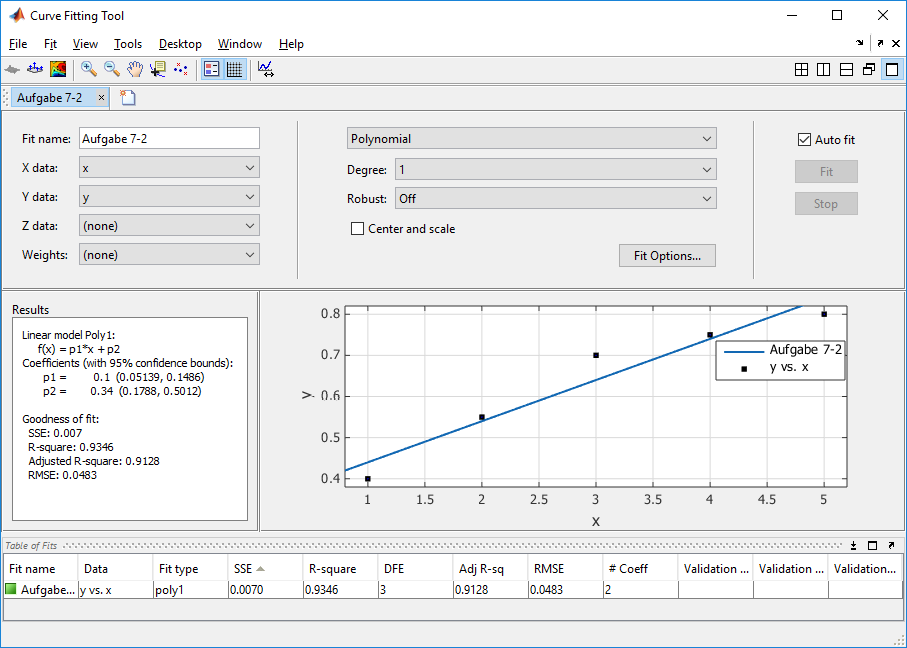
\includegraphics[width=160mm]{02_vorlesung/media/Matlab_CFTool.png}
		\caption{Lösung der Aufgabe mit dem polyfit Befehl von Matlab/Octave. 
		Es wird hier u.~a. der 95\%ige Vertrauensbereich berechnet und
		angezeigt (siehe Mitte links in der Abbildung).}
		\label{fig:MatlabPolyfit}
	\end{center}
\end{figure}

\textbf{Hinweis: Vertrauensbereich} \\
In einer der nächsten Vorlesungen werden wir sehen wie man Vertrauensbereiche 
mit Hilfe der Varianzen bzw. Standardabweichungen berechnet. Dazu benötigt man 
noch die t-Verteilung. Da man hier 5 Messpunkte und 2 Modellparameter hat,
wird die t-Verteilung mit dem Freiheitsgrad 5-2 = 3 benötigt. 
95\%iger Vertrauensbereich für $\hat\theta_1$ mit $t_3 = 3.182$: 
\[
\varepsilon _{\hat{\theta}_1} = t_3 \cdot \hat\sigma_{\theta_1} = \frac{t_3 \cdot s(\hat{\theta}_0 ,
	\hat{\theta}_1 )}{s_X \cdot \sqrt {J
		- 1} } = 0.0486
\]
95\%iger Vertrauensbereich für $\hat\theta_0$ errechnet sich durch:
\[
\varepsilon _{\hat{\theta}_0} = t_3 \cdot \hat\sigma_{\theta_0} = t_3 \cdot s(\hat{\theta}_0 ,\hat{\theta}_1 ) \cdot \sqrt {\frac{1}{J} + \frac{\bar {X}^2}{(J - 1) s_X^2 }} = 0.1612
\]
\textbf{Ergebnis:} \\ 
Der 95\% Vertrauensbereich des Schätzwertes $\hat\theta_1$ ist somit gegeben durch:
\begin{equation}
\hat\theta_1 = 0.1000 \pm 0.0486 \quad \text{bzw.} \quad [0.0514;0.1486]
\end{equation}
Der 95\% Vertrauensbereich des Schätzwertes $\hat\theta_0$ ist somit gegeben durch: 
\begin{equation}
\hat\theta_1 = 0.3400 \pm 0.1612 \quad \text{bzw.} \quad [0.1788;0.5012]
\end{equation}


\begin{comment}
95\%iger Vertrauensbereich für $\hat\theta_1$ mit $t_3 = 3.182$ und 
Standardabweichung von $s_X = 1.5811$
\[
\varepsilon _{\hat{\theta}_1} = \frac{t_3 \cdot s(\hat{\theta}_0 ,
\hat{\theta}_1 )}{s_X \cdot \sqrt {J
- 1} } = 0.0486
\]
95\%iger Vertrauensbereich für $\hat\theta_0$ errechnet sich durch:
\[
\varepsilon _{\hat{\theta}_0} = t_3 \cdot s(\hat{\theta}_0 ,\hat{\theta}_1 ) \cdot \sqrt {\frac{1}{J} + \frac{\bar {X}^2}{(J - 1) s_X^2 }} = 0.1612
\]
\textbf{Ergebnis:} \\ 
Der 95\% Vertrauensbereich des Schätzwertes $\hat\theta_1$ ist somit gegeben durch:
\begin{equation}
\hat\theta_1 = 0.1000 \pm 0.0486 \quad \text{bzw.} \quad [0.0514;0.1486]
\end{equation}
Der 95\% Vertrauensbereich des Schätzwertes $\hat\theta_0$ ist somit gegeben durch: 
\begin{equation}
\hat\theta_1 = 0.3400 \pm 0.1612 \quad \text{bzw.} \quad [0.1788;0.5012]
\end{equation}
\end{comment}


\pagebreak

Für die Unermüdlichen, die lieber in C programmieren, hier die Routine zum Lösen
des linearen Gleichungssystems, haben wir eine Routine zum Lösen von linearen
Gleichungssystemen aus den Numerical Recipes abgedruckt:

B. P. Flannery, W. H. Press, S. A. Teukolsky, W. T. Vetterling. \textsl{Numerical Recipes
in C}. Cambridge University Press, 2.~Auflage (1992-2002)

Wichtig, diese Routine überschreibt den Vektor mit der Inhomogenität des Gleichungssystems
mit der Lösung, also den gewünschten Modellparametern und 
die Matrix \texttt{a} mit den Summen aus den Regressoren mit deren Inversen
\texttt{a}$^{-1}$, die Sie dann für die Kovarianz der Modellparameter brauchen.

\begin{verbatim}
void gaussjordan(double **a, int n, double **b, int m)
/*
* Linear equation solution by Gauss-Jordan elimination, equation (2.1.1) in
* Numerical Recipes.
* a[0..n-1][0..n-1] is the input matrix. b[0..m-1][0..n-1] is input
* containing the m right-hand side vectors.
* For most applications we have m = 1
* On output, a is replaced by its matrix inverse,
* and b is replaced by the corresponding set of solution vectors.
*/
int *indxc,*indxr,*ipiv;
int i,icol,irow,j,k,l,ll;
double big,tmp,pivinv;

// The integer arrays ipiv, indxr, and indxc are
// used for bookkeeping on the pivoting.
indxc = (int*)calloc( n, sizeof(int));
indxr = (int*)calloc( n, sizeof(int));

ipiv = (int*)calloc( n, sizeof(int));

/*	for (j=1;j<=n;j++) ipiv[j]=0;*/
/*	for (j=1;j<=n;j++) ipiv[j]=0;*/
/* calloc initializes to zero:
Allocates a block of memory for an array of num elements,
each of them size bytes long, and initializes all its bits to zero.
*/

/*
* This is the main loop over the columns to be reduced.
*/
for (i=0; i<n; i++) {
big=0.0;

// This is the outer loop of the search for a pivot element.
for (j=0; j<n; j++)
if (ipiv[j] != 1)
for (k=0; k<n; k++) {
if (ipiv[k] == 0) {
if (fabs(a[k][j]) >= big) {
big=fabs(a[k][j]);
irow=j;
icol=k;
}
}
}
++(ipiv[icol]);

/*
* We now have the pivot element, so we interchange rows, if needed,
* to put the pivot element on the diagonal. The columns are not
* physically interchanged, only relabeled:
* indxc[i], the column of the ith pivot element,
*           is the ith column that is reduced, while
* indxr[i] is the row in which that pivot element was originally located.
*          If indxr[i] !=
* indxc[i] there is an implied column interchange.
* With this form of bookkeeping, the solution b-s will end up in the
* correct order, and the inverse matrix will be scrambled by columns.
*/

if (irow != icol) {
for (l=0; l<n; l++) SWAP(a[l][irow],a[l][icol])
for (l=0; l<m; l++) SWAP(b[l][irow],b[l][icol])
}

/*
* We are now ready to divide the pivot row by the
* pivot element, located at irow and icol.
*/

indxr[i]=irow;
indxc[i]=icol;
if (a[icol][icol] == 0.0) printf("gaussj: Singular Matrix\n");
pivinv=1.0/a[icol][icol];
a[icol][icol]=1.0;
for (l=0; l<n; l++) a[l][icol] *= pivinv;
for (l=0; l<m; l++) b[l][icol] *= pivinv;

/*
* Next, we reduce the rows
* except, if (ll != icol), for the pivot one, of course.
*/
for (ll=0; ll<n; ll++)
if (ll != icol) {
tmp=a[icol][ll];
a[icol][ll]=0.0;
for (l=0; l<n; l++) a[l][ll] -= a[l][icol]*tmp;
for (l=0; l<m; l++) b[l][ll] -= b[l][icol]*tmp;
}
}
/*
* This is the end of the main loop over columns of the reduction.
*/

/*
* It only remains to unscramble the solution in view of the column interchanges.
* We do this by interchanging pairs ofcolumns in the reverse order
* that the permutation was built up.
*/
for (l=n-1; l>=0;l--) {
if (indxr[l] != indxc[l])
for (k=0; k<n; k++) SWAP(a[indxr[l]][k],a[indxc[l]][k]);
}
// And we are done.
free(ipiv);
free(indxr);
free(indxc);
}
\end{verbatim}





\begin{thebibliography}{------}
    \bibitem[Fla02]{Fla02} B. P. Flannery, W. H. Press, S. A. Teukolsky, and W. T. Vetterling. Numerical Recipes in C. Cambridge University Press, 2. edition (1992-2002)
%    \bibitem[Els07]{Els07} C. Elster: Calculation of unceratinty
%	in the presence of prior knowledge, Metrologia 44, 111-116, (2007)
%    \bibitem[Cox06]{Cox06} M.G. Cox, B.R.L. Siebert:The use of
%    a Monte Carlo method for evaluating ..., Metrologie 43, S178-88,
%    (2006)
%    \bibitem[GUMS1]{GUMS1} 
%    JCGM 101:2008; Evaluation of measurement data — Supplement 1 to the 
%    “Guide to the expression of uncertainty in measurement” — 
%    Propagation of distributions using a Monte Carlo method (2008); \newline 
%    https://www.bipm.org/utils/common/documents/jcgm/JCGM\_101\_2008\_E.pdf
%    \bibitem[Wue08]{Wue08} Gerd Wübbeler, Michael Krystek and Clemens Elster: % % %    Evaluation of measurement uncertainty
%    and its numerical calculation by a Monte Carlo method
%    Meas. Sci. Technol. 19 (2008) 084009 (4pp)
%   doi:10.1088/0957-0233/19/8/084009
\end{thebibliography}

\end{document}


